\documentclass[	a4paper,		% DIN A4
		titlepage, 		% Titelseite statt Titelkopf
		fontsize=12pt		% Schriftgröße 12 Punkt
		]{scrartcl} 		% 'article' aus dem 'Koma'-Script
\usepackage{ngerman}			% deutsches Tastaturlayout
\usepackage[ngerman]{babel}		% Neue deutsche Rechtschreibung
\usepackage{babelbib}			% Literaturverzeichnis mehrsprachig
\usepackage{pst-all,			% psTricks einbinden
	    graphicx}  			% Grafikpaket
\usepackage{xcolor}			% Farben verwenden, z.B. \color{black}
\usepackage[utf8]{inputenc}		% Textdateityp / Kodierung
\usepackage{pstricks}			% FH-Logo zeichnen lassen
% \usepackage{picins}			% Grafiken mit Textumfluss
\usepackage{float}			% zum Positionieren von Grafiken
\usepackage{fancyhdr}			% Kopfzeilen formatieren
\usepackage{helvet}			% Schriftart Helvetica
\usepackage{setspace}			% anderthalbzeiligen Zeilenabstand und so
%\usepackage{tikz}			% Zeichnen mit pgf und TikZ
\usepackage[titles]{tocloft} 		% ändert Verzeichnisse
\usepackage{listings}			% Programmcode listings
\usepackage[paper=a4paper,		% Ausgabegröße
	    left=30mm, 			% linker Seitenrand
	    right=25mm, 		% rechter Seitenrand
	    top=25mm,  			% oberer Seitenrand
	    includehead, 		% Kopfzeile bei der Berechnung der Body-Größe mit einbeziehen
	    bottom=25mm, 		% oberer Seitenrand
	    includefoot			% Fußzeile bei der Berechnung der Body-Größe mit einbeziehen
	    ]{geometry} 		% Layout der Seiten anpassen

%-------Hyperref und Hypercap als letztes Paket einbinden!-------
\usepackage[colorlinks=true,		% farbige Links aktivieren
	    linkcolor=black,		% Linkfarbe festlegen
	    %breaklinks=true,		% Links dürfen umgebrochen werden (Wichtig im Inhaltsverzeichnis)
 	    linktocpage=true,		% Abbildungsverzeichnis mit Bildern verlinken und Links nur auf die Zahlen setzen
 	    linkcolor=black,		% Dokument-interne Links
 	    citecolor=black, 		% Links zum Literaturverzeichnis
 	    urlcolor=blue,		% Farbe des verlinkten Textes, externe URLs
 	    filecolor=blue,		% Links auf lokale Dateien
%  	    frenchlinks=true,		% Links werden als smallcaps, anstatt farbig dargestellt.
	    pdfborder={0 0 0},		% Rahmen um Links auf 0 festlegen
	    ]{hyperref}			% anklickbare Links im Inhaltsverzeichnis
\usepackage[all]{hypcap}		% Erlaubt Links auf Abbildungen nicht nur unterhalb der caption zu setzen

\renewcommand{\familydefault}{\sfdefault}% Schriftart benutzen
% \columnsep 1cm			% 1 cm Abstand zwischen den Spalten
\setlength{\headheight}{34pt}		% Größe der Kopfzeile festlegen
\setlength{\topmargin}{1pt}

\DeclareGraphicsExtensions{.png,.jpg,.jpeg}

% COLORS (Tango)
\definecolor{LightButter}{rgb}{0.98,0.91,0.31}
\definecolor{LightOrange}{rgb}{0.98,0.68,0.24}
\definecolor{LightChocolate}{rgb}{0.91,0.72,0.43}
\definecolor{LightChameleon}{rgb}{0.54,0.88,0.20}
\definecolor{LightSkyBlue}{rgb}{0.45,0.62,0.81}
\definecolor{LightPlum}{rgb}{0.68,0.50,0.66}
\definecolor{LightScarletRed}{rgb}{0.93,0.16,0.16}
\definecolor{Butter}{rgb}{0.93,0.86,0.25}
\definecolor{Orange}{rgb}{0.96,0.47,0.00}
\definecolor{Chocolate}{rgb}{0.75,0.49,0.07}
\definecolor{Chameleon}{rgb}{0.45,0.82,0.09}
\definecolor{SkyBlue}{rgb}{0.20,0.39,0.64}
\definecolor{Plum}{rgb}{0.46,0.31,0.48}
\definecolor{ScarletRed}{rgb}{0.80,0.00,0.00}
\definecolor{DarkButter}{rgb}{0.77,0.62,0.00}
\definecolor{DarkOrange}{rgb}{0.80,0.36,0.00}
\definecolor{DarkChocolate}{rgb}{0.56,0.35,0.01}
\definecolor{DarkChameleon}{rgb}{0.30,0.60,0.02}
\definecolor{DarkSkyBlue}{rgb}{0.12,0.29,0.40}
\definecolor{blue}{rgb}{0.0, 0.0, 0.9}
\definecolor{DarkGreen}{rgb}{0.12,0.40,0.29}
\definecolor{DarkPlum}{rgb}{0.36,0.21,0.40}
\definecolor{DarkScarletRed}{rgb}{0.64,0.00,0.00}
\definecolor{Aluminium1}{rgb}{0.93,0.93,0.92}
\definecolor{Aluminium2}{rgb}{0.82,0.84,0.81}
\definecolor{Aluminium3}{rgb}{0.73,0.74,0.71}
\definecolor{Aluminium4}{rgb}{0.53,0.54,0.52}
\definecolor{Aluminium5}{rgb}{0.33,0.34,0.32}
\definecolor{Aluminium6}{rgb}{0.18,0.20,0.21}

\lstdefinelanguage{Qt}{
	% classes:
	morekeywords=[1]{class, public, private, protected, slots, signals, this},
	% variables:
	morekeywords=[2]{int, char, double, float, void, bool},
	% Qt Classes
	morekeywords=[3]{QAbstractButton, QFlag, QMutex, QStyleOptionTab, QAbstractEventDispatcher, QFlags, QMutexLocker, QStyleOptionTabBarBase, QAbstractExtensionFactory, QFocusEvent, QNetworkAccessManager, QStyleOptionTabV2, QAbstractExtensionManager, QFocusFrame, QNetworkAddressEntry,  QStyleOptionTabWidgetFrame, QAbstractFileEngine, QFont,
	QNetworkCookie, QStyleOptionTitleBar, QAbstractFileEngineHandler, QFontComboBox, QNetworkCookieJar,
	QStyleOptionToolBar, QAbstractFileEngineIterator, QFontDatabase, QNetworkInterface, QStyleOptionToolBox, QAbstractFontEngine, QFontDialog, QNetworkProxy, QStyleOptionToolBoxV2, QAbstractFormBuilder, QFontEngineInfo, QNetworkReply, QStyleOptionToolButton, QAbstractGraphicsShapeItem, QFontEnginePlugin, QNetworkRequest, QStyleOptionViewItem, QAbstractItemDelegate, QFontInfo, QStyleOptionViewItemV2, QAbstractItemModel, QFontMetrics, QObject, QStyleOptionViewItemV4, QAbstractItemView, QFontMetricsF, QObjectCleanupHandler, QStylePainter, QAbstractListModel, QFormBuilder, QStylePlugin, QAbstractMessageHandler, QFormLayout, QPageSetupDialog, QSvgGenerator, QAbstractPrintDialog, QFrame, QPaintDevice, QSvgRenderer, QAbstractProxyModel, QFSFileEngine, QPaintEngine, QSvgWidget, QAbstractScrollArea, QFtp, QPaintEngineState, QSyntaxHighlighter, QAbstractSlider, QFuture, QPainter, QSysInfo, QAbstractSocket, QFutureIterator, QPainterPath, QSystemLocale, QAbstractSpinBox, QFutureSynchronizer, QPainterPathStroker, QSystemSemaphore, QAbstractTableModel, QFutureWatcher, QPaintEvent, QSystemTrayIcon, QAbstractTextDocumentLayout, QGenericArgument, QPair, QTabBar, QAbstractUriResolver, QGenericReturnArgument, QPalette, QTabletEvent, QAbstractXmlNodeModel, QGLColormap, QTableView, QAbstractXmlReceiver, QGLContext, QPen, QTableWidget, QAccessible, QGLFormat, QPersistentModelIndex, QTableWidgetItem, QAccessibleBridge, QGLFramebufferObject, QPicture, QTableWidgetSelectionRange, QAccessibleBridgePlugin, QGLPixelBuffer, QPictureFormatPlugin, QTabWidget, QAccessibleEvent, QGLWidget, QPictureIO, QTcpServer, QAccessibleInterface, QGradient, QPixmap, QTcpSocket, QAccessibleObject, QGraphicsEllipseItem, QPixmapCache, QTemporaryFile, QGraphicsGridLayout, QPlainTextDocumentLayout, QTestEventList, QAccessibleWidget, QGraphicsItem, QPlainTextEdit, QTextBlock, QAction, QGraphicsItemAnimation,
	QPlastiqueStyle, QTextBlockFormat, QActionEvent, QGraphicsItemGroup, QPluginLoader, QTextBlockGroup, QActionGroup, QGraphicsLayout, QPoint, QTextBlockUserData, QApplication, QGraphicsLayoutItem, QPointer, QTextBoundaryFinder, QAssistantClient, QGraphicsLinearLayout, QPointF, QTextBrowser, QAtomicInt, QGraphicsLineItem, QPolygon, QTextCharFormat, QAtomicPointer, QGraphicsPathItem, QPolygonF, QTextCodec, QGraphicsPixmapItem, QPrintDialog, QTextCodecPlugin, QAuthenticator, QGraphicsPolygonItem, QPrintEngine, QTextCursor, QAxAggregated, QGraphicsProxyWidget, QPrinter, QTextDecoder, QAxBase, QGraphicsRectItem, QPrinterInfo, QTextDocument, QAxBindable, QGraphicsScene, QPrintPreviewDialog, QTextDocumentFragment, QAxFactory, QGraphicsSceneContextMenuEvent, QPrintPreviewWidget, QTextEdit, QAxObject, QGraphicsSceneDragDropEvent, QProcess, QTextEncoder, QAxScript, QGraphicsSceneEvent, QProgressBar,  QTextFormat, QAxScriptEngine, QGraphicsSceneHelpEvent, QProgressDialog, QTextFragment, QAxScriptManager, QGraphicsSceneHoverEvent, QProxyModel, QTextFrame, QAxWidget, QGraphicsSceneMouseEvent, QProxyScreen, QTextFrameFormat, QBasicTimer, QGraphicsSceneMoveEvent, QPushButton, QTextImageFormat, QBitArray, QGraphicsSceneResizeEven, QQueue, QTextInlineObject, QBitmap, QGraphicsSceneWheelEvent, QRadialGradient, QTextItem, QBoxLayout, QGraphicsSimpleTextItem, QRadioButton, QTextLayout, QBrush, QGraphicsSvgItem, QRasterPaintEngine, QTextLength, QBuffer, QGraphicsTextItem, QReadLocker, QTextLine, QButtonGroup, QGraphicsView, QReadWriteLock,
	QTextList, QByteArray, QGraphicsWidget, QHelpEvent, QAccessiblePlugin, QRect, QTextListFormat, QByteArrayMatcher, QGridLayout, QRectF, QTextObject, QCache, QGroupBox, QRegExp, QTextOption, QCalendarWidget, QHash, QRegExpValidator, QTextStream, QCDEStyle, QHashIterator, QRegion, QTextTable, QChar, QHBoxLayout, QResizeEvent, QTextTableCell, QCheckBox, QHeaderView, QResource,
	QTextTableCellFormat, QChildEvent, QHelpContentItem, QRubberBand, QTextTableFormat, QCleanlooksStyle, QHelpContentModel, QRunnable, QThread, QClipboard, QHelpContentWidget, QScreen, QThreadPool, QCloseEvent, QHelpEngine, QScreenCursor, QThreadStorage, QColor, QHelpEngineCore, QScreenDriverFactory, QTime, QColorDialog, QScreenDriverPlugin, QTimeEdit, QColormap, QHelpIndexModel, QScriptable, QTimeLine, QColumnView, QHelpIndexWidget, QScriptClass, QTimer, QComboBox, QHelpSearchEngine, QScriptClassPropertyIterator, QTimerEvent, QCommandLinkButton, QHelpSearchQuery, QScriptContext, QToolBar, QCommonStyle, QHelpSearchQueryWidget, QScriptContextInfo, QToolBox, QCompleter, QHelpSearchResultWidget, QScriptEngine, QToolButton, QConicalGradient, QHideEvent, QScriptEngineAgent, QToolTip, QContextMenuEvent,
	QScriptExtensionPlugin, QTransform, QCopChannel, QHostInfo, QScriptString, QTranslator, QCoreApplication, QHoverEvent, QScriptValue, QTreeView, QCryptographicHash, QHttp, QScriptValueIterator, QTreeWidget, QCursor, QHttpHeader, QScrollArea, QTreeWidgetItem, QCustomRasterPaintDevice, QHttpRequestHeader, QScrollBar, QTreeWidgetItemIterator, QDataStream, QHttpResponseHeader, QUdpSocket, QDataWidgetMapper, QIcon, QSemaphore, QUiLoader, QDate, QIconDragEvent, QSessionManager, QUndoCommand, QDateEdit, QIconEngine, QSet, QUndoGroup, QDateTime, QIconEnginePlugin, QSetIterator, QUndoStack, QDateTimeEdit, QIconEnginePluginV2, QSettings,
	QUndoView, QDBusAbstractAdaptor, QIconEngineV2, QSharedData, QDBusAbstractInterface, QImage, QSharedDataPointer, QUrl, QDBusArgument, QImageIOHandler, QSharedMemory, QUrlInfo, QDBusConnection, QImageIOPlugin, QShortcut, QUuid, QDBusConnectionInterface, QImageReader, QShortcutEvent,
	QValidator, QDBusContext, QImageWriter, QShowEvent, QVariant, QDBusError, QInputContext, QSignalMapper, QVarLengthArray, QDBusInterface, QInputContextFactory, QSignalSpy, QVBoxLayout, QDBusMessage, QInputContextPlugin, QSimpleXmlNodeModel, QVector, QDBusObjectPath, QInputDialog, QSize, QVectorIterator, QDBusReply, QInputEvent, QSizeF, QDBusServer, QInputMethodEvent, QSizeGrip, QDBusSignature, QIntValidator, QSizePolicy, QHostAddress, QDBusVariant, QIODevice, QSlider,  QWaitCondition, QDecoration, QItemDelegate, QSocketNotifier, QWebFrame, QDecorationDefault, QItemEditorCreator, QSortFilterProxyModel, QWebHistory, QDecorationFactory, QItemEditorCreatorBase, QSound, QWebHistoryInterface, QDecorationPlugin, QItemEditorFactory, QSourceLocation, QWebHistoryItem, QDesignerActionEditorInterface, QItemSelection, QSpacerItem, QWebHitTestResult, QDesignerContainerExtension, QItemSelectionModel, QSpinBox, QWebPage, QDesignerCustomWidgetCollectionInterface, QItemSelectionRange, QSplashScreen, QWebPluginFactory, QDesignerCustomWidgetInterface, QKbdDriverFactory, QSplitter, QWebSettings, QDesignerDynamicPropertySheetExtension, QKbdDriverPlugin, QSplitterHandle, QWebView, QDesignerFormEditorInterface, QKeyEvent, QSqlDatabase, QWhatsThis, QDesignerFormWindowCursorInterface, QKeySequence, QSqlDriver, QWhatsThisClickedEvent, QDesignerFormWindowInterface, QLabel, QSqlDriverCreator, QWheelEvent, QDesignerFormWindowManagerInterface, QLatin1Char, QSqlDriverCreatorBase, QWidget, QDesignerMemberSheetExtension, QLatin1String, QSqlDriverPlugin, QWidgetAction, QDesignerObjectInspectorInterface, QLayout, QSqlError, QWidgetItem, QDesignerPropertyEditorInterface, QLayoutItem, QSqlField, QWindowsMime, QDesignerPropertySheetExtension, QLCDNumber, QSqlIndex, QWindowsStyle, QDesignerTaskMenuExtension, QLibrary, QSqlQuery, QWindowStateChangeEvent, QDesignerWidgetBoxInterface, QLibraryInfo, QSqlQueryModel, QWindowsVistaStyle, QDesktopServices, QLine, QSqlRecord, QWindowsXPStyle, QDesktopWidget, QLinearGradient, QSqlRelation, QWizard, QDial, QLineEdit, QSqlRelationalDelegate, QWizardPage, QDialog, QLineF, QWorkspace, QDialogButtonBox, QLinkedList, QSqlResult, QWriteLocker, QDir, QLinkedListIterator, QSqlTableModel, QWSCalibratedMouseHandler, QDirectPainter, QList,
	QSslCertificate, QWSClient, QDirIterator, QListIterator, QSslCipher, QWSEmbedWidget, QDirModel, QListView, QSslConfiguration, QWSEvent, QDockWidget, QListWidget, QSslError, QWSGLWindowSurface, QDomAttr, QListWidgetItem, QSslKey, QWSInputMethod, QDomCDATASection, QLocale, QSslSocket, QWSKeyboardHandler, QDomCharacterData, QLocalServer, QStack, QWSMouseHandler, QDomComment, QLocalSocket, QStackedLayout, QWSPointerCalibrationData, QDomDocument, QMacPasteboardMime, QStackedWidget, QWSScreenSaver, QDomDocumentFragment, QMacStyle, QStandardItem, QWSServer, QDomDocumentType, QMainWindow, QStandardItemEditorCreator, QWSWindow, QDomElement, QMap,
	QStandardItemModel, QX11EmbedContainer, QDomEntity, QMapIterator, QStatusBar, QX11EmbedWidget, QDomEntityReference, QMatrix, QStatusTipEvent, QX11Info, QDomImplementation, QMdiArea, QString, QXmlAttributes, QDomNamedNodeMap, QMdiSubWindow, QStringList, QXmlContentHandler, QDomNode,
	QStringListModel, QXmlDeclHandler, QDomNodeList, QStringMatcher, QXmlDefaultHandler, QDomNotation,  QStringRef, QSqlRelationalTableModel, QXmlDTDHandler, QDomProcessingInstruction, QStyle, QXmlEntityResolver, QDomText, QMenu, QStyledItemDelegate, QXmlErrorHandler, QDoubleSpinBox,
	QMenuBar, QStyleFactory, QXmlFormatter, QDoubleValidator, QMessageBox, QStyleHintReturn, QXmlInputSource, QDrag, QMetaClassInfo, QStyleHintReturnMask, QXmlItem, QDragEnterEvent, QMetaEnum, QStyleHintReturnVariant, QXmlLexicalHandler, QDragLeaveEvent, QMetaMethod, QStyleOption, QXmlLocator, QDragMoveEvent, QStyleOptionButton, QXmlName, QDropEvent, QMetaProperty, QStyleOptionComboBox, QXmlNamePool, QDynamicPropertyChangeEvent, QMetaType, QStyleOptionComplex,
	QXmlNamespaceSupport, QMimeData, QStyleOptionDockWidget, QXmlNodeModelIndex, QMimeSource, QStyleOptionFocusRect, QMetaObject, QXmlParseException, QModelIndex, QStyleOptionFrame, QXmlQuery, QErrorMessage, QMotifStyle, QStyleOptionFrameV2, QXmlReader, QEvent, QMouseDriverFactory, QStyleOptionGraphicsItem, QXmlResultItems, QEventLoop, QMouseDriverPlugin, QStyleOptionGroupBox, QXmlSerializer, QMouseEvent, QStyleOptionHeader, QXmlSimpleReader, QExplicitlySharedDataPointer, QMoveEvent, QStyleOptionMenuItem, QXmlStreamAttribute, QExtensionFactory, QMovie,
	QStyleOptionProgressBar, QXmlStreamAttributes, QExtensionManager, QMultiHash, QStyleOptionProgressBarV2, QXmlStreamEntityDeclaration,QFile, QMultiMap,
	QStyleOptionQ3DockWindow, QXmlStreamEntityResolver, QFileDialog, QMutableHashIterator, QStyleOptionQ3ListView, QXmlStreamNamespaceDeclaration, QFileIconProvider,
	QMutableLinkedListIterator, QStyleOptionQ3ListViewItem, QXmlStreamNotationDeclaration, QFileInfo, QMutableListIterator, QStyleOptionRubberBand, QXmlStreamReader, QFileOpenEvent, QMutableMapIterator, QStyleOptionSizeGrip, QXmlStreamWriter, QFileSystemModel, QMutableSetIterator, QStyleOptionSlider, QFileSystemWatcher, QMutableVectorIterator, QStyleOptionSpinBox
	}, % KDE Classes
	morekeywords=[4]{KApplication, KXMLGuiWindow, KPushButton, KMenu, KTabBar, KTextEditor, KAboutData, ki18n, KGuiItem, KMessageBox, KCmdLineArgs, KActionCollection}, % Qt Macros
	morekeywords=[5]{Q_OBJECT, Q_PROPERTY, READ, WRITE, SLOT, SIGNAL, connect, disconnect},
	morekeywords=[6]{if, for, else, while, do, case, switch, foreach, forever, new},
	% pre compiler directives
	morecomment=[s]{/*}{*/},%
	morecomment=[l]//,% nonstandard
	morestring=[b]",%
	morestring=[b]',
	sensitive=true,
	moredelim=*[directive]\#,
	moredirectives={define,elif,else,endif,error,if,ifdef,ifndef,line,
	include,pragma,undef,warning, emit},
	basicstyle=\ttfamily\scriptsize,
  }[keywords,comments,strings,directives]%

\lstset{
  language=Qt,			% choose the language of the code
  showspaces=false,		% show spaces within strings adding particular underscores
  showtabs=false,		% show tabs within strings adding particular underscores
  frame=single,
  showstringspaces=false,	% underline spaces within strings
  keywordstyle=[1]{\color{DarkSkyBlue}},
  keywordstyle=[2]{\color{DarkScarletRed}},
  keywordstyle=[3]{\color{DarkGreen}},
  keywordstyle=[4]{\color{blue}},
  keywordstyle=[5]{\color{Chocolate}},
  keywordstyle=[6]{\bfseries},
  commentstyle={\color{Aluminium4}},
  stringstyle={\color{Chocolate}},
  tabsize=4,
  breaklines=true,
  breakatwhitespace=true,
  prebreak=\mbox{{\color{blue}\tiny$\searrow$}},
  postbreak=\mbox{{\color{blue}\tiny$\rightarrow$}},
  basicstyle={			% the size of the fonts that are used for the code
    %\ttfamily
    \scriptsize
    },
  xleftmargin=5pt,
  xrightmargin=5pt,
  rulecolor=\color{black!30},
  backgroundcolor=\color{white},% choose the background color. You must add \usepackage{color}
  captionpos=b,
  framesep=10pt,
  framexleftmargin=18pt,
  numbers=none,			% where to put the line-numbers
  numberstyle={\tiny},		% the size of the fonts that are used for the line-numbers
  stepnumber=1,			% the step between two line-numbers. If it's 1 each line will be numbered
  numbersep=15pt,		% how far the line-numbers are from the code
  escapeinside={\%*}{*)}%,      % if you want to add a comment within your code
%morecomment=[is]{///}{</summary>}
%morecomment=[l][keywordstyle]{//}
}
\lstloadlanguages{Qt,XML}


%-------SEITENLAYOUT FÜR PAKET fancyhdr-----------
\pagestyle{fancy}			% eigenen Seitenstil von fancyhdr aktivieren
\fancyhf{}%Löschung der Vorbelegung
%-------Kopfzeile-------
\fancyhead[L]{\resizebox*{1cm}{!}{%LaTeX with PSTricks extensions
%%Creator: inkscape 0.46
%%Please note this file requires PSTricks extensions
\psset{xunit=.5pt,yunit=.5pt,runit=.5pt}
\begin{pspicture}(800,600)
{
\newrgbcolor{curcolor}{0 0 0}
\pscustom[linestyle=none,fillstyle=solid,fillcolor=curcolor]
{
\newpath
\moveto(78.34211,462.87504)
\curveto(79.63005,350.25949)(80.91799,237.64387)(82.20581,125.02832)
\curveto(101.99252,125.02832)(121.77929,125.02832)(141.56606,125.02832)
\curveto(141.56606,170.84037)(141.56606,216.6526)(141.56606,262.46477)
\curveto(174.46576,262.46477)(207.36565,262.46477)(240.26553,262.46477)
\curveto(240.26553,281.04486)(240.26553,299.62506)(240.26553,318.2052)
\curveto(206.89726,318.2052)(173.52917,318.2052)(140.16108,318.2052)
\curveto(140.51231,349.26668)(140.86348,380.3281)(141.21471,411.38964)
\curveto(175.75376,411.38964)(210.29275,411.38964)(244.83163,411.38964)
\curveto(244.83163,429.54421)(244.83163,447.69896)(244.83163,465.85364)
\curveto(189.3352,464.86072)(133.83866,463.86797)(78.34211,462.87504)
\closepath
}
}
{
\newrgbcolor{curcolor}{0.94117647 0.64705884 0.07450981}
\pscustom[linestyle=none,fillstyle=solid,fillcolor=curcolor]
{
\newpath
\moveto(526.66082157,117.16311448)
\lineto(457.3157015,117.16311448)
\lineto(457.3157015,329.96798209)
\curveto(457.3155111,351.18394332)(455.14092763,366.61388808)(450.79194455,376.25786265)
\curveto(446.60367399,386.11562382)(439.27452229,391.04463395)(428.80446746,391.04490783)
\curveto(410.76331677,391.04463395)(391.27260564,378.29349905)(370.33227562,352.79146486)
\lineto(370.33227562,117.16311448)
\lineto(300.98715555,117.16311448)
\lineto(300.98715555,595.17042283)
\lineto(370.33227562,595.17042283)
\lineto(370.33227562,413.54693311)
\curveto(381.60779021,427.90505754)(394.73583117,439.79897329)(409.71643789,449.22871604)
\curveto(424.69675901,458.65779466)(438.95236178,463.37250001)(452.48328895,463.37284622)
\curveto(501.93474235,463.37250001)(526.66056183,423.1903522)(526.66082157,342.82628224)
\lineto(526.66082157,117.16311448)
}
}
{
\newrgbcolor{curcolor}{0 0 0}
\pscustom[linestyle=none,fillstyle=solid,fillcolor=curcolor]
{
\newpath
\moveto(198.57924413,47.99697332)
\lineto(208.37494229,36.74149818)
\curveto(215.31720799,28.95758824)(219.3240208,24.70703803)(220.39539273,23.98983482)
\curveto(221.43992962,23.3026367)(222.79517023,22.81161963)(224.46111863,22.51678211)
\curveto(226.13027742,22.27875677)(228.29412656,23.21039495)(230.95267256,25.31169943)
\curveto(232.35866516,26.45775251)(233.32971575,26.73025619)(233.86582723,26.12921129)
\curveto(234.45548912,25.46800652)(234.26947751,24.70855127)(233.30779185,23.85084327)
\curveto(232.94712071,23.52916964)(231.93342314,22.75997352)(230.26669609,21.5432526)
\curveto(226.87305887,19.05613714)(223.97411038,16.74042519)(221.56984193,14.59610979)
\curveto(219.52618297,12.77341425)(216.79333773,10.12020991)(213.371298,6.6364888)
\lineto(210.96741483,4.24969863)
\curveto(210.00569476,3.39196204)(209.25679647,3.26363163)(208.72071769,3.86470701)
\curveto(208.18463135,4.46577417)(208.62284881,5.39620682)(210.0353714,6.65600772)
\curveto(211.95879437,8.37146502)(212.85878399,10.14541905)(212.73534296,11.97787514)
\curveto(212.61188634,13.81030679)(210.70027277,17.04268216)(207.00049654,21.67501094)
\curveto(203.30396561,26.36415359)(198.2124017,32.34521706)(191.72578952,39.6182193)
\curveto(185.61446156,46.47039193)(180.68290634,51.75779008)(176.93110907,55.4804296)
\curveto(173.15256368,59.23301125)(170.48839063,61.52439703)(168.93858193,62.35459381)
\curveto(167.41889879,63.21146953)(165.99542746,63.50673412)(164.66816368,63.24038847)
\curveto(163.3141763,63.00396943)(161.35298283,61.87535837)(158.78457739,59.85455192)
\curveto(157.76930125,59.05686686)(157.02040296,58.92853645)(156.53788026,59.4695603)
\curveto(156.10906261,59.95035761)(156.28857535,60.59609747)(157.07641901,61.40678183)
\curveto(164.0537752,68.70882344)(177.98604271,81.67430953)(198.87326332,100.30327899)
\curveto(202.44964345,103.49286968)(204.44170656,105.1616288)(204.84945862,105.30956138)
\curveto(205.26046029,105.51414054)(205.66008884,105.51982334)(206.04834549,105.32660978)
\curveto(206.43984935,105.19004278)(208.69505728,103.47820262)(212.81397607,100.19108417)
\curveto(216.96293265,96.93056898)(219.11782727,95.21020091)(219.27866638,95.0299748)
\curveto(219.84153873,94.3987547)(219.8525,93.84195513)(219.31155023,93.35957442)
\curveto(218.92083953,93.01102716)(218.2771287,92.9765112)(217.38041583,93.25602643)
\curveto(206.57583957,96.83967397)(196.41006784,94.3830902)(186.88307014,85.88626777)
\curveto(183.60724976,82.9645317)(181.08153003,80.44209856)(179.30590336,78.31896078)
\curveto(177.53357738,76.25252358)(176.66973587,74.86154661)(176.71437624,74.1460257)
\curveto(176.73226893,73.46040958)(178.1821252,71.38103089)(181.0639494,67.90788341)
\curveto(183.97587491,64.46140376)(189.17100158,58.54572589)(196.64934499,50.16083206)
\curveto(199.13080131,52.15809351)(200.82232878,53.55881135)(201.72393247,54.3629898)
\curveto(206.05164884,58.22272962)(208.23947929,61.8197761)(208.2874304,65.15414004)
\curveto(208.33862424,68.54523088)(207.52476696,71.27278278)(205.84585611,73.33680394)
\curveto(204.7265807,74.71269542)(204.48250587,75.68212129)(205.11363088,76.24508446)
\curveto(205.7748091,76.83469879)(206.50746022,76.67874074)(207.31158643,75.77720985)
\curveto(207.57962534,75.4765982)(207.88462337,75.07412453)(208.22658146,74.56978763)
\curveto(209.57084264,72.63897723)(213.44606817,68.0822086)(219.85226966,60.89946804)
\lineto(224.51619259,55.67014275)
\curveto(225.64194638,54.40783717)(225.82916353,53.44166074)(225.07784458,52.77161055)
\curveto(224.4466996,52.20867085)(223.70064642,52.37965568)(222.83968279,53.28456555)
\curveto(220.33713268,55.90892036)(217.51050272,57.35393964)(214.35978442,57.61962771)
\curveto(211.18224314,57.91525363)(207.20421891,55.93216735)(202.42569979,51.67036291)
\curveto(201.64430965,50.97340368)(200.36215904,49.7489417)(198.57924413,47.99697332)
}
}
{
\newrgbcolor{curcolor}{0 0 0}
\pscustom[linestyle=none,fillstyle=solid,fillcolor=curcolor]
{
\newpath
\moveto(315.80856681,98.24090742)
\curveto(314.38949728,96.867351)(313.57480163,96.08678186)(313.36447741,95.89919764)
\curveto(312.25244484,94.90740023)(310.18524782,93.17163078)(307.16288017,90.69188409)
\curveto(304.16722759,88.18200491)(298.07122834,82.82605347)(288.87486413,74.62401372)
\lineto(277.42444496,64.41163076)
\curveto(277.00368028,64.03635978)(275.5245568,62.60924213)(272.98707006,60.13027352)
\curveto(270.47636676,57.62123354)(268.93551143,56.11207878)(268.36449945,55.60280473)
\curveto(266.08042289,53.56568663)(264.6703462,52.8476654)(264.13426513,53.4487389)
\curveto(263.70539759,53.92959369)(263.92836596,54.5871109)(264.8031709,55.4212925)
\curveto(267.55753963,58.20161009)(269.03667055,60.62698678)(269.24056809,62.69742984)
\curveto(269.4176483,64.79790352)(268.83203043,67.02754259)(267.48371272,69.38635374)
\curveto(266.10858119,71.77518213)(261.4942131,77.37245246)(253.64059462,86.17818154)
\lineto(239.29184391,102.35716755)
\curveto(234.62794899,107.58643647)(231.13081894,111.02351142)(228.80044326,112.66840271)
\curveto(226.50018881,114.33997523)(224.13125806,115.06005522)(221.69364389,114.82864485)
\curveto(219.25936105,114.65396495)(217.05855515,113.82426481)(215.09121959,112.33954194)
\curveto(214.04914072,111.57190942)(213.28684036,111.45860579)(212.80431622,111.99963071)
\curveto(212.32189175,112.54053408)(212.51643127,113.19967601)(213.38793536,113.97705847)
\curveto(213.59835956,114.16462462)(214.00245795,114.4980515)(214.60023175,114.97734012)
\curveto(219.62003354,118.96865064)(225.33061494,123.8189774)(231.73199308,129.52833495)
\lineto(239.5455231,136.73987298)
\curveto(240.3569924,137.46349892)(241.03075679,137.52481901)(241.56681828,136.92383344)
\curveto(242.04931365,136.38278359)(241.85477413,135.72364167)(240.98319914,134.94640568)
\curveto(238.84941778,133.04322887)(237.43648854,131.02763337)(236.74440717,128.89961312)
\curveto(236.08243116,126.79824166)(236.00687807,124.97717081)(236.51774766,123.43639512)
\curveto(237.03191894,121.9523327)(238.7096103,119.61749873)(241.55082677,116.4318862)
\lineto(260.20773144,94.78721167)
\lineto(270.9123375,82.96640106)
\curveto(274.20923697,79.269781)(276.50383502,76.99951655)(277.79613855,76.15560091)
\curveto(279.11846532,75.33843954)(280.67758201,74.92133597)(282.47349328,74.90428897)
\curveto(284.24256075,74.91724817)(286.43443442,76.08971917)(289.04912086,78.4217055)
\curveto(289.2594694,78.6093072)(291.86885095,81.09843734)(296.87727336,85.88910339)
\curveto(300.48529889,90.13225197)(302.38601064,95.44274846)(302.5794143,101.82060881)
\curveto(302.77273807,108.19836797)(302.19079625,113.2371843)(300.83358709,116.9370729)
\curveto(300.46723077,118.01324525)(300.52450021,118.7657973)(301.0053956,119.19473132)
\curveto(301.51626781,119.65033352)(302.09337264,119.51752585)(302.73671181,118.7963079)
\curveto(303.48718729,117.95474054)(305.74522548,114.54569755)(309.51083314,108.56916869)
\curveto(313.24954293,102.6225787)(315.34878539,99.17982838)(315.80856681,98.24090742)
}
}
{
\newrgbcolor{curcolor}{0 0 0}
\pscustom[linestyle=none,fillstyle=solid,fillcolor=curcolor]
{
\newpath
\moveto(318.7736937,206.26862441)
\curveto(322.64731004,203.67984061)(327.71208469,199.72534878)(333.96803284,194.40513704)
\curveto(334.03218352,194.03059537)(333.97410543,193.76295842)(333.7937984,193.60222537)
\curveto(333.58340911,193.41450475)(333.25079087,193.33368805)(332.79594269,193.35977501)
\curveto(327.74697525,194.84614426)(323.49849124,195.61659794)(320.05047793,195.67113835)
\curveto(316.60246339,195.72549119)(313.59509286,195.25562517)(311.02835731,194.26153889)
\curveto(308.46488801,193.32412554)(304.85399799,190.77814513)(300.19567639,186.62359004)
\curveto(295.80787535,182.71010262)(292.56452385,179.35877055)(290.46561215,176.56958378)
\curveto(290.49325389,176.05454044)(290.868916,175.391333)(291.59259961,174.57995948)
\curveto(291.78025636,174.36951184)(292.08525439,173.96703817)(292.50759463,173.37253726)
\curveto(294.35141617,170.7001394)(300.01764411,164.04449547)(309.50629547,153.40558549)
\curveto(309.90836733,152.95473051)(310.50130758,152.35040981)(311.285118,151.59262156)
\curveto(313.64960937,153.53952488)(315.25260087,154.88825919)(316.0940973,155.63882853)
\curveto(319.88084966,159.01609489)(322.11984758,162.01126146)(322.81109777,164.62433722)
\curveto(323.50559066,167.29414519)(322.8221077,171.05528817)(320.76064682,175.90777745)
\curveto(320.40813376,176.72645715)(320.42722605,177.31006085)(320.81792376,177.65859029)
\curveto(321.38894008,178.16779295)(322.06310879,177.98665549)(322.84043191,177.11517738)
\lineto(324.26835963,175.15113683)
\curveto(326.1454524,172.56239902)(328.20977457,170.00581708)(330.46133234,167.48138333)
\curveto(334.10668272,163.39403309)(337.4653223,159.77948188)(340.53726116,156.63771884)
\curveto(341.44858042,155.61584293)(341.61874174,154.85029313)(341.04774564,154.34106716)
\curveto(340.62697414,153.96575691)(340.01981575,154.07176045)(339.22626865,154.65907812)
\curveto(335.43223693,157.64245915)(331.83152926,159.01763043)(328.42413483,158.78459606)
\curveto(325.01672243,158.55144789)(319.94702161,155.43283993)(313.21501714,149.42876282)
\curveto(315.08156402,147.15439275)(318.19937077,143.56786605)(322.56844675,138.66917198)
\curveto(328.22411462,132.32783328)(332.04126949,128.50168672)(334.01992282,127.19072082)
\curveto(335.99854699,125.87970431)(338.3000631,125.47721578)(340.92447806,125.98325401)
\curveto(343.52204592,126.5192976)(346.86448291,128.61001215)(350.95179907,132.25540392)
\curveto(362.64260378,142.68217932)(366.59429509,153.43719296)(362.80688485,164.52047709)
\curveto(362.34305515,165.88743984)(362.33656371,166.77198349)(362.78741052,167.1741107)
\curveto(363.26822419,167.60291146)(363.8034981,167.48675528)(364.39323387,166.82564183)
\curveto(364.71483845,166.46493412)(364.98815821,166.00722748)(365.21319395,165.45252051)
\curveto(365.54210523,164.72061447)(367.00942164,162.1981516)(369.61514759,157.88512434)
\curveto(370.16173693,156.96965505)(371.6814412,154.11619866)(374.17426497,149.32474661)
\lineto(355.24537515,132.52341574)
\curveto(352.54051862,130.11101359)(348.45120493,126.67968089)(342.97742182,122.22940735)
\curveto(337.56044933,117.77584369)(332.80995725,113.75482018)(328.72593133,110.16632475)
\curveto(324.69874452,106.57456332)(322.52798475,104.77340828)(322.2136455,104.76285421)
\curveto(321.89930071,104.75229438)(321.66171731,104.83717659)(321.50089461,105.01750111)
\curveto(320.96480999,105.61856925)(321.19265251,106.36137299)(322.18442285,107.24591458)
\curveto(325.52036566,110.22116742)(326.92355403,113.06444888)(326.39399216,115.7757675)
\curveto(325.86441638,118.48705834)(322.54396138,123.26881695)(316.4326172,130.12105768)
\lineto(308.14525923,139.32233149)
\lineto(300.56090383,148.09838514)
\curveto(299.00628329,149.84144562)(295.96604381,153.03849638)(291.44017626,157.68954702)
\curveto(286.91761415,162.39734375)(284.25791094,165.01647361)(283.46105863,165.54694447)
\curveto(282.69433185,166.10409213)(281.62540874,166.36483332)(280.25428608,166.32916884)
\curveto(278.88649124,166.35023316)(276.58699674,165.54043396)(273.35579568,163.8997688)
\curveto(272.38682021,163.41317441)(271.70127848,163.39530994)(271.29916842,163.84617536)
\curveto(270.81674226,164.38707754)(271.10144247,165.12663185)(272.15326991,166.06484051)
\lineto(281.79193811,173.77102757)
\curveto(285.17178126,176.51553368)(293.21801271,183.55689574)(305.93065659,194.89513487)
\curveto(314.28556077,202.34658943)(318.56656886,206.13774882)(318.7736937,206.26862441)
}
}
{
\newrgbcolor{curcolor}{0 0 0}
\pscustom[linestyle=none,fillstyle=solid,fillcolor=curcolor]
{
\newpath
\moveto(344.22340309,229.37137101)
\curveto(348.19778707,228.54520659)(354.68727574,227.56111367)(363.69188857,226.41908929)
\lineto(393.03412562,222.56025872)
\lineto(421.23230451,218.89515923)
\curveto(416.68125178,224.60283254)(410.53254953,231.79944061)(402.78617932,240.48500505)
\curveto(396.96966079,247.00654378)(392.9478212,251.24369192)(390.72064849,253.19646218)
\curveto(388.46665025,255.17909146)(385.79799994,256.14447412)(382.71468954,256.09261305)
\curveto(379.66142734,256.06735576)(376.84249434,254.9021997)(374.25788211,252.59714137)
\curveto(373.05574533,251.52487958)(372.22683897,251.24425231)(371.77116054,251.75525873)
\curveto(371.50312752,252.05569853)(371.43571288,252.37328998)(371.56891642,252.70803405)
\curveto(371.70538631,253.09944223)(373.61338327,255.0439619)(377.29291303,258.5415989)
\curveto(380.94564414,262.06908422)(384.06431156,264.98545569)(386.64892465,267.29072206)
\lineto(392.77498359,272.67348301)
\lineto(393.76675217,273.55802011)
\curveto(394.69839891,274.38883044)(395.40546629,274.53381235)(395.88795646,273.99296628)
\curveto(396.31680664,273.51199119)(396.16572275,272.86462661)(395.43470432,272.0508706)
\curveto(392.6941244,269.01294835)(391.21052366,266.25982757)(390.98389762,263.79150001)
\curveto(390.76049912,261.37981441)(391.5589253,258.88131799)(393.37917855,256.29600325)
\curveto(395.22945867,253.73729189)(402.14532801,245.74101495)(414.1268073,232.30714842)
\lineto(434.90489395,208.10263995)
\curveto(435.97700419,206.90044523)(436.21255112,206.03133268)(435.61153543,205.49529969)
\curveto(435.46121203,205.36122948)(435.19722883,205.23370771)(434.81958504,205.112734)
\curveto(434.4450811,205.04851961)(431.75408906,205.37344087)(426.74660084,206.08749878)
\curveto(421.71221506,206.83150991)(415.59757987,207.63731049)(408.4026769,208.50490293)
\curveto(401.23777076,209.39919433)(395.50773733,210.19727564)(391.21255945,210.89914926)
\curveto(381.88302014,212.34497422)(376.06932489,213.17635853)(373.77145629,213.39330469)
\curveto(365.28586012,214.13489745)(360.06267177,214.81844731)(358.10187556,215.4439563)
\curveto(356.78686307,215.88983351)(355.91897091,215.92517298)(355.49819649,215.54997482)
\curveto(355.16763182,215.25506978)(355.52501772,214.52160259)(356.57035525,213.34957104)
\lineto(362.89248201,206.44252298)
\curveto(370.79971689,197.57667121)(377.35251753,190.71349001)(382.55090359,185.8529588)
\curveto(387.7492846,180.99236773)(391.01939564,178.32409201)(392.36124652,177.84812365)
\curveto(393.70632217,177.42896912)(395.44048176,177.32986133)(397.5637305,177.55079999)
\curveto(399.71699773,177.79849952)(401.52995242,178.57906123)(403.00260001,179.89248747)
\curveto(404.98611223,181.66153595)(406.29952936,182.18542941)(406.94285535,181.46416942)
\curveto(407.42530273,180.92317974)(407.11054896,180.1568213)(405.99859308,179.16509181)
\lineto(384.27471905,159.87097455)
\curveto(383.25289364,158.95963025)(382.51414797,158.75941536)(382.05847983,159.27032929)
\curveto(381.52239524,159.87139721)(381.75023776,160.61420096)(382.74200807,161.49874276)
\curveto(386.43859367,164.79564492)(388.17927443,167.80502963)(387.96405557,170.52690591)
\curveto(387.7220167,173.27880655)(385.22883591,177.31450454)(380.48450572,182.63401201)
\lineto(366.01147512,198.13557919)
\curveto(357.67540535,207.48219525)(352.51479464,212.75416229)(350.52962753,213.95149614)
\curveto(348.51771528,215.1787675)(345.55137444,216.17542411)(341.63059613,216.94146898)
\curveto(337.71314404,217.76424949)(334.47834274,217.30738122)(331.92618253,215.57086278)
\curveto(330.79719296,214.77967703)(330.04504522,214.59448893)(329.66973707,215.01529791)
\curveto(329.160509,215.58625653)(329.56704818,216.4614562)(330.88935584,217.64089955)
\lineto(344.22340309,229.37137101)
}
}
{
\newrgbcolor{curcolor}{0 0 0}
\pscustom[linestyle=none,fillstyle=solid,fillcolor=curcolor]
{
\newpath
\moveto(435.33449018,305.45126718)
\curveto(435.42223887,306.98633708)(435.21268743,308.31031116)(434.70583523,309.42319341)
\curveto(434.30297923,310.35882021)(434.32694568,311.02771044)(434.77773464,311.42986611)
\curveto(435.01817764,311.64420539)(435.42268035,311.73517472)(435.99124399,311.70277439)
\curveto(437.16658082,310.80838097)(439.41041573,308.89753889)(442.72275546,305.97024242)
\lineto(451.36345647,298.46007859)
\curveto(451.84592868,297.91903366)(451.75657663,297.35370618)(451.09540005,296.76409445)
\curveto(450.73475547,296.44236583)(450.15115177,296.46145812)(449.34458721,296.82137139)
\curveto(444.24040751,299.33769029)(438.95955282,300.50940468)(433.50200731,300.33651806)
\curveto(428.07129747,300.13341256)(423.5076405,298.38344727)(419.81102272,295.08661694)
\curveto(416.17457099,291.84324005)(414.40302059,288.29370728)(414.49636622,284.43800796)
\curveto(414.61983496,280.60897926)(415.78052118,277.46230218)(417.97842838,274.99796729)
\curveto(420.65887247,271.99255361)(423.71618264,270.59139428)(427.15036806,270.7944851)
\curveto(430.58459772,270.99746969)(436.34023717,272.89322553)(444.41730367,276.48175832)
\curveto(450.33215545,279.16696417)(455.03470721,280.85194817)(458.52497306,281.5367154)
\curveto(462.04527395,282.24815903)(465.67238886,282.08365078)(469.40632867,281.04319015)
\curveto(473.1402282,280.00260279)(476.25357999,278.08485008)(478.74639336,275.28992628)
\curveto(482.9814161,270.54140563)(484.80569179,264.533156)(484.21922591,257.26515938)
\curveto(483.63269012,249.99708359)(480.48435117,243.81667333)(474.77419959,238.72391007)
\curveto(469.63501472,234.14038314)(463.03178094,231.13793879)(454.96447845,229.71656799)
\curveto(454.69316718,227.96371582)(454.916525,226.38225741)(455.63455259,224.97218801)
\curveto(456.25184981,223.79603366)(456.29001953,222.96672298)(455.74906187,222.48425348)
\curveto(455.26819837,222.05538263)(454.37309777,222.36323321)(453.06375737,223.40780615)
\curveto(451.75440939,224.45236763)(446.11863189,229.89409911)(436.15640798,239.73301691)
\curveto(435.95498582,240.20085412)(436.10972347,240.66261885)(436.6206214,241.11831247)
\curveto(437.0714375,241.52035094)(437.72692567,241.51141128)(438.58708787,241.09149345)
\curveto(453.58854486,233.58857664)(465.23665979,233.53609959)(473.53146759,240.93406216)
\curveto(477.64878154,244.60620444)(479.76554359,248.70644223)(479.88176011,253.23478785)
\curveto(480.00116484,257.81992005)(478.62686166,261.72036958)(475.75884646,264.93614814)
\curveto(473.7753145,267.16006459)(471.32150897,268.64082022)(468.39742249,269.37841949)
\curveto(465.50335133,270.14271949)(462.51019893,270.17117063)(459.41795633,269.463773)
\curveto(456.355747,268.78307593)(451.9707867,267.16550656)(446.26306227,264.61106005)
\curveto(438.91783639,261.35149618)(433.48466255,259.60844152)(429.96352445,259.38189083)
\curveto(426.4456744,259.21211442)(423.29454235,259.72020218)(420.51011886,260.90615564)
\curveto(417.69894876,262.1220762)(415.43561723,263.69177213)(413.72011749,265.61524814)
\curveto(410.15520403,269.61232415)(408.79553074,274.76689233)(409.64109356,281.07896813)
\curveto(410.5167892,287.41772126)(413.58430402,292.93249072)(418.84364722,297.62329305)
\curveto(420.82721284,299.39228555)(423.18235207,300.92620796)(425.90907197,302.22506489)
\curveto(428.66589216,303.55055685)(431.80769509,304.62595654)(435.33449018,305.45126718)
}
}
{
\newrgbcolor{curcolor}{0 0 0}
\pscustom[linestyle=none,fillstyle=solid,fillcolor=curcolor]
{
\newpath
\moveto(505.14541248,324.73527346)
\curveto(512.04876985,328.24815253)(518.06229795,329.91525721)(523.18601482,329.7365925)
\curveto(528.33973372,329.58459369)(532.60526612,327.61525434)(535.98262481,323.82856854)
\curveto(539.60114351,319.77127425)(541.21017754,314.48836822)(540.80973171,307.97983463)
\curveto(540.43600322,301.44115274)(536.89818833,295.18317521)(530.19627644,289.20588327)
\curveto(528.93399399,288.08008131)(526.85339491,286.35933864)(523.95447296,284.04365012)
\curveto(522.10087379,282.55234383)(521.09895356,281.73969208)(520.94870928,281.60569243)
\curveto(511.69218816,273.35000004)(505.52145933,267.68458073)(502.43650425,264.60941753)
\curveto(501.35457094,263.64446493)(500.55896758,263.44749948)(500.04969178,264.01852059)
\curveto(499.78164787,264.31905282)(499.74428679,264.66344841)(499.93760844,265.05170837)
\curveto(500.1609786,265.4667636)(501.11863456,266.7525531)(502.81057918,268.90908073)
\curveto(503.82508743,270.1916125)(504.31610451,271.54685311)(504.28363188,272.97480662)
\curveto(504.25114552,274.40273543)(503.30285585,276.52475366)(501.43876001,279.3408677)
\curveto(499.57465613,282.15694429)(496.44466772,286.02938415)(492.04878536,290.95819892)
\curveto(487.706522,295.82684588)(484.26869043,299.80244418)(481.73528034,302.88500575)
\curveto(479.17509748,305.99753635)(477.18468882,308.35024222)(475.76404839,309.94313041)
\curveto(471.34138893,314.90191908)(467.59449381,318.70978942)(464.5233518,321.36675286)
\curveto(461.48232914,324.05039893)(459.25432965,325.48972798)(457.83934665,325.68474432)
\curveto(456.39763869,325.90968409)(454.4624407,325.23593457)(452.0337469,323.66349373)
\curveto(451.05502243,323.00632522)(450.33780241,322.93322779)(449.8820847,323.44420119)
\curveto(449.39965794,323.98510251)(449.59419746,324.64424444)(450.46570385,325.42162895)
\lineto(458.7909536,332.60392203)
\curveto(461.46575939,334.98941743)(463.92162369,337.28766924)(466.15855388,339.49868435)
\curveto(471.17672161,344.45980994)(474.45215571,347.62391743)(475.98486602,348.99101633)
\curveto(481.54479672,353.94969163)(487.04823774,356.67272911)(492.49520561,357.16013695)
\curveto(497.91212976,357.62054758)(502.49687833,355.74705171)(506.24946508,351.53964373)
\curveto(509.19791032,348.23366082)(510.6639989,344.44205252)(510.64773523,340.16480746)
\curveto(510.63144509,335.88740331)(508.79733934,330.74423045)(505.14541248,324.73527346)
\moveto(467.5694109,335.73875058)
\curveto(473.16906269,328.91570788)(477.79155437,323.46058178)(481.43689979,319.37335589)
\lineto(487.43250253,312.74166433)
\curveto(488.23663636,311.8400053)(488.86612904,311.37620411)(489.32098248,311.35025935)
\curveto(489.80590567,311.35101727)(490.61938092,311.86070002)(491.76141068,312.87930914)
\curveto(497.47159342,317.97204119)(501.13001945,323.09651864)(502.73669975,328.25275688)
\curveto(504.31656528,333.43891341)(502.90856222,338.4964177)(498.51268633,343.42528493)
\curveto(494.78691145,347.60264746)(490.72038097,349.56061379)(486.3130827,349.29918979)
\curveto(481.90905608,349.09444612)(477.79863592,347.2900565)(473.98180992,343.88601552)
\curveto(471.75786965,341.90242678)(469.62040545,339.18667452)(467.5694109,335.73875058)
\moveto(491.53232524,308.87083788)
\curveto(491.78168444,307.74419275)(492.73728906,306.24923384)(494.39914197,304.38595666)
\lineto(506.5475112,290.12959201)
\curveto(510.94337905,285.20077807)(513.51617101,282.55809352)(514.2658948,282.20153041)
\curveto(515.04563845,281.87172828)(516.34605784,282.16819097)(518.16715687,283.09091938)
\curveto(520.01826796,284.04040698)(522.55169954,285.94918286)(525.76745919,288.81725275)
\curveto(528.62251938,291.36361671)(530.58819011,293.81823089)(531.66447728,296.18110265)
\curveto(532.74394539,298.60076098)(532.98967467,301.6528001)(532.40166585,305.33722918)
\curveto(531.81358707,309.02156882)(530.05874019,312.50168021)(527.13711997,315.7775738)
\curveto(522.79482152,320.64619593)(518.16255924,322.93597186)(513.24031924,322.64690843)
\curveto(508.34810115,322.38452508)(503.09199183,319.74717846)(497.4719755,314.73486065)
\curveto(495.57860094,313.04614647)(493.5987195,311.09147417)(491.53232524,308.87083788)
}
}
{
\newrgbcolor{curcolor}{0 0 0}
\pscustom[linestyle=none,fillstyle=solid,fillcolor=curcolor]
{
\newpath
\moveto(504.74371052,373.10256229)
\lineto(527.32898612,393.24588459)
\curveto(528.62131462,394.39837867)(529.50870339,394.70418535)(529.99115509,394.16330554)
\curveto(530.47365199,393.62225706)(530.27423832,392.8778286)(529.39291347,391.93001791)
\curveto(527.44676255,389.81646779)(526.39163096,387.82320658)(526.22751553,385.95022831)
\curveto(526.06345283,384.07709781)(526.7964934,381.68216414)(528.42663945,378.76542013)
\curveto(530.08688741,375.87534237)(534.48194831,370.433214)(541.61183536,362.4390187)
\curveto(550.16236316,352.85187931)(556.35655751,346.45127892)(560.19443699,343.23719831)
\curveto(564.06235484,340.04985501)(568.43226606,338.65924521)(573.30418378,339.06536471)
\curveto(578.17930951,339.52828344)(583.14138207,342.01130417)(588.19041634,346.51443435)
\curveto(593.47980794,351.23192418)(596.60904717,355.8304717)(597.57814343,360.31009071)
\curveto(598.54714972,364.78960876)(597.66832602,369.37478395)(594.94166969,374.06563003)
\curveto(592.24498224,378.78315177)(584.98634947,387.76875552)(573.16574962,401.02246825)
\curveto(567.08119201,407.84453598)(562.39452026,411.67759317)(559.10572033,412.52165129)
\curveto(555.79010325,413.3955576)(552.74983404,412.59957222)(549.98490358,410.13369275)
\curveto(548.87292434,409.14183971)(548.03549007,408.96152576)(547.47259826,409.59275036)
\curveto(546.93652082,410.19372187)(547.40479185,411.15095864)(548.87741275,412.46446354)
\lineto(566.90956892,428.54695639)
\curveto(567.72100082,429.27054913)(568.39476521,429.33186922)(568.9308641,428.73091685)
\curveto(569.30610556,428.31004806)(569.20335145,427.75974736)(568.62260146,427.08001311)
\curveto(566.63336001,424.71219294)(565.59365952,422.48987624)(565.50349687,420.41305637)
\curveto(565.44336197,418.36281946)(566.54800658,415.73273575)(568.81743402,412.52279737)
\curveto(571.08682901,409.31265361)(574.74112264,404.8825981)(579.78032588,399.23261755)
\curveto(586.07926876,392.16994071)(591.15621021,385.93301763)(595.01116547,380.52182959)
\curveto(598.89608945,375.1373043)(601.05258649,370.45058796)(601.48066306,366.46166652)
\curveto(601.88183772,362.50268539)(600.99441922,358.20384256)(598.81840491,353.56512515)
\curveto(596.64554758,348.98317796)(593.00458912,344.41387535)(587.89551862,339.85720363)
\curveto(582.66616326,335.19325534)(577.46609555,332.03931534)(572.29529989,330.39537416)
\curveto(567.12771427,328.80824955)(562.66316509,328.79244385)(558.90163896,330.34795702)
\curveto(555.14334965,331.96028685)(550.8250325,335.50133631)(545.94667457,340.97111602)
\lineto(534.98986983,353.61920909)
\curveto(525.09916423,364.70893026)(518.57397636,371.0571428)(515.41428665,372.66386575)
\curveto(512.25792074,374.32732073)(509.09012976,373.79531854)(505.91090421,371.0678576)
\curveto(504.88912974,370.15645601)(504.15038407,369.95624113)(503.69466499,370.46721234)
\curveto(503.13182721,371.09827654)(503.4815087,371.97672565)(504.74371052,373.10256229)
}
}
{
\newrgbcolor{curcolor}{0 0 0}
\pscustom[linestyle=none,fillstyle=solid,fillcolor=curcolor]
{
\newpath
\moveto(633.26386207,436.00660709)
\curveto(639.01949099,437.90229931)(643.59329315,438.58212109)(646.98528228,438.04607446)
\curveto(650.35041878,437.53995008)(654.25977825,435.57670528)(658.7133724,432.15633416)
\curveto(664.55990062,427.65797331)(669.21571759,425.28128613)(672.68083727,425.0262655)
\curveto(676.11905295,424.80119316)(679.34939185,425.92857639)(682.37186366,428.40841856)
\curveto(683.2368585,429.07196687)(683.91062289,429.13328697)(684.39315884,428.59237902)
\curveto(684.87557149,428.05135868)(684.65097841,427.36541262)(683.71937892,426.5345388)
\curveto(675.30432014,419.02932883)(669.95397718,414.74310915)(667.66833399,413.6758669)
\curveto(665.38585039,412.66539978)(661.31607047,414.56650841)(655.45898205,419.37919852)
\curveto(649.79595596,424.09513508)(645.40128451,427.29828782)(642.27495452,428.98866636)
\curveto(639.15183489,430.73578939)(636.02385321,431.39942344)(632.8910001,430.97957051)
\curveto(629.76137613,430.6164581)(626.13790011,428.59884842)(622.02056118,424.92673543)
\curveto(620.4577766,423.53286824)(618.83203905,421.78613009)(617.14334366,419.68651574)
\curveto(618.6817415,417.6590733)(620.36227798,415.62355457)(622.18495812,413.57995343)
\curveto(629.07361956,405.85614641)(633.64169433,400.94604252)(635.88919615,398.84962704)
\curveto(638.10986754,396.78321221)(640.21521942,395.69315291)(642.20525808,395.57944585)
\curveto(644.19850726,395.5225501)(646.46916859,396.57643157)(649.0172489,398.74109341)
\curveto(650.12595504,399.67596211)(650.89475427,399.90298112)(651.3236489,399.42215113)
\curveto(651.83289875,398.8511064)(651.42635957,397.97590673)(650.10403013,396.7965495)
\lineto(627.78923687,376.8944646)
\curveto(626.49692859,375.7418826)(625.59613776,375.4511027)(625.08686167,376.02212404)
\curveto(624.63118915,376.53303099)(624.91426464,377.24415645)(625.936089,378.15550257)
\curveto(628.22015664,380.19261053)(629.48972125,381.94544322)(629.74478666,383.41400592)
\curveto(630.02989162,384.9093507)(629.78460382,386.60614921)(629.00892253,388.50440655)
\curveto(628.20642457,390.43268523)(626.1031166,393.30523391)(622.69899231,397.12206121)
\lineto(614.40676018,406.23804839)
\lineto(601.94770238,420.29825605)
\curveto(595.56834072,427.45095627)(591.18139597,432.03696983)(588.78685496,434.05631048)
\curveto(586.42243543,436.10233193)(584.48603191,437.15421409)(582.97763861,437.21196011)
\curveto(581.4425207,437.29963005)(579.00128629,436.25549689)(575.65392805,434.07955749)
\curveto(574.94243792,433.60676981)(574.39904042,433.58078175)(574.02373391,434.00159325)
\curveto(573.59491658,434.48238866)(574.01160839,435.28570385)(575.27381059,436.41154125)
\lineto(601.43872071,460.79967574)
\curveto(608.80186508,467.36659868)(615.39616663,470.7118139)(621.22164513,470.83533145)
\curveto(627.07718023,470.98545623)(631.82762772,469.01692552)(635.47300186,464.92973341)
\curveto(637.77814413,462.34503441)(639.20606299,459.38273679)(639.75676273,456.04283167)
\curveto(640.337482,452.72956338)(640.1400825,449.77458814)(639.16456365,447.17789708)
\curveto(638.18901194,444.58105646)(636.22211338,440.85729685)(633.26386207,436.00660709)
\moveto(615.13303206,421.94053526)
\curveto(620.79610736,427.20709253)(624.76196478,431.47261006)(627.03061623,434.73710065)
\curveto(629.2992591,438.00146655)(630.39501607,441.70370794)(630.31789043,445.84383592)
\curveto(630.2708032,450.01062113)(628.81324252,453.70191611)(625.94520404,456.91773194)
\curveto(622.91633437,460.31370009)(619.14911914,462.26882131)(614.64354703,462.78310144)
\curveto(610.13799111,463.2972008)(605.40579011,461.34295511)(600.44692982,456.92035853)
\curveto(597.7421314,454.50790249)(595.07345136,451.48024899)(592.4408817,447.83738897)
\curveto(599.45140442,439.250934)(605.14118706,432.50837882)(609.51024669,427.60970317)
\curveto(611.01129108,425.92664839)(612.885551,424.03692765)(615.13303206,421.94053526)
}
}
{
\newrgbcolor{curcolor}{0 0 0}
\pscustom[linestyle=none,fillstyle=solid,fillcolor=curcolor]
{
\newpath
\moveto(706.95581738,519.45662243)
\curveto(706.5650958,519.10807429)(705.73050664,519.22707558)(704.45204741,519.81362665)
\curveto(697.16288942,523.02523477)(690.17630399,524.29443222)(683.49227015,523.62122282)
\curveto(676.83828631,522.97462027)(671.22722445,520.61425458)(666.65906774,516.54011869)
\curveto(662.90238734,513.18951114)(660.28446301,508.80417625)(658.8052869,503.38410085)
\curveto(657.29935246,497.99392221)(657.55191804,491.93288783)(659.56298441,485.20097954)
\curveto(661.54729094,478.49900437)(664.92500052,472.47327974)(669.69612328,467.12378757)
\curveto(676.50438379,459.49014028)(684.67196071,454.9304968)(694.19887853,453.44484346)
\curveto(703.72577137,451.95913318)(711.91533028,454.27196286)(718.76757984,460.38333943)
\curveto(721.20188142,462.5544384)(722.94052571,464.77959277)(723.98351791,467.05880923)
\curveto(725.02642556,469.33794153)(725.6693426,471.85389067)(725.91227098,474.60666418)
\curveto(726.1851645,477.38614256)(726.16365371,479.25554319)(725.84773854,480.21487167)
\curveto(725.56178866,481.2008938)(724.10543352,483.1665571)(721.47866875,486.11186746)
\curveto(717.08275199,491.04059076)(713.52672778,493.69668481)(710.81058543,494.08015758)
\curveto(708.12443844,494.49029628)(705.33880845,493.40880205)(702.45368709,490.83567162)
\lineto(701.09640122,489.54419803)
\curveto(700.22482849,488.76681376)(699.5344126,488.66366276)(699.02515149,489.23474472)
\curveto(698.40863923,489.92591243)(698.58124877,490.70039445)(699.54298064,491.55819313)
\lineto(702.0126538,493.59896265)
\lineto(712.08020334,502.82081228)
\lineto(724.3262341,514.22842092)
\curveto(725.01742344,514.84482662)(725.64448276,514.83751167)(726.20741395,514.20647606)
\curveto(726.77025614,513.575262)(726.68780728,512.88119235)(725.96006714,512.12426504)
\curveto(724.25752671,510.28200059)(723.10167748,508.52266902)(722.49251597,506.84626506)
\curveto(721.88327289,505.16969737)(721.80528644,503.80511277)(722.25855638,502.75250718)
\curveto(722.7117452,501.69974604)(723.79609199,500.21169032)(725.51159998,498.28833556)
\curveto(731.78372212,491.25572838)(735.06275796,487.24642275)(735.34871735,486.26040666)
\curveto(735.63456945,485.27426802)(734.24680475,481.20367203)(731.1854191,474.04860649)
\curveto(728.12393449,466.89344282)(723.93347655,460.9437202)(718.6140327,456.19942077)
\curveto(709.80830167,448.34578006)(699.76029597,444.45638099)(688.46998546,444.53121188)
\curveto(677.17966142,444.60600366)(667.67470836,448.97112249)(659.95509776,457.62658144)
\curveto(654.64790217,463.57715438)(651.32258789,470.27014453)(649.97914492,477.70557196)
\curveto(648.63901484,485.19775164)(649.35913199,492.55797757)(652.13949854,499.78627185)
\curveto(654.89312008,507.04447008)(658.92965645,513.04577192)(664.24911975,517.79019538)
\curveto(669.23802875,522.23958781)(675.89081271,525.60998244)(684.20749157,527.90138939)
\curveto(686.55409296,528.53726316)(688.0579841,529.15009691)(688.71916951,529.73989249)
\curveto(689.65082297,530.5707157)(690.01025277,531.61973787)(689.79745998,532.88696217)
\curveto(689.6317604,533.98014815)(689.72923604,534.68761986)(690.08988719,535.00937942)
\curveto(690.78111076,535.62576433)(691.96415358,535.11606672)(693.63901919,533.48028504)
\curveto(696.25850428,530.90612703)(700.42005474,527.11734155)(706.12368305,522.11391723)
\curveto(706.45180703,521.86689272)(706.72309775,521.62321478)(706.937556,521.38288267)
\curveto(707.58082984,520.66150074)(707.58691696,520.01941464)(706.95581738,519.45662243)
}
}
\end{pspicture}
}} % Logo-skalieren und einfügen
\fancyhead[C]{}
\fancyhead[R]{Kaiser, Baß}
%-------Fußzeile:-------
\fancyfoot[L]{}
\fancyfoot[C]{\thepage}
\fancyfoot[R]{}
%--------------------------------------------------


\begin{document}			% Beginn des Textes
%---------TITELBLATT-----------------------------
\begin{titlepage}
\centering
\resizebox*{.25\textheight}{!}{%LaTeX with PSTricks extensions
%%Creator: inkscape 0.46
%%Please note this file requires PSTricks extensions
\psset{xunit=.5pt,yunit=.5pt,runit=.5pt}
\begin{pspicture}(800,600)
{
\newrgbcolor{curcolor}{0 0 0}
\pscustom[linestyle=none,fillstyle=solid,fillcolor=curcolor]
{
\newpath
\moveto(78.34211,462.87504)
\curveto(79.63005,350.25949)(80.91799,237.64387)(82.20581,125.02832)
\curveto(101.99252,125.02832)(121.77929,125.02832)(141.56606,125.02832)
\curveto(141.56606,170.84037)(141.56606,216.6526)(141.56606,262.46477)
\curveto(174.46576,262.46477)(207.36565,262.46477)(240.26553,262.46477)
\curveto(240.26553,281.04486)(240.26553,299.62506)(240.26553,318.2052)
\curveto(206.89726,318.2052)(173.52917,318.2052)(140.16108,318.2052)
\curveto(140.51231,349.26668)(140.86348,380.3281)(141.21471,411.38964)
\curveto(175.75376,411.38964)(210.29275,411.38964)(244.83163,411.38964)
\curveto(244.83163,429.54421)(244.83163,447.69896)(244.83163,465.85364)
\curveto(189.3352,464.86072)(133.83866,463.86797)(78.34211,462.87504)
\closepath
}
}
{
\newrgbcolor{curcolor}{0.94117647 0.64705884 0.07450981}
\pscustom[linestyle=none,fillstyle=solid,fillcolor=curcolor]
{
\newpath
\moveto(526.66082157,117.16311448)
\lineto(457.3157015,117.16311448)
\lineto(457.3157015,329.96798209)
\curveto(457.3155111,351.18394332)(455.14092763,366.61388808)(450.79194455,376.25786265)
\curveto(446.60367399,386.11562382)(439.27452229,391.04463395)(428.80446746,391.04490783)
\curveto(410.76331677,391.04463395)(391.27260564,378.29349905)(370.33227562,352.79146486)
\lineto(370.33227562,117.16311448)
\lineto(300.98715555,117.16311448)
\lineto(300.98715555,595.17042283)
\lineto(370.33227562,595.17042283)
\lineto(370.33227562,413.54693311)
\curveto(381.60779021,427.90505754)(394.73583117,439.79897329)(409.71643789,449.22871604)
\curveto(424.69675901,458.65779466)(438.95236178,463.37250001)(452.48328895,463.37284622)
\curveto(501.93474235,463.37250001)(526.66056183,423.1903522)(526.66082157,342.82628224)
\lineto(526.66082157,117.16311448)
}
}
{
\newrgbcolor{curcolor}{0 0 0}
\pscustom[linestyle=none,fillstyle=solid,fillcolor=curcolor]
{
\newpath
\moveto(198.57924413,47.99697332)
\lineto(208.37494229,36.74149818)
\curveto(215.31720799,28.95758824)(219.3240208,24.70703803)(220.39539273,23.98983482)
\curveto(221.43992962,23.3026367)(222.79517023,22.81161963)(224.46111863,22.51678211)
\curveto(226.13027742,22.27875677)(228.29412656,23.21039495)(230.95267256,25.31169943)
\curveto(232.35866516,26.45775251)(233.32971575,26.73025619)(233.86582723,26.12921129)
\curveto(234.45548912,25.46800652)(234.26947751,24.70855127)(233.30779185,23.85084327)
\curveto(232.94712071,23.52916964)(231.93342314,22.75997352)(230.26669609,21.5432526)
\curveto(226.87305887,19.05613714)(223.97411038,16.74042519)(221.56984193,14.59610979)
\curveto(219.52618297,12.77341425)(216.79333773,10.12020991)(213.371298,6.6364888)
\lineto(210.96741483,4.24969863)
\curveto(210.00569476,3.39196204)(209.25679647,3.26363163)(208.72071769,3.86470701)
\curveto(208.18463135,4.46577417)(208.62284881,5.39620682)(210.0353714,6.65600772)
\curveto(211.95879437,8.37146502)(212.85878399,10.14541905)(212.73534296,11.97787514)
\curveto(212.61188634,13.81030679)(210.70027277,17.04268216)(207.00049654,21.67501094)
\curveto(203.30396561,26.36415359)(198.2124017,32.34521706)(191.72578952,39.6182193)
\curveto(185.61446156,46.47039193)(180.68290634,51.75779008)(176.93110907,55.4804296)
\curveto(173.15256368,59.23301125)(170.48839063,61.52439703)(168.93858193,62.35459381)
\curveto(167.41889879,63.21146953)(165.99542746,63.50673412)(164.66816368,63.24038847)
\curveto(163.3141763,63.00396943)(161.35298283,61.87535837)(158.78457739,59.85455192)
\curveto(157.76930125,59.05686686)(157.02040296,58.92853645)(156.53788026,59.4695603)
\curveto(156.10906261,59.95035761)(156.28857535,60.59609747)(157.07641901,61.40678183)
\curveto(164.0537752,68.70882344)(177.98604271,81.67430953)(198.87326332,100.30327899)
\curveto(202.44964345,103.49286968)(204.44170656,105.1616288)(204.84945862,105.30956138)
\curveto(205.26046029,105.51414054)(205.66008884,105.51982334)(206.04834549,105.32660978)
\curveto(206.43984935,105.19004278)(208.69505728,103.47820262)(212.81397607,100.19108417)
\curveto(216.96293265,96.93056898)(219.11782727,95.21020091)(219.27866638,95.0299748)
\curveto(219.84153873,94.3987547)(219.8525,93.84195513)(219.31155023,93.35957442)
\curveto(218.92083953,93.01102716)(218.2771287,92.9765112)(217.38041583,93.25602643)
\curveto(206.57583957,96.83967397)(196.41006784,94.3830902)(186.88307014,85.88626777)
\curveto(183.60724976,82.9645317)(181.08153003,80.44209856)(179.30590336,78.31896078)
\curveto(177.53357738,76.25252358)(176.66973587,74.86154661)(176.71437624,74.1460257)
\curveto(176.73226893,73.46040958)(178.1821252,71.38103089)(181.0639494,67.90788341)
\curveto(183.97587491,64.46140376)(189.17100158,58.54572589)(196.64934499,50.16083206)
\curveto(199.13080131,52.15809351)(200.82232878,53.55881135)(201.72393247,54.3629898)
\curveto(206.05164884,58.22272962)(208.23947929,61.8197761)(208.2874304,65.15414004)
\curveto(208.33862424,68.54523088)(207.52476696,71.27278278)(205.84585611,73.33680394)
\curveto(204.7265807,74.71269542)(204.48250587,75.68212129)(205.11363088,76.24508446)
\curveto(205.7748091,76.83469879)(206.50746022,76.67874074)(207.31158643,75.77720985)
\curveto(207.57962534,75.4765982)(207.88462337,75.07412453)(208.22658146,74.56978763)
\curveto(209.57084264,72.63897723)(213.44606817,68.0822086)(219.85226966,60.89946804)
\lineto(224.51619259,55.67014275)
\curveto(225.64194638,54.40783717)(225.82916353,53.44166074)(225.07784458,52.77161055)
\curveto(224.4466996,52.20867085)(223.70064642,52.37965568)(222.83968279,53.28456555)
\curveto(220.33713268,55.90892036)(217.51050272,57.35393964)(214.35978442,57.61962771)
\curveto(211.18224314,57.91525363)(207.20421891,55.93216735)(202.42569979,51.67036291)
\curveto(201.64430965,50.97340368)(200.36215904,49.7489417)(198.57924413,47.99697332)
}
}
{
\newrgbcolor{curcolor}{0 0 0}
\pscustom[linestyle=none,fillstyle=solid,fillcolor=curcolor]
{
\newpath
\moveto(315.80856681,98.24090742)
\curveto(314.38949728,96.867351)(313.57480163,96.08678186)(313.36447741,95.89919764)
\curveto(312.25244484,94.90740023)(310.18524782,93.17163078)(307.16288017,90.69188409)
\curveto(304.16722759,88.18200491)(298.07122834,82.82605347)(288.87486413,74.62401372)
\lineto(277.42444496,64.41163076)
\curveto(277.00368028,64.03635978)(275.5245568,62.60924213)(272.98707006,60.13027352)
\curveto(270.47636676,57.62123354)(268.93551143,56.11207878)(268.36449945,55.60280473)
\curveto(266.08042289,53.56568663)(264.6703462,52.8476654)(264.13426513,53.4487389)
\curveto(263.70539759,53.92959369)(263.92836596,54.5871109)(264.8031709,55.4212925)
\curveto(267.55753963,58.20161009)(269.03667055,60.62698678)(269.24056809,62.69742984)
\curveto(269.4176483,64.79790352)(268.83203043,67.02754259)(267.48371272,69.38635374)
\curveto(266.10858119,71.77518213)(261.4942131,77.37245246)(253.64059462,86.17818154)
\lineto(239.29184391,102.35716755)
\curveto(234.62794899,107.58643647)(231.13081894,111.02351142)(228.80044326,112.66840271)
\curveto(226.50018881,114.33997523)(224.13125806,115.06005522)(221.69364389,114.82864485)
\curveto(219.25936105,114.65396495)(217.05855515,113.82426481)(215.09121959,112.33954194)
\curveto(214.04914072,111.57190942)(213.28684036,111.45860579)(212.80431622,111.99963071)
\curveto(212.32189175,112.54053408)(212.51643127,113.19967601)(213.38793536,113.97705847)
\curveto(213.59835956,114.16462462)(214.00245795,114.4980515)(214.60023175,114.97734012)
\curveto(219.62003354,118.96865064)(225.33061494,123.8189774)(231.73199308,129.52833495)
\lineto(239.5455231,136.73987298)
\curveto(240.3569924,137.46349892)(241.03075679,137.52481901)(241.56681828,136.92383344)
\curveto(242.04931365,136.38278359)(241.85477413,135.72364167)(240.98319914,134.94640568)
\curveto(238.84941778,133.04322887)(237.43648854,131.02763337)(236.74440717,128.89961312)
\curveto(236.08243116,126.79824166)(236.00687807,124.97717081)(236.51774766,123.43639512)
\curveto(237.03191894,121.9523327)(238.7096103,119.61749873)(241.55082677,116.4318862)
\lineto(260.20773144,94.78721167)
\lineto(270.9123375,82.96640106)
\curveto(274.20923697,79.269781)(276.50383502,76.99951655)(277.79613855,76.15560091)
\curveto(279.11846532,75.33843954)(280.67758201,74.92133597)(282.47349328,74.90428897)
\curveto(284.24256075,74.91724817)(286.43443442,76.08971917)(289.04912086,78.4217055)
\curveto(289.2594694,78.6093072)(291.86885095,81.09843734)(296.87727336,85.88910339)
\curveto(300.48529889,90.13225197)(302.38601064,95.44274846)(302.5794143,101.82060881)
\curveto(302.77273807,108.19836797)(302.19079625,113.2371843)(300.83358709,116.9370729)
\curveto(300.46723077,118.01324525)(300.52450021,118.7657973)(301.0053956,119.19473132)
\curveto(301.51626781,119.65033352)(302.09337264,119.51752585)(302.73671181,118.7963079)
\curveto(303.48718729,117.95474054)(305.74522548,114.54569755)(309.51083314,108.56916869)
\curveto(313.24954293,102.6225787)(315.34878539,99.17982838)(315.80856681,98.24090742)
}
}
{
\newrgbcolor{curcolor}{0 0 0}
\pscustom[linestyle=none,fillstyle=solid,fillcolor=curcolor]
{
\newpath
\moveto(318.7736937,206.26862441)
\curveto(322.64731004,203.67984061)(327.71208469,199.72534878)(333.96803284,194.40513704)
\curveto(334.03218352,194.03059537)(333.97410543,193.76295842)(333.7937984,193.60222537)
\curveto(333.58340911,193.41450475)(333.25079087,193.33368805)(332.79594269,193.35977501)
\curveto(327.74697525,194.84614426)(323.49849124,195.61659794)(320.05047793,195.67113835)
\curveto(316.60246339,195.72549119)(313.59509286,195.25562517)(311.02835731,194.26153889)
\curveto(308.46488801,193.32412554)(304.85399799,190.77814513)(300.19567639,186.62359004)
\curveto(295.80787535,182.71010262)(292.56452385,179.35877055)(290.46561215,176.56958378)
\curveto(290.49325389,176.05454044)(290.868916,175.391333)(291.59259961,174.57995948)
\curveto(291.78025636,174.36951184)(292.08525439,173.96703817)(292.50759463,173.37253726)
\curveto(294.35141617,170.7001394)(300.01764411,164.04449547)(309.50629547,153.40558549)
\curveto(309.90836733,152.95473051)(310.50130758,152.35040981)(311.285118,151.59262156)
\curveto(313.64960937,153.53952488)(315.25260087,154.88825919)(316.0940973,155.63882853)
\curveto(319.88084966,159.01609489)(322.11984758,162.01126146)(322.81109777,164.62433722)
\curveto(323.50559066,167.29414519)(322.8221077,171.05528817)(320.76064682,175.90777745)
\curveto(320.40813376,176.72645715)(320.42722605,177.31006085)(320.81792376,177.65859029)
\curveto(321.38894008,178.16779295)(322.06310879,177.98665549)(322.84043191,177.11517738)
\lineto(324.26835963,175.15113683)
\curveto(326.1454524,172.56239902)(328.20977457,170.00581708)(330.46133234,167.48138333)
\curveto(334.10668272,163.39403309)(337.4653223,159.77948188)(340.53726116,156.63771884)
\curveto(341.44858042,155.61584293)(341.61874174,154.85029313)(341.04774564,154.34106716)
\curveto(340.62697414,153.96575691)(340.01981575,154.07176045)(339.22626865,154.65907812)
\curveto(335.43223693,157.64245915)(331.83152926,159.01763043)(328.42413483,158.78459606)
\curveto(325.01672243,158.55144789)(319.94702161,155.43283993)(313.21501714,149.42876282)
\curveto(315.08156402,147.15439275)(318.19937077,143.56786605)(322.56844675,138.66917198)
\curveto(328.22411462,132.32783328)(332.04126949,128.50168672)(334.01992282,127.19072082)
\curveto(335.99854699,125.87970431)(338.3000631,125.47721578)(340.92447806,125.98325401)
\curveto(343.52204592,126.5192976)(346.86448291,128.61001215)(350.95179907,132.25540392)
\curveto(362.64260378,142.68217932)(366.59429509,153.43719296)(362.80688485,164.52047709)
\curveto(362.34305515,165.88743984)(362.33656371,166.77198349)(362.78741052,167.1741107)
\curveto(363.26822419,167.60291146)(363.8034981,167.48675528)(364.39323387,166.82564183)
\curveto(364.71483845,166.46493412)(364.98815821,166.00722748)(365.21319395,165.45252051)
\curveto(365.54210523,164.72061447)(367.00942164,162.1981516)(369.61514759,157.88512434)
\curveto(370.16173693,156.96965505)(371.6814412,154.11619866)(374.17426497,149.32474661)
\lineto(355.24537515,132.52341574)
\curveto(352.54051862,130.11101359)(348.45120493,126.67968089)(342.97742182,122.22940735)
\curveto(337.56044933,117.77584369)(332.80995725,113.75482018)(328.72593133,110.16632475)
\curveto(324.69874452,106.57456332)(322.52798475,104.77340828)(322.2136455,104.76285421)
\curveto(321.89930071,104.75229438)(321.66171731,104.83717659)(321.50089461,105.01750111)
\curveto(320.96480999,105.61856925)(321.19265251,106.36137299)(322.18442285,107.24591458)
\curveto(325.52036566,110.22116742)(326.92355403,113.06444888)(326.39399216,115.7757675)
\curveto(325.86441638,118.48705834)(322.54396138,123.26881695)(316.4326172,130.12105768)
\lineto(308.14525923,139.32233149)
\lineto(300.56090383,148.09838514)
\curveto(299.00628329,149.84144562)(295.96604381,153.03849638)(291.44017626,157.68954702)
\curveto(286.91761415,162.39734375)(284.25791094,165.01647361)(283.46105863,165.54694447)
\curveto(282.69433185,166.10409213)(281.62540874,166.36483332)(280.25428608,166.32916884)
\curveto(278.88649124,166.35023316)(276.58699674,165.54043396)(273.35579568,163.8997688)
\curveto(272.38682021,163.41317441)(271.70127848,163.39530994)(271.29916842,163.84617536)
\curveto(270.81674226,164.38707754)(271.10144247,165.12663185)(272.15326991,166.06484051)
\lineto(281.79193811,173.77102757)
\curveto(285.17178126,176.51553368)(293.21801271,183.55689574)(305.93065659,194.89513487)
\curveto(314.28556077,202.34658943)(318.56656886,206.13774882)(318.7736937,206.26862441)
}
}
{
\newrgbcolor{curcolor}{0 0 0}
\pscustom[linestyle=none,fillstyle=solid,fillcolor=curcolor]
{
\newpath
\moveto(344.22340309,229.37137101)
\curveto(348.19778707,228.54520659)(354.68727574,227.56111367)(363.69188857,226.41908929)
\lineto(393.03412562,222.56025872)
\lineto(421.23230451,218.89515923)
\curveto(416.68125178,224.60283254)(410.53254953,231.79944061)(402.78617932,240.48500505)
\curveto(396.96966079,247.00654378)(392.9478212,251.24369192)(390.72064849,253.19646218)
\curveto(388.46665025,255.17909146)(385.79799994,256.14447412)(382.71468954,256.09261305)
\curveto(379.66142734,256.06735576)(376.84249434,254.9021997)(374.25788211,252.59714137)
\curveto(373.05574533,251.52487958)(372.22683897,251.24425231)(371.77116054,251.75525873)
\curveto(371.50312752,252.05569853)(371.43571288,252.37328998)(371.56891642,252.70803405)
\curveto(371.70538631,253.09944223)(373.61338327,255.0439619)(377.29291303,258.5415989)
\curveto(380.94564414,262.06908422)(384.06431156,264.98545569)(386.64892465,267.29072206)
\lineto(392.77498359,272.67348301)
\lineto(393.76675217,273.55802011)
\curveto(394.69839891,274.38883044)(395.40546629,274.53381235)(395.88795646,273.99296628)
\curveto(396.31680664,273.51199119)(396.16572275,272.86462661)(395.43470432,272.0508706)
\curveto(392.6941244,269.01294835)(391.21052366,266.25982757)(390.98389762,263.79150001)
\curveto(390.76049912,261.37981441)(391.5589253,258.88131799)(393.37917855,256.29600325)
\curveto(395.22945867,253.73729189)(402.14532801,245.74101495)(414.1268073,232.30714842)
\lineto(434.90489395,208.10263995)
\curveto(435.97700419,206.90044523)(436.21255112,206.03133268)(435.61153543,205.49529969)
\curveto(435.46121203,205.36122948)(435.19722883,205.23370771)(434.81958504,205.112734)
\curveto(434.4450811,205.04851961)(431.75408906,205.37344087)(426.74660084,206.08749878)
\curveto(421.71221506,206.83150991)(415.59757987,207.63731049)(408.4026769,208.50490293)
\curveto(401.23777076,209.39919433)(395.50773733,210.19727564)(391.21255945,210.89914926)
\curveto(381.88302014,212.34497422)(376.06932489,213.17635853)(373.77145629,213.39330469)
\curveto(365.28586012,214.13489745)(360.06267177,214.81844731)(358.10187556,215.4439563)
\curveto(356.78686307,215.88983351)(355.91897091,215.92517298)(355.49819649,215.54997482)
\curveto(355.16763182,215.25506978)(355.52501772,214.52160259)(356.57035525,213.34957104)
\lineto(362.89248201,206.44252298)
\curveto(370.79971689,197.57667121)(377.35251753,190.71349001)(382.55090359,185.8529588)
\curveto(387.7492846,180.99236773)(391.01939564,178.32409201)(392.36124652,177.84812365)
\curveto(393.70632217,177.42896912)(395.44048176,177.32986133)(397.5637305,177.55079999)
\curveto(399.71699773,177.79849952)(401.52995242,178.57906123)(403.00260001,179.89248747)
\curveto(404.98611223,181.66153595)(406.29952936,182.18542941)(406.94285535,181.46416942)
\curveto(407.42530273,180.92317974)(407.11054896,180.1568213)(405.99859308,179.16509181)
\lineto(384.27471905,159.87097455)
\curveto(383.25289364,158.95963025)(382.51414797,158.75941536)(382.05847983,159.27032929)
\curveto(381.52239524,159.87139721)(381.75023776,160.61420096)(382.74200807,161.49874276)
\curveto(386.43859367,164.79564492)(388.17927443,167.80502963)(387.96405557,170.52690591)
\curveto(387.7220167,173.27880655)(385.22883591,177.31450454)(380.48450572,182.63401201)
\lineto(366.01147512,198.13557919)
\curveto(357.67540535,207.48219525)(352.51479464,212.75416229)(350.52962753,213.95149614)
\curveto(348.51771528,215.1787675)(345.55137444,216.17542411)(341.63059613,216.94146898)
\curveto(337.71314404,217.76424949)(334.47834274,217.30738122)(331.92618253,215.57086278)
\curveto(330.79719296,214.77967703)(330.04504522,214.59448893)(329.66973707,215.01529791)
\curveto(329.160509,215.58625653)(329.56704818,216.4614562)(330.88935584,217.64089955)
\lineto(344.22340309,229.37137101)
}
}
{
\newrgbcolor{curcolor}{0 0 0}
\pscustom[linestyle=none,fillstyle=solid,fillcolor=curcolor]
{
\newpath
\moveto(435.33449018,305.45126718)
\curveto(435.42223887,306.98633708)(435.21268743,308.31031116)(434.70583523,309.42319341)
\curveto(434.30297923,310.35882021)(434.32694568,311.02771044)(434.77773464,311.42986611)
\curveto(435.01817764,311.64420539)(435.42268035,311.73517472)(435.99124399,311.70277439)
\curveto(437.16658082,310.80838097)(439.41041573,308.89753889)(442.72275546,305.97024242)
\lineto(451.36345647,298.46007859)
\curveto(451.84592868,297.91903366)(451.75657663,297.35370618)(451.09540005,296.76409445)
\curveto(450.73475547,296.44236583)(450.15115177,296.46145812)(449.34458721,296.82137139)
\curveto(444.24040751,299.33769029)(438.95955282,300.50940468)(433.50200731,300.33651806)
\curveto(428.07129747,300.13341256)(423.5076405,298.38344727)(419.81102272,295.08661694)
\curveto(416.17457099,291.84324005)(414.40302059,288.29370728)(414.49636622,284.43800796)
\curveto(414.61983496,280.60897926)(415.78052118,277.46230218)(417.97842838,274.99796729)
\curveto(420.65887247,271.99255361)(423.71618264,270.59139428)(427.15036806,270.7944851)
\curveto(430.58459772,270.99746969)(436.34023717,272.89322553)(444.41730367,276.48175832)
\curveto(450.33215545,279.16696417)(455.03470721,280.85194817)(458.52497306,281.5367154)
\curveto(462.04527395,282.24815903)(465.67238886,282.08365078)(469.40632867,281.04319015)
\curveto(473.1402282,280.00260279)(476.25357999,278.08485008)(478.74639336,275.28992628)
\curveto(482.9814161,270.54140563)(484.80569179,264.533156)(484.21922591,257.26515938)
\curveto(483.63269012,249.99708359)(480.48435117,243.81667333)(474.77419959,238.72391007)
\curveto(469.63501472,234.14038314)(463.03178094,231.13793879)(454.96447845,229.71656799)
\curveto(454.69316718,227.96371582)(454.916525,226.38225741)(455.63455259,224.97218801)
\curveto(456.25184981,223.79603366)(456.29001953,222.96672298)(455.74906187,222.48425348)
\curveto(455.26819837,222.05538263)(454.37309777,222.36323321)(453.06375737,223.40780615)
\curveto(451.75440939,224.45236763)(446.11863189,229.89409911)(436.15640798,239.73301691)
\curveto(435.95498582,240.20085412)(436.10972347,240.66261885)(436.6206214,241.11831247)
\curveto(437.0714375,241.52035094)(437.72692567,241.51141128)(438.58708787,241.09149345)
\curveto(453.58854486,233.58857664)(465.23665979,233.53609959)(473.53146759,240.93406216)
\curveto(477.64878154,244.60620444)(479.76554359,248.70644223)(479.88176011,253.23478785)
\curveto(480.00116484,257.81992005)(478.62686166,261.72036958)(475.75884646,264.93614814)
\curveto(473.7753145,267.16006459)(471.32150897,268.64082022)(468.39742249,269.37841949)
\curveto(465.50335133,270.14271949)(462.51019893,270.17117063)(459.41795633,269.463773)
\curveto(456.355747,268.78307593)(451.9707867,267.16550656)(446.26306227,264.61106005)
\curveto(438.91783639,261.35149618)(433.48466255,259.60844152)(429.96352445,259.38189083)
\curveto(426.4456744,259.21211442)(423.29454235,259.72020218)(420.51011886,260.90615564)
\curveto(417.69894876,262.1220762)(415.43561723,263.69177213)(413.72011749,265.61524814)
\curveto(410.15520403,269.61232415)(408.79553074,274.76689233)(409.64109356,281.07896813)
\curveto(410.5167892,287.41772126)(413.58430402,292.93249072)(418.84364722,297.62329305)
\curveto(420.82721284,299.39228555)(423.18235207,300.92620796)(425.90907197,302.22506489)
\curveto(428.66589216,303.55055685)(431.80769509,304.62595654)(435.33449018,305.45126718)
}
}
{
\newrgbcolor{curcolor}{0 0 0}
\pscustom[linestyle=none,fillstyle=solid,fillcolor=curcolor]
{
\newpath
\moveto(505.14541248,324.73527346)
\curveto(512.04876985,328.24815253)(518.06229795,329.91525721)(523.18601482,329.7365925)
\curveto(528.33973372,329.58459369)(532.60526612,327.61525434)(535.98262481,323.82856854)
\curveto(539.60114351,319.77127425)(541.21017754,314.48836822)(540.80973171,307.97983463)
\curveto(540.43600322,301.44115274)(536.89818833,295.18317521)(530.19627644,289.20588327)
\curveto(528.93399399,288.08008131)(526.85339491,286.35933864)(523.95447296,284.04365012)
\curveto(522.10087379,282.55234383)(521.09895356,281.73969208)(520.94870928,281.60569243)
\curveto(511.69218816,273.35000004)(505.52145933,267.68458073)(502.43650425,264.60941753)
\curveto(501.35457094,263.64446493)(500.55896758,263.44749948)(500.04969178,264.01852059)
\curveto(499.78164787,264.31905282)(499.74428679,264.66344841)(499.93760844,265.05170837)
\curveto(500.1609786,265.4667636)(501.11863456,266.7525531)(502.81057918,268.90908073)
\curveto(503.82508743,270.1916125)(504.31610451,271.54685311)(504.28363188,272.97480662)
\curveto(504.25114552,274.40273543)(503.30285585,276.52475366)(501.43876001,279.3408677)
\curveto(499.57465613,282.15694429)(496.44466772,286.02938415)(492.04878536,290.95819892)
\curveto(487.706522,295.82684588)(484.26869043,299.80244418)(481.73528034,302.88500575)
\curveto(479.17509748,305.99753635)(477.18468882,308.35024222)(475.76404839,309.94313041)
\curveto(471.34138893,314.90191908)(467.59449381,318.70978942)(464.5233518,321.36675286)
\curveto(461.48232914,324.05039893)(459.25432965,325.48972798)(457.83934665,325.68474432)
\curveto(456.39763869,325.90968409)(454.4624407,325.23593457)(452.0337469,323.66349373)
\curveto(451.05502243,323.00632522)(450.33780241,322.93322779)(449.8820847,323.44420119)
\curveto(449.39965794,323.98510251)(449.59419746,324.64424444)(450.46570385,325.42162895)
\lineto(458.7909536,332.60392203)
\curveto(461.46575939,334.98941743)(463.92162369,337.28766924)(466.15855388,339.49868435)
\curveto(471.17672161,344.45980994)(474.45215571,347.62391743)(475.98486602,348.99101633)
\curveto(481.54479672,353.94969163)(487.04823774,356.67272911)(492.49520561,357.16013695)
\curveto(497.91212976,357.62054758)(502.49687833,355.74705171)(506.24946508,351.53964373)
\curveto(509.19791032,348.23366082)(510.6639989,344.44205252)(510.64773523,340.16480746)
\curveto(510.63144509,335.88740331)(508.79733934,330.74423045)(505.14541248,324.73527346)
\moveto(467.5694109,335.73875058)
\curveto(473.16906269,328.91570788)(477.79155437,323.46058178)(481.43689979,319.37335589)
\lineto(487.43250253,312.74166433)
\curveto(488.23663636,311.8400053)(488.86612904,311.37620411)(489.32098248,311.35025935)
\curveto(489.80590567,311.35101727)(490.61938092,311.86070002)(491.76141068,312.87930914)
\curveto(497.47159342,317.97204119)(501.13001945,323.09651864)(502.73669975,328.25275688)
\curveto(504.31656528,333.43891341)(502.90856222,338.4964177)(498.51268633,343.42528493)
\curveto(494.78691145,347.60264746)(490.72038097,349.56061379)(486.3130827,349.29918979)
\curveto(481.90905608,349.09444612)(477.79863592,347.2900565)(473.98180992,343.88601552)
\curveto(471.75786965,341.90242678)(469.62040545,339.18667452)(467.5694109,335.73875058)
\moveto(491.53232524,308.87083788)
\curveto(491.78168444,307.74419275)(492.73728906,306.24923384)(494.39914197,304.38595666)
\lineto(506.5475112,290.12959201)
\curveto(510.94337905,285.20077807)(513.51617101,282.55809352)(514.2658948,282.20153041)
\curveto(515.04563845,281.87172828)(516.34605784,282.16819097)(518.16715687,283.09091938)
\curveto(520.01826796,284.04040698)(522.55169954,285.94918286)(525.76745919,288.81725275)
\curveto(528.62251938,291.36361671)(530.58819011,293.81823089)(531.66447728,296.18110265)
\curveto(532.74394539,298.60076098)(532.98967467,301.6528001)(532.40166585,305.33722918)
\curveto(531.81358707,309.02156882)(530.05874019,312.50168021)(527.13711997,315.7775738)
\curveto(522.79482152,320.64619593)(518.16255924,322.93597186)(513.24031924,322.64690843)
\curveto(508.34810115,322.38452508)(503.09199183,319.74717846)(497.4719755,314.73486065)
\curveto(495.57860094,313.04614647)(493.5987195,311.09147417)(491.53232524,308.87083788)
}
}
{
\newrgbcolor{curcolor}{0 0 0}
\pscustom[linestyle=none,fillstyle=solid,fillcolor=curcolor]
{
\newpath
\moveto(504.74371052,373.10256229)
\lineto(527.32898612,393.24588459)
\curveto(528.62131462,394.39837867)(529.50870339,394.70418535)(529.99115509,394.16330554)
\curveto(530.47365199,393.62225706)(530.27423832,392.8778286)(529.39291347,391.93001791)
\curveto(527.44676255,389.81646779)(526.39163096,387.82320658)(526.22751553,385.95022831)
\curveto(526.06345283,384.07709781)(526.7964934,381.68216414)(528.42663945,378.76542013)
\curveto(530.08688741,375.87534237)(534.48194831,370.433214)(541.61183536,362.4390187)
\curveto(550.16236316,352.85187931)(556.35655751,346.45127892)(560.19443699,343.23719831)
\curveto(564.06235484,340.04985501)(568.43226606,338.65924521)(573.30418378,339.06536471)
\curveto(578.17930951,339.52828344)(583.14138207,342.01130417)(588.19041634,346.51443435)
\curveto(593.47980794,351.23192418)(596.60904717,355.8304717)(597.57814343,360.31009071)
\curveto(598.54714972,364.78960876)(597.66832602,369.37478395)(594.94166969,374.06563003)
\curveto(592.24498224,378.78315177)(584.98634947,387.76875552)(573.16574962,401.02246825)
\curveto(567.08119201,407.84453598)(562.39452026,411.67759317)(559.10572033,412.52165129)
\curveto(555.79010325,413.3955576)(552.74983404,412.59957222)(549.98490358,410.13369275)
\curveto(548.87292434,409.14183971)(548.03549007,408.96152576)(547.47259826,409.59275036)
\curveto(546.93652082,410.19372187)(547.40479185,411.15095864)(548.87741275,412.46446354)
\lineto(566.90956892,428.54695639)
\curveto(567.72100082,429.27054913)(568.39476521,429.33186922)(568.9308641,428.73091685)
\curveto(569.30610556,428.31004806)(569.20335145,427.75974736)(568.62260146,427.08001311)
\curveto(566.63336001,424.71219294)(565.59365952,422.48987624)(565.50349687,420.41305637)
\curveto(565.44336197,418.36281946)(566.54800658,415.73273575)(568.81743402,412.52279737)
\curveto(571.08682901,409.31265361)(574.74112264,404.8825981)(579.78032588,399.23261755)
\curveto(586.07926876,392.16994071)(591.15621021,385.93301763)(595.01116547,380.52182959)
\curveto(598.89608945,375.1373043)(601.05258649,370.45058796)(601.48066306,366.46166652)
\curveto(601.88183772,362.50268539)(600.99441922,358.20384256)(598.81840491,353.56512515)
\curveto(596.64554758,348.98317796)(593.00458912,344.41387535)(587.89551862,339.85720363)
\curveto(582.66616326,335.19325534)(577.46609555,332.03931534)(572.29529989,330.39537416)
\curveto(567.12771427,328.80824955)(562.66316509,328.79244385)(558.90163896,330.34795702)
\curveto(555.14334965,331.96028685)(550.8250325,335.50133631)(545.94667457,340.97111602)
\lineto(534.98986983,353.61920909)
\curveto(525.09916423,364.70893026)(518.57397636,371.0571428)(515.41428665,372.66386575)
\curveto(512.25792074,374.32732073)(509.09012976,373.79531854)(505.91090421,371.0678576)
\curveto(504.88912974,370.15645601)(504.15038407,369.95624113)(503.69466499,370.46721234)
\curveto(503.13182721,371.09827654)(503.4815087,371.97672565)(504.74371052,373.10256229)
}
}
{
\newrgbcolor{curcolor}{0 0 0}
\pscustom[linestyle=none,fillstyle=solid,fillcolor=curcolor]
{
\newpath
\moveto(633.26386207,436.00660709)
\curveto(639.01949099,437.90229931)(643.59329315,438.58212109)(646.98528228,438.04607446)
\curveto(650.35041878,437.53995008)(654.25977825,435.57670528)(658.7133724,432.15633416)
\curveto(664.55990062,427.65797331)(669.21571759,425.28128613)(672.68083727,425.0262655)
\curveto(676.11905295,424.80119316)(679.34939185,425.92857639)(682.37186366,428.40841856)
\curveto(683.2368585,429.07196687)(683.91062289,429.13328697)(684.39315884,428.59237902)
\curveto(684.87557149,428.05135868)(684.65097841,427.36541262)(683.71937892,426.5345388)
\curveto(675.30432014,419.02932883)(669.95397718,414.74310915)(667.66833399,413.6758669)
\curveto(665.38585039,412.66539978)(661.31607047,414.56650841)(655.45898205,419.37919852)
\curveto(649.79595596,424.09513508)(645.40128451,427.29828782)(642.27495452,428.98866636)
\curveto(639.15183489,430.73578939)(636.02385321,431.39942344)(632.8910001,430.97957051)
\curveto(629.76137613,430.6164581)(626.13790011,428.59884842)(622.02056118,424.92673543)
\curveto(620.4577766,423.53286824)(618.83203905,421.78613009)(617.14334366,419.68651574)
\curveto(618.6817415,417.6590733)(620.36227798,415.62355457)(622.18495812,413.57995343)
\curveto(629.07361956,405.85614641)(633.64169433,400.94604252)(635.88919615,398.84962704)
\curveto(638.10986754,396.78321221)(640.21521942,395.69315291)(642.20525808,395.57944585)
\curveto(644.19850726,395.5225501)(646.46916859,396.57643157)(649.0172489,398.74109341)
\curveto(650.12595504,399.67596211)(650.89475427,399.90298112)(651.3236489,399.42215113)
\curveto(651.83289875,398.8511064)(651.42635957,397.97590673)(650.10403013,396.7965495)
\lineto(627.78923687,376.8944646)
\curveto(626.49692859,375.7418826)(625.59613776,375.4511027)(625.08686167,376.02212404)
\curveto(624.63118915,376.53303099)(624.91426464,377.24415645)(625.936089,378.15550257)
\curveto(628.22015664,380.19261053)(629.48972125,381.94544322)(629.74478666,383.41400592)
\curveto(630.02989162,384.9093507)(629.78460382,386.60614921)(629.00892253,388.50440655)
\curveto(628.20642457,390.43268523)(626.1031166,393.30523391)(622.69899231,397.12206121)
\lineto(614.40676018,406.23804839)
\lineto(601.94770238,420.29825605)
\curveto(595.56834072,427.45095627)(591.18139597,432.03696983)(588.78685496,434.05631048)
\curveto(586.42243543,436.10233193)(584.48603191,437.15421409)(582.97763861,437.21196011)
\curveto(581.4425207,437.29963005)(579.00128629,436.25549689)(575.65392805,434.07955749)
\curveto(574.94243792,433.60676981)(574.39904042,433.58078175)(574.02373391,434.00159325)
\curveto(573.59491658,434.48238866)(574.01160839,435.28570385)(575.27381059,436.41154125)
\lineto(601.43872071,460.79967574)
\curveto(608.80186508,467.36659868)(615.39616663,470.7118139)(621.22164513,470.83533145)
\curveto(627.07718023,470.98545623)(631.82762772,469.01692552)(635.47300186,464.92973341)
\curveto(637.77814413,462.34503441)(639.20606299,459.38273679)(639.75676273,456.04283167)
\curveto(640.337482,452.72956338)(640.1400825,449.77458814)(639.16456365,447.17789708)
\curveto(638.18901194,444.58105646)(636.22211338,440.85729685)(633.26386207,436.00660709)
\moveto(615.13303206,421.94053526)
\curveto(620.79610736,427.20709253)(624.76196478,431.47261006)(627.03061623,434.73710065)
\curveto(629.2992591,438.00146655)(630.39501607,441.70370794)(630.31789043,445.84383592)
\curveto(630.2708032,450.01062113)(628.81324252,453.70191611)(625.94520404,456.91773194)
\curveto(622.91633437,460.31370009)(619.14911914,462.26882131)(614.64354703,462.78310144)
\curveto(610.13799111,463.2972008)(605.40579011,461.34295511)(600.44692982,456.92035853)
\curveto(597.7421314,454.50790249)(595.07345136,451.48024899)(592.4408817,447.83738897)
\curveto(599.45140442,439.250934)(605.14118706,432.50837882)(609.51024669,427.60970317)
\curveto(611.01129108,425.92664839)(612.885551,424.03692765)(615.13303206,421.94053526)
}
}
{
\newrgbcolor{curcolor}{0 0 0}
\pscustom[linestyle=none,fillstyle=solid,fillcolor=curcolor]
{
\newpath
\moveto(706.95581738,519.45662243)
\curveto(706.5650958,519.10807429)(705.73050664,519.22707558)(704.45204741,519.81362665)
\curveto(697.16288942,523.02523477)(690.17630399,524.29443222)(683.49227015,523.62122282)
\curveto(676.83828631,522.97462027)(671.22722445,520.61425458)(666.65906774,516.54011869)
\curveto(662.90238734,513.18951114)(660.28446301,508.80417625)(658.8052869,503.38410085)
\curveto(657.29935246,497.99392221)(657.55191804,491.93288783)(659.56298441,485.20097954)
\curveto(661.54729094,478.49900437)(664.92500052,472.47327974)(669.69612328,467.12378757)
\curveto(676.50438379,459.49014028)(684.67196071,454.9304968)(694.19887853,453.44484346)
\curveto(703.72577137,451.95913318)(711.91533028,454.27196286)(718.76757984,460.38333943)
\curveto(721.20188142,462.5544384)(722.94052571,464.77959277)(723.98351791,467.05880923)
\curveto(725.02642556,469.33794153)(725.6693426,471.85389067)(725.91227098,474.60666418)
\curveto(726.1851645,477.38614256)(726.16365371,479.25554319)(725.84773854,480.21487167)
\curveto(725.56178866,481.2008938)(724.10543352,483.1665571)(721.47866875,486.11186746)
\curveto(717.08275199,491.04059076)(713.52672778,493.69668481)(710.81058543,494.08015758)
\curveto(708.12443844,494.49029628)(705.33880845,493.40880205)(702.45368709,490.83567162)
\lineto(701.09640122,489.54419803)
\curveto(700.22482849,488.76681376)(699.5344126,488.66366276)(699.02515149,489.23474472)
\curveto(698.40863923,489.92591243)(698.58124877,490.70039445)(699.54298064,491.55819313)
\lineto(702.0126538,493.59896265)
\lineto(712.08020334,502.82081228)
\lineto(724.3262341,514.22842092)
\curveto(725.01742344,514.84482662)(725.64448276,514.83751167)(726.20741395,514.20647606)
\curveto(726.77025614,513.575262)(726.68780728,512.88119235)(725.96006714,512.12426504)
\curveto(724.25752671,510.28200059)(723.10167748,508.52266902)(722.49251597,506.84626506)
\curveto(721.88327289,505.16969737)(721.80528644,503.80511277)(722.25855638,502.75250718)
\curveto(722.7117452,501.69974604)(723.79609199,500.21169032)(725.51159998,498.28833556)
\curveto(731.78372212,491.25572838)(735.06275796,487.24642275)(735.34871735,486.26040666)
\curveto(735.63456945,485.27426802)(734.24680475,481.20367203)(731.1854191,474.04860649)
\curveto(728.12393449,466.89344282)(723.93347655,460.9437202)(718.6140327,456.19942077)
\curveto(709.80830167,448.34578006)(699.76029597,444.45638099)(688.46998546,444.53121188)
\curveto(677.17966142,444.60600366)(667.67470836,448.97112249)(659.95509776,457.62658144)
\curveto(654.64790217,463.57715438)(651.32258789,470.27014453)(649.97914492,477.70557196)
\curveto(648.63901484,485.19775164)(649.35913199,492.55797757)(652.13949854,499.78627185)
\curveto(654.89312008,507.04447008)(658.92965645,513.04577192)(664.24911975,517.79019538)
\curveto(669.23802875,522.23958781)(675.89081271,525.60998244)(684.20749157,527.90138939)
\curveto(686.55409296,528.53726316)(688.0579841,529.15009691)(688.71916951,529.73989249)
\curveto(689.65082297,530.5707157)(690.01025277,531.61973787)(689.79745998,532.88696217)
\curveto(689.6317604,533.98014815)(689.72923604,534.68761986)(690.08988719,535.00937942)
\curveto(690.78111076,535.62576433)(691.96415358,535.11606672)(693.63901919,533.48028504)
\curveto(696.25850428,530.90612703)(700.42005474,527.11734155)(706.12368305,522.11391723)
\curveto(706.45180703,521.86689272)(706.72309775,521.62321478)(706.937556,521.38288267)
\curveto(707.58082984,520.66150074)(707.58691696,520.01941464)(706.95581738,519.45662243)
}
}
\end{pspicture}
} \\
\vspace{1cm}
\Large Projektarbeit: \\ ``htm\LaTeX'' - Konvertierungsoftware\\ --Ausarbeitung--
\vspace{2cm}
\vfill
\begin{flushleft}			% Flattersatz rechts
\noindent
\normalsize
von:\\ \textbf{Kaiser, Björn} \\Mühlendamm 6\\24937 Flensburg\\bjoern-kaiser@versanet.de\\ Matrikel-Nr.: 371658\\ \vspace{.5cm}
und\\ \vspace{.5cm}
\textbf{Baß, Björn} \\Ritterstraße 28\\24939 Flensburg\\b-bass@versanet.de\\ Matrikel-Nr.: 341125\\ \vspace{1cm}
\large Betreuer: Prof. Dr. Hans Werner Lang\\
SoSe 2011-I\\
Fachbereich Technik\\
Fachhochschule Flensburg\\\vspace{.5em}
Abgabetermin: 23.03.2011
\end{flushleft}
\end{titlepage}
%-------------------------------------------------

%----------Literaturverzeichnis-------------------
\newpage				% erzwungener Seitenumbruch
\tableofcontents			% Inhaltsverzeichnis anzeigen
\thispagestyle{empty}			% keine Seitenzahl anzeigen
\newpage				% erzwungener Seitenumbruch
\pagenumbering{arabic}			% Seitenzähler auf Null und arabische Zahlen im Folgenden
%-------------------------------------------------
% \onehalfspace				% anderthalhzeiligen Zeilenabstand aktivieren

%-------------TEXTBEGINN--------------------------
\section{Einleitung - Motivation}

\section{Listings}
\lstinputlisting[
	language={Qt},
	caption={Qt-Input-capiton},
	label={Qt-Input-Label},
	name={Qt-Inputname},
	frame=single, flexiblecolumns=true,
	inputencoding={utf8}
	%firstline=603,
	%lastline=642
	]
	{../cdocumentreader.cpp}

\section{Funktionsumfang}

\subsection{Konsolenanwendung}

\subsection{Grafische Oberfläche}
\begin{figure} [H]
    \centering
	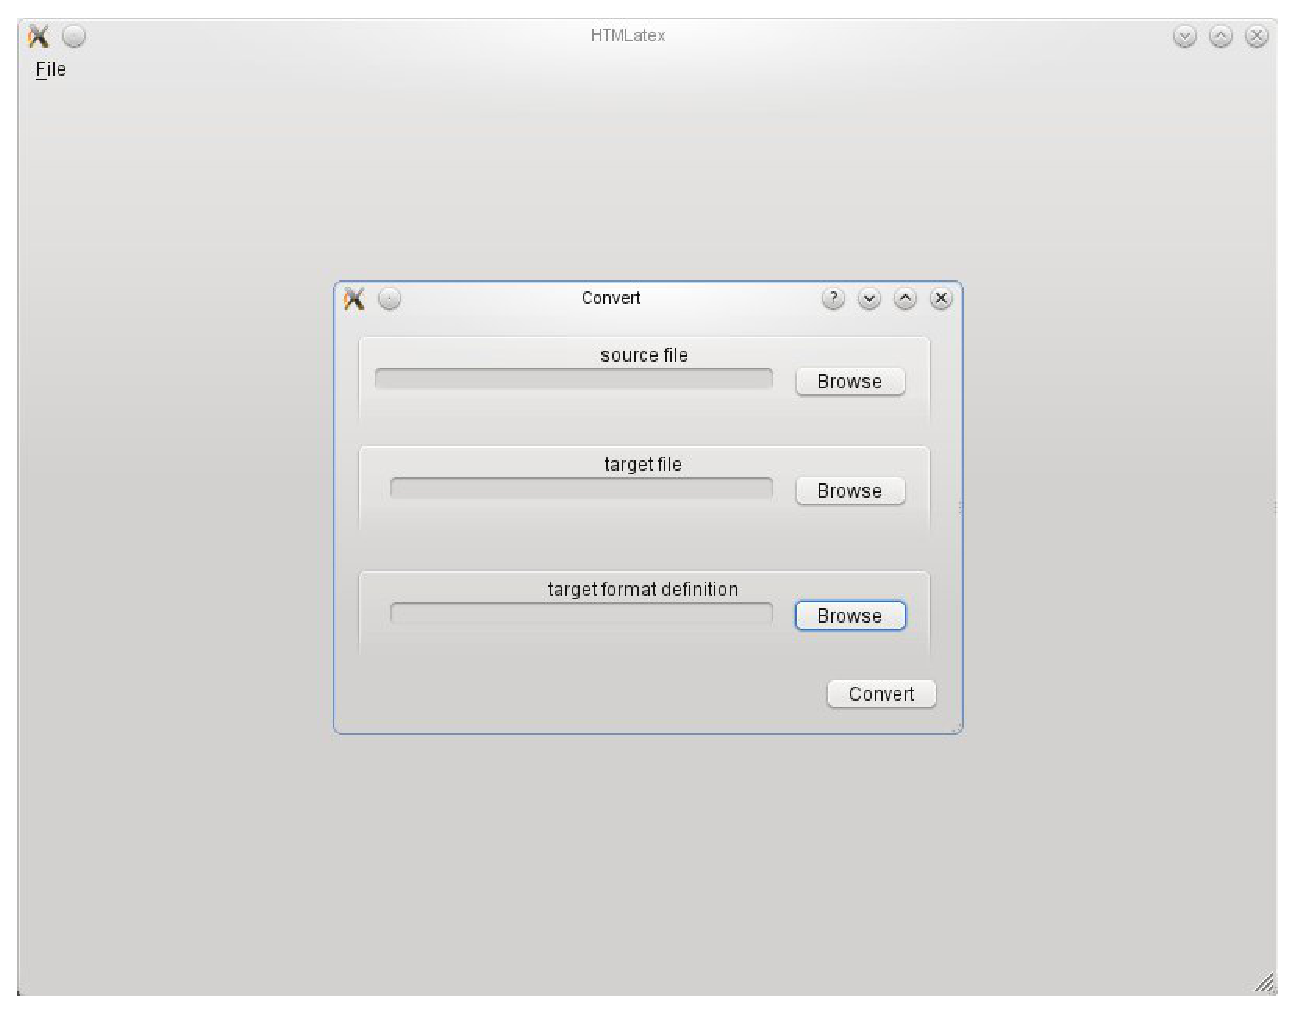
\includegraphics[width=.5\textwidth, keepaspectratio]{./img/screenshot.eps}
    \caption{BILDUNTERSCHRIFT}
\end{figure}

\section{Implementierung}
\begin{figure} [H]
\centering
\resizebox*{.70\textheight}{!}{%LaTeX with PSTricks extensions
%%Creator: inkscape 0.47
%%Please note this file requires PSTricks extensions
\psset{xunit=.5pt,yunit=.5pt,runit=.5pt}
\begin{pspicture}(739.99078369,308.8838501)
{
\newrgbcolor{curcolor}{0 0 0}
\pscustom[linestyle=none,fillstyle=solid,fillcolor=curcolor]
{
\newpath
\moveto(314.0554912,303.5983923)
\lineto(313.1424912,303.5983923)
\lineto(313.1424912,297.8343923)
\lineto(314.0554912,297.8343923)
\lineto(314.0554912,303.5983923)
\moveto(314.0554912,305.8533923)
\lineto(313.1314912,305.8533923)
\lineto(313.1314912,304.6983923)
\lineto(314.0554912,304.6983923)
\lineto(314.0554912,305.8533923)
}
}
{
\newrgbcolor{curcolor}{0 0 0}
\pscustom[linestyle=none,fillstyle=solid,fillcolor=curcolor]
{
\newpath
\moveto(315.62470995,303.5983923)
\lineto(315.62470995,297.8343923)
\lineto(316.54870995,297.8343923)
\lineto(316.54870995,301.0133923)
\curveto(316.54870995,302.19039112)(317.1647109,302.9603923)(318.11070995,302.9603923)
\curveto(318.83670923,302.9603923)(319.29870995,302.52039161)(319.29870995,301.8273923)
\lineto(319.29870995,297.8343923)
\lineto(320.21170995,297.8343923)
\lineto(320.21170995,302.1903923)
\curveto(320.21170995,303.14739134)(319.49670884,303.7633923)(318.38570995,303.7633923)
\curveto(317.52771081,303.7633923)(316.97770945,303.4333915)(316.47170995,302.6303923)
\lineto(316.47170995,303.5983923)
\lineto(315.62470995,303.5983923)
}
}
{
\newrgbcolor{curcolor}{0 0 0}
\pscustom[linestyle=none,fillstyle=solid,fillcolor=curcolor]
{
\newpath
\moveto(323.77175683,303.5983923)
\lineto(322.82575683,303.5983923)
\lineto(322.82575683,305.1823923)
\lineto(321.91275683,305.1823923)
\lineto(321.91275683,303.5983923)
\lineto(321.13175683,303.5983923)
\lineto(321.13175683,302.8503923)
\lineto(321.91275683,302.8503923)
\lineto(321.91275683,298.4943923)
\curveto(321.91275683,297.91139288)(322.30875754,297.5813923)(323.02375683,297.5813923)
\curveto(323.24375661,297.5813923)(323.46375714,297.60339235)(323.77175683,297.6583923)
\lineto(323.77175683,298.4283923)
\curveto(323.65075695,298.39539233)(323.50775665,298.3843923)(323.33175683,298.3843923)
\curveto(322.93575722,298.3843923)(322.82575683,298.49439271)(322.82575683,298.9013923)
\lineto(322.82575683,302.8503923)
\lineto(323.77175683,302.8503923)
\lineto(323.77175683,303.5983923)
}
}
{
\newrgbcolor{curcolor}{0 0 0}
\pscustom[linestyle=none,fillstyle=solid,fillcolor=curcolor]
{
\newpath
\moveto(329.67153808,300.4083923)
\curveto(329.67153808,301.28839142)(329.60553791,301.81639273)(329.44053808,302.2453923)
\curveto(329.06653845,303.19139135)(328.186537,303.7633923)(327.10853808,303.7633923)
\curveto(325.50253968,303.7633923)(324.46853808,302.53139041)(324.46853808,300.6393923)
\curveto(324.46853808,298.74739419)(325.46953969,297.5813923)(327.08653808,297.5813923)
\curveto(328.40653676,297.5813923)(329.31953831,298.32939355)(329.55053808,299.5833923)
\lineto(328.62653808,299.5833923)
\curveto(328.37353833,298.82439306)(327.85653734,298.4283923)(327.11953808,298.4283923)
\curveto(326.53653866,298.4283923)(326.04153777,298.69239278)(325.73353808,299.1763923)
\curveto(325.5135383,299.50639197)(325.43653807,299.83639287)(325.42553808,300.4083923)
\lineto(329.67153808,300.4083923)
\moveto(325.44753808,301.1563923)
\curveto(325.524538,302.22339123)(326.173539,302.9163923)(327.09753808,302.9163923)
\curveto(327.99953718,302.9163923)(328.69253808,302.16839135)(328.69253808,301.2223923)
\curveto(328.69253808,301.20039232)(328.69253807,301.17839228)(328.68153808,301.1563923)
\lineto(325.44753808,301.1563923)
}
}
{
\newrgbcolor{curcolor}{0 0 0}
\pscustom[linestyle=none,fillstyle=solid,fillcolor=curcolor]
{
\newpath
\moveto(330.91058495,303.5983923)
\lineto(330.91058495,297.8343923)
\lineto(331.83458495,297.8343923)
\lineto(331.83458495,300.8263923)
\curveto(331.83458495,301.65139147)(332.04358539,302.19039262)(332.48358495,302.5093923)
\curveto(332.76958467,302.71839209)(333.04458559,302.78439231)(333.68258495,302.7953923)
\lineto(333.68258495,303.7303923)
\curveto(333.52858511,303.75239228)(333.45158483,303.7633923)(333.33058495,303.7633923)
\curveto(332.73658555,303.7633923)(332.28558442,303.41139144)(331.75758495,302.5533923)
\lineto(331.75758495,303.5983923)
\lineto(330.91058495,303.5983923)
}
}
{
\newrgbcolor{curcolor}{0 0 0}
\pscustom[linestyle=none,fillstyle=solid,fillcolor=curcolor]
{
\newpath
\moveto(334.59541308,303.5983923)
\lineto(334.59541308,297.8343923)
\lineto(335.51941308,297.8343923)
\lineto(335.51941308,301.0133923)
\curveto(335.51941308,302.19039112)(336.13541402,302.9603923)(337.08141308,302.9603923)
\curveto(337.80741235,302.9603923)(338.26941308,302.52039161)(338.26941308,301.8273923)
\lineto(338.26941308,297.8343923)
\lineto(339.18241308,297.8343923)
\lineto(339.18241308,302.1903923)
\curveto(339.18241308,303.14739134)(338.46741197,303.7633923)(337.35641308,303.7633923)
\curveto(336.49841394,303.7633923)(335.94841257,303.4333915)(335.44241308,302.6303923)
\lineto(335.44241308,303.5983923)
\lineto(334.59541308,303.5983923)
}
}
{
\newrgbcolor{curcolor}{0 0 0}
\pscustom[linestyle=none,fillstyle=solid,fillcolor=curcolor]
{
\newpath
\moveto(345.59145995,300.4083923)
\curveto(345.59145995,301.28839142)(345.52545979,301.81639273)(345.36045995,302.2453923)
\curveto(344.98646033,303.19139135)(344.10645887,303.7633923)(343.02845995,303.7633923)
\curveto(341.42246156,303.7633923)(340.38845995,302.53139041)(340.38845995,300.6393923)
\curveto(340.38845995,298.74739419)(341.38946157,297.5813923)(343.00645995,297.5813923)
\curveto(344.32645863,297.5813923)(345.23946018,298.32939355)(345.47045995,299.5833923)
\lineto(344.54645995,299.5833923)
\curveto(344.29346021,298.82439306)(343.77645922,298.4283923)(343.03945995,298.4283923)
\curveto(342.45646054,298.4283923)(341.96145964,298.69239278)(341.65345995,299.1763923)
\curveto(341.43346017,299.50639197)(341.35645994,299.83639287)(341.34545995,300.4083923)
\lineto(345.59145995,300.4083923)
\moveto(341.36745995,301.1563923)
\curveto(341.44445988,302.22339123)(342.09346088,302.9163923)(343.01745995,302.9163923)
\curveto(343.91945905,302.9163923)(344.61245995,302.16839135)(344.61245995,301.2223923)
\curveto(344.61245995,301.20039232)(344.61245994,301.17839228)(344.60145995,301.1563923)
\lineto(341.36745995,301.1563923)
}
}
{
\newrgbcolor{curcolor}{0 0 0}
\pscustom[linestyle=none,fillstyle=solid,fillcolor=curcolor]
{
}
}
{
\newrgbcolor{curcolor}{0 0 0}
\pscustom[linestyle=none,fillstyle=solid,fillcolor=curcolor]
{
\newpath
\moveto(353.43428808,297.8343923)
\lineto(356.21728808,305.8533923)
\lineto(355.12828808,305.8533923)
\lineto(352.90628808,299.0663923)
\lineto(350.55228808,305.8533923)
\lineto(349.45228808,305.8533923)
\lineto(352.33428808,297.8343923)
\lineto(353.43428808,297.8343923)
}
}
{
\newrgbcolor{curcolor}{0 0 0}
\pscustom[linestyle=none,fillstyle=solid,fillcolor=curcolor]
{
\newpath
\moveto(362.11294433,300.4083923)
\curveto(362.11294433,301.28839142)(362.04694416,301.81639273)(361.88194433,302.2453923)
\curveto(361.5079447,303.19139135)(360.62794325,303.7633923)(359.54994433,303.7633923)
\curveto(357.94394593,303.7633923)(356.90994433,302.53139041)(356.90994433,300.6393923)
\curveto(356.90994433,298.74739419)(357.91094594,297.5813923)(359.52794433,297.5813923)
\curveto(360.84794301,297.5813923)(361.76094456,298.32939355)(361.99194433,299.5833923)
\lineto(361.06794433,299.5833923)
\curveto(360.81494458,298.82439306)(360.29794359,298.4283923)(359.56094433,298.4283923)
\curveto(358.97794491,298.4283923)(358.48294402,298.69239278)(358.17494433,299.1763923)
\curveto(357.95494455,299.50639197)(357.87794432,299.83639287)(357.86694433,300.4083923)
\lineto(362.11294433,300.4083923)
\moveto(357.88894433,301.1563923)
\curveto(357.96594425,302.22339123)(358.61494525,302.9163923)(359.53894433,302.9163923)
\curveto(360.44094343,302.9163923)(361.13394433,302.16839135)(361.13394433,301.2223923)
\curveto(361.13394433,301.20039232)(361.13394432,301.17839228)(361.12294433,301.1563923)
\lineto(357.88894433,301.1563923)
}
}
{
\newrgbcolor{curcolor}{0 0 0}
\pscustom[linestyle=none,fillstyle=solid,fillcolor=curcolor]
{
\newpath
\moveto(363.3519912,303.5983923)
\lineto(363.3519912,297.8343923)
\lineto(364.2759912,297.8343923)
\lineto(364.2759912,300.8263923)
\curveto(364.2759912,301.65139147)(364.48499164,302.19039262)(364.9249912,302.5093923)
\curveto(365.21099092,302.71839209)(365.48599184,302.78439231)(366.1239912,302.7953923)
\lineto(366.1239912,303.7303923)
\curveto(365.96999136,303.75239228)(365.89299108,303.7633923)(365.7719912,303.7633923)
\curveto(365.1779918,303.7633923)(364.72699067,303.41139144)(364.1989912,302.5533923)
\lineto(364.1989912,303.5983923)
\lineto(363.3519912,303.5983923)
}
}
{
\newrgbcolor{curcolor}{0 0 0}
\pscustom[linestyle=none,fillstyle=solid,fillcolor=curcolor]
{
\newpath
\moveto(372.15181933,298.3733923)
\curveto(372.05281943,298.35139232)(372.00881927,298.3513923)(371.95381933,298.3513923)
\curveto(371.63481965,298.3513923)(371.45881933,298.51639258)(371.45881933,298.8023923)
\lineto(371.45881933,302.1903923)
\curveto(371.45881933,303.21339128)(370.71081791,303.7633923)(369.29181933,303.7633923)
\curveto(368.45582016,303.7633923)(367.76281894,303.52139187)(367.37781933,303.0923923)
\curveto(367.11381959,302.7953926)(367.00381931,302.46539173)(366.98181933,301.8933923)
\lineto(367.90581933,301.8933923)
\curveto(367.98281925,302.59739159)(368.40082019,302.9163923)(369.25881933,302.9163923)
\curveto(370.0838185,302.9163923)(370.54581933,302.60839175)(370.54581933,302.0583923)
\lineto(370.54581933,301.8163923)
\curveto(370.54581933,301.43139268)(370.3148186,301.26639221)(369.58881933,301.1783923)
\curveto(368.29082063,301.01339246)(368.09281898,300.96939216)(367.74081933,300.8263923)
\curveto(367.06982,300.55139257)(366.72881933,300.03439155)(366.72881933,299.2863923)
\curveto(366.72881933,298.24139334)(367.45482049,297.5813923)(368.62081933,297.5813923)
\curveto(369.3468186,297.5813923)(369.92981998,297.83439289)(370.57881933,298.4283923)
\curveto(370.64481926,297.84539288)(370.93081992,297.5813923)(371.52481933,297.5813923)
\curveto(371.71181914,297.5813923)(371.85481962,297.60339238)(372.15181933,297.6803923)
\lineto(372.15181933,298.3733923)
\moveto(370.54581933,299.6493923)
\curveto(370.54581933,299.34139261)(370.45781905,299.15439205)(370.18281933,298.9013923)
\curveto(369.8088197,298.56039264)(369.35781879,298.3843923)(368.81881933,298.3843923)
\curveto(368.10382004,298.3843923)(367.68581933,298.72539288)(367.68581933,299.3083923)
\curveto(367.68581933,299.91339169)(368.09282031,300.22139244)(369.07181933,300.3643923)
\curveto(370.03981836,300.49639217)(370.23781964,300.54039244)(370.54581933,300.6833923)
\lineto(370.54581933,299.6493923)
}
}
{
\newrgbcolor{curcolor}{0 0 0}
\pscustom[linestyle=none,fillstyle=solid,fillcolor=curcolor]
{
\newpath
\moveto(373.1488662,303.5983923)
\lineto(373.1488662,297.8343923)
\lineto(374.0728662,297.8343923)
\lineto(374.0728662,300.8263923)
\curveto(374.0728662,301.65139147)(374.28186664,302.19039262)(374.7218662,302.5093923)
\curveto(375.00786592,302.71839209)(375.28286684,302.78439231)(375.9208662,302.7953923)
\lineto(375.9208662,303.7303923)
\curveto(375.76686636,303.75239228)(375.68986608,303.7633923)(375.5688662,303.7633923)
\curveto(374.9748668,303.7633923)(374.52386567,303.41139144)(373.9958662,302.5533923)
\lineto(373.9958662,303.5983923)
\lineto(373.1488662,303.5983923)
}
}
{
\newrgbcolor{curcolor}{0 0 0}
\pscustom[linestyle=none,fillstyle=solid,fillcolor=curcolor]
{
\newpath
\moveto(376.65769433,305.8533923)
\lineto(376.65769433,297.8343923)
\lineto(377.48269433,297.8343923)
\lineto(377.48269433,298.5713923)
\curveto(377.92269389,297.90039297)(378.50569513,297.5813923)(379.30869433,297.5813923)
\curveto(380.82669281,297.5813923)(381.81669433,298.82439421)(381.81669433,300.7383923)
\curveto(381.81669433,302.60839043)(380.87069281,303.7633923)(379.35269433,303.7633923)
\curveto(378.56069512,303.7633923)(377.9996939,303.46639165)(377.57069433,302.8173923)
\lineto(377.57069433,305.8533923)
\lineto(376.65769433,305.8533923)
\moveto(379.17669433,302.9053923)
\curveto(380.1996933,302.9053923)(380.85969433,302.01439092)(380.85969433,300.6393923)
\curveto(380.85969433,299.33039361)(380.17769333,298.4393923)(379.17669433,298.4393923)
\curveto(378.2086953,298.4393923)(377.57069433,299.31939365)(377.57069433,300.6723923)
\curveto(377.57069433,302.02539095)(378.2086953,302.9053923)(379.17669433,302.9053923)
}
}
{
\newrgbcolor{curcolor}{0 0 0}
\pscustom[linestyle=none,fillstyle=solid,fillcolor=curcolor]
{
\newpath
\moveto(387.8297412,300.4083923)
\curveto(387.8297412,301.28839142)(387.76374104,301.81639273)(387.5987412,302.2453923)
\curveto(387.22474158,303.19139135)(386.34474012,303.7633923)(385.2667412,303.7633923)
\curveto(383.66074281,303.7633923)(382.6267412,302.53139041)(382.6267412,300.6393923)
\curveto(382.6267412,298.74739419)(383.62774282,297.5813923)(385.2447412,297.5813923)
\curveto(386.56473988,297.5813923)(387.47774143,298.32939355)(387.7087412,299.5833923)
\lineto(386.7847412,299.5833923)
\curveto(386.53174146,298.82439306)(386.01474047,298.4283923)(385.2777412,298.4283923)
\curveto(384.69474179,298.4283923)(384.19974089,298.69239278)(383.8917412,299.1763923)
\curveto(383.67174142,299.50639197)(383.59474119,299.83639287)(383.5837412,300.4083923)
\lineto(387.8297412,300.4083923)
\moveto(383.6057412,301.1563923)
\curveto(383.68274113,302.22339123)(384.33174213,302.9163923)(385.2557412,302.9163923)
\curveto(386.1577403,302.9163923)(386.8507412,302.16839135)(386.8507412,301.2223923)
\curveto(386.8507412,301.20039232)(386.85074119,301.17839228)(386.8397412,301.1563923)
\lineto(383.6057412,301.1563923)
}
}
{
\newrgbcolor{curcolor}{0 0 0}
\pscustom[linestyle=none,fillstyle=solid,fillcolor=curcolor]
{
\newpath
\moveto(389.95978808,303.5983923)
\lineto(389.04678808,303.5983923)
\lineto(389.04678808,297.8343923)
\lineto(389.95978808,297.8343923)
\lineto(389.95978808,303.5983923)
\moveto(389.95978808,305.8533923)
\lineto(389.03578808,305.8533923)
\lineto(389.03578808,304.6983923)
\lineto(389.95978808,304.6983923)
\lineto(389.95978808,305.8533923)
}
}
{
\newrgbcolor{curcolor}{0 0 0}
\pscustom[linestyle=none,fillstyle=solid,fillcolor=curcolor]
{
\newpath
\moveto(393.55300683,303.5983923)
\lineto(392.60700683,303.5983923)
\lineto(392.60700683,305.1823923)
\lineto(391.69400683,305.1823923)
\lineto(391.69400683,303.5983923)
\lineto(390.91300683,303.5983923)
\lineto(390.91300683,302.8503923)
\lineto(391.69400683,302.8503923)
\lineto(391.69400683,298.4943923)
\curveto(391.69400683,297.91139288)(392.09000754,297.5813923)(392.80500683,297.5813923)
\curveto(393.02500661,297.5813923)(393.24500714,297.60339235)(393.55300683,297.6583923)
\lineto(393.55300683,298.4283923)
\curveto(393.43200695,298.39539233)(393.28900665,298.3843923)(393.11300683,298.3843923)
\curveto(392.71700722,298.3843923)(392.60700683,298.49439271)(392.60700683,298.9013923)
\lineto(392.60700683,302.8503923)
\lineto(393.55300683,302.8503923)
\lineto(393.55300683,303.5983923)
}
}
{
\newrgbcolor{curcolor}{0 0 0}
\pscustom[linestyle=none,fillstyle=solid,fillcolor=curcolor]
{
\newpath
\moveto(399.11178808,297.8343923)
\lineto(399.11178808,303.5983923)
\lineto(398.19878808,303.5983923)
\lineto(398.19878808,300.3313923)
\curveto(398.19878808,299.15439348)(397.58278712,298.3843923)(396.62578808,298.3843923)
\curveto(395.8997888,298.3843923)(395.43778808,298.82439299)(395.43778808,299.5173923)
\lineto(395.43778808,303.5983923)
\lineto(394.52478808,303.5983923)
\lineto(394.52478808,299.1543923)
\curveto(394.52478808,298.19739326)(395.2397892,297.5813923)(396.36178808,297.5813923)
\curveto(397.20878723,297.5813923)(397.74778862,297.87839306)(398.28678808,298.6373923)
\lineto(398.28678808,297.8343923)
\lineto(399.11178808,297.8343923)
}
}
{
\newrgbcolor{curcolor}{0 0 0}
\pscustom[linestyle=none,fillstyle=solid,fillcolor=curcolor]
{
\newpath
\moveto(400.70283495,303.5983923)
\lineto(400.70283495,297.8343923)
\lineto(401.62683495,297.8343923)
\lineto(401.62683495,301.0133923)
\curveto(401.62683495,302.19039112)(402.2428359,302.9603923)(403.18883495,302.9603923)
\curveto(403.91483423,302.9603923)(404.37683495,302.52039161)(404.37683495,301.8273923)
\lineto(404.37683495,297.8343923)
\lineto(405.28983495,297.8343923)
\lineto(405.28983495,302.1903923)
\curveto(405.28983495,303.14739134)(404.57483384,303.7633923)(403.46383495,303.7633923)
\curveto(402.60583581,303.7633923)(402.05583445,303.4333915)(401.54983495,302.6303923)
\lineto(401.54983495,303.5983923)
\lineto(400.70283495,303.5983923)
}
}
{
\newrgbcolor{curcolor}{0 0 0}
\pscustom[linestyle=none,fillstyle=solid,fillcolor=curcolor]
{
\newpath
\moveto(410.58788183,303.5983923)
\lineto(410.58788183,302.7623923)
\curveto(410.12588229,303.44439162)(409.56488109,303.7633923)(408.82788183,303.7633923)
\curveto(407.36488329,303.7633923)(406.37488183,302.48739043)(406.37488183,300.6173923)
\curveto(406.37488183,299.67139324)(406.6278823,298.90139175)(407.10088183,298.3513923)
\curveto(407.5298814,297.86739278)(408.14588243,297.5813923)(408.75088183,297.5813923)
\curveto(409.4768811,297.5813923)(409.98288234,297.88939302)(410.49988183,298.6153923)
\lineto(410.49988183,298.3183923)
\curveto(410.49988183,297.53739308)(410.4008816,297.06439198)(410.16988183,296.7453923)
\curveto(409.92788207,296.40439264)(409.45488127,296.2063923)(408.89388183,296.2063923)
\curveto(408.47588225,296.2063923)(408.10188157,296.3163925)(407.84888183,296.5143923)
\curveto(407.63988204,296.67939213)(407.55188177,296.83339264)(407.49688183,297.1743923)
\lineto(406.56188183,297.1743923)
\curveto(406.66088173,296.08539339)(407.50788318,295.4363923)(408.86088183,295.4363923)
\curveto(409.71888097,295.4363923)(410.4558822,295.71139276)(410.82988183,296.1733923)
\curveto(411.26988139,296.70139177)(411.43488183,297.42739365)(411.43488183,298.7803923)
\lineto(411.43488183,303.5983923)
\lineto(410.58788183,303.5983923)
\moveto(408.92688183,302.9163923)
\curveto(409.91688084,302.9163923)(410.49988183,302.08039086)(410.49988183,300.6393923)
\curveto(410.49988183,299.26439367)(409.90588086,298.4283923)(408.93788183,298.4283923)
\curveto(407.93688283,298.4283923)(407.33188183,299.2753937)(407.33188183,300.6723923)
\curveto(407.33188183,302.05839091)(407.94788281,302.9163923)(408.92688183,302.9163923)
}
}
{
\newrgbcolor{curcolor}{0 0 0}
\pscustom[linestyle=none,fillstyle=solid,fillcolor=curcolor]
{
\newpath
\moveto(18.18273495,302.4965448)
\lineto(22.54973495,302.4965448)
\lineto(22.54973495,303.3985448)
\lineto(18.18273495,303.3985448)
\lineto(18.18273495,305.9615448)
\lineto(22.71473495,305.9615448)
\lineto(22.71473495,306.8635448)
\lineto(17.15973495,306.8635448)
\lineto(17.15973495,298.8445448)
\lineto(22.91273495,298.8445448)
\lineto(22.91273495,299.7465448)
\lineto(18.18273495,299.7465448)
\lineto(18.18273495,302.4965448)
}
}
{
\newrgbcolor{curcolor}{0 0 0}
\pscustom[linestyle=none,fillstyle=solid,fillcolor=curcolor]
{
\newpath
\moveto(25.1673912,304.6085448)
\lineto(24.2543912,304.6085448)
\lineto(24.2543912,298.8445448)
\lineto(25.1673912,298.8445448)
\lineto(25.1673912,304.6085448)
\moveto(25.1673912,306.8635448)
\lineto(24.2433912,306.8635448)
\lineto(24.2433912,305.7085448)
\lineto(25.1673912,305.7085448)
\lineto(25.1673912,306.8635448)
}
}
{
\newrgbcolor{curcolor}{0 0 0}
\pscustom[linestyle=none,fillstyle=solid,fillcolor=curcolor]
{
\newpath
\moveto(26.73660995,304.6085448)
\lineto(26.73660995,298.8445448)
\lineto(27.66060995,298.8445448)
\lineto(27.66060995,302.0235448)
\curveto(27.66060995,303.20054362)(28.2766109,303.9705448)(29.22260995,303.9705448)
\curveto(29.94860923,303.9705448)(30.41060995,303.53054411)(30.41060995,302.8375448)
\lineto(30.41060995,298.8445448)
\lineto(31.32360995,298.8445448)
\lineto(31.32360995,303.2005448)
\curveto(31.32360995,304.15754384)(30.60860884,304.7735448)(29.49760995,304.7735448)
\curveto(28.63961081,304.7735448)(28.08960945,304.443544)(27.58360995,303.6405448)
\lineto(27.58360995,304.6085448)
\lineto(26.73660995,304.6085448)
}
}
{
\newrgbcolor{curcolor}{0 0 0}
\pscustom[linestyle=none,fillstyle=solid,fillcolor=curcolor]
{
\newpath
\moveto(36.62165683,304.6085448)
\lineto(36.62165683,303.7725448)
\curveto(36.15965729,304.45454412)(35.59865609,304.7735448)(34.86165683,304.7735448)
\curveto(33.39865829,304.7735448)(32.40865683,303.49754293)(32.40865683,301.6275448)
\curveto(32.40865683,300.68154574)(32.6616573,299.91154425)(33.13465683,299.3615448)
\curveto(33.5636564,298.87754528)(34.17965743,298.5915448)(34.78465683,298.5915448)
\curveto(35.5106561,298.5915448)(36.01665734,298.89954552)(36.53365683,299.6255448)
\lineto(36.53365683,299.3285448)
\curveto(36.53365683,298.54754558)(36.4346566,298.07454448)(36.20365683,297.7555448)
\curveto(35.96165707,297.41454514)(35.48865627,297.2165448)(34.92765683,297.2165448)
\curveto(34.50965725,297.2165448)(34.13565657,297.326545)(33.88265683,297.5245448)
\curveto(33.67365704,297.68954463)(33.58565677,297.84354514)(33.53065683,298.1845448)
\lineto(32.59565683,298.1845448)
\curveto(32.69465673,297.09554589)(33.54165818,296.4465448)(34.89465683,296.4465448)
\curveto(35.75265597,296.4465448)(36.4896572,296.72154526)(36.86365683,297.1835448)
\curveto(37.30365639,297.71154427)(37.46865683,298.43754615)(37.46865683,299.7905448)
\lineto(37.46865683,304.6085448)
\lineto(36.62165683,304.6085448)
\moveto(34.96065683,303.9265448)
\curveto(35.95065584,303.9265448)(36.53365683,303.09054336)(36.53365683,301.6495448)
\curveto(36.53365683,300.27454617)(35.93965586,299.4385448)(34.97165683,299.4385448)
\curveto(33.97065783,299.4385448)(33.36565683,300.2855462)(33.36565683,301.6825448)
\curveto(33.36565683,303.06854341)(33.98165781,303.9265448)(34.96065683,303.9265448)
}
}
{
\newrgbcolor{curcolor}{0 0 0}
\pscustom[linestyle=none,fillstyle=solid,fillcolor=curcolor]
{
\newpath
\moveto(44.0977037,299.3835448)
\curveto(43.9987038,299.36154482)(43.95470365,299.3615448)(43.8997037,299.3615448)
\curveto(43.58070402,299.3615448)(43.4047037,299.52654508)(43.4047037,299.8125448)
\lineto(43.4047037,303.2005448)
\curveto(43.4047037,304.22354378)(42.65670228,304.7735448)(41.2377037,304.7735448)
\curveto(40.40170454,304.7735448)(39.70870332,304.53154437)(39.3237037,304.1025448)
\curveto(39.05970397,303.8055451)(38.94970368,303.47554423)(38.9277037,302.9035448)
\lineto(39.8517037,302.9035448)
\curveto(39.92870363,303.60754409)(40.34670456,303.9265448)(41.2047037,303.9265448)
\curveto(42.02970288,303.9265448)(42.4917037,303.61854425)(42.4917037,303.0685448)
\lineto(42.4917037,302.8265448)
\curveto(42.4917037,302.44154518)(42.26070298,302.27654471)(41.5347037,302.1885448)
\curveto(40.236705,302.02354496)(40.03870335,301.97954466)(39.6867037,301.8365448)
\curveto(39.01570437,301.56154507)(38.6747037,301.04454405)(38.6747037,300.2965448)
\curveto(38.6747037,299.25154584)(39.40070487,298.5915448)(40.5667037,298.5915448)
\curveto(41.29270298,298.5915448)(41.87570435,298.84454539)(42.5247037,299.4385448)
\curveto(42.59070364,298.85554538)(42.8767043,298.5915448)(43.4707037,298.5915448)
\curveto(43.65770352,298.5915448)(43.800704,298.61354488)(44.0977037,298.6905448)
\lineto(44.0977037,299.3835448)
\moveto(42.4917037,300.6595448)
\curveto(42.4917037,300.35154511)(42.40370343,300.16454455)(42.1287037,299.9115448)
\curveto(41.75470408,299.57054514)(41.30370316,299.3945448)(40.7647037,299.3945448)
\curveto(40.04970442,299.3945448)(39.6317037,299.73554538)(39.6317037,300.3185448)
\curveto(39.6317037,300.92354419)(40.03870468,301.23154494)(41.0177037,301.3745448)
\curveto(41.98570273,301.50654467)(42.18370401,301.55054494)(42.4917037,301.6935448)
\lineto(42.4917037,300.6595448)
}
}
{
\newrgbcolor{curcolor}{0 0 0}
\pscustom[linestyle=none,fillstyle=solid,fillcolor=curcolor]
{
\newpath
\moveto(44.92975058,306.8635448)
\lineto(44.92975058,298.8445448)
\lineto(45.75475058,298.8445448)
\lineto(45.75475058,299.5815448)
\curveto(46.19475014,298.91054547)(46.77775138,298.5915448)(47.58075058,298.5915448)
\curveto(49.09874906,298.5915448)(50.08875058,299.83454671)(50.08875058,301.7485448)
\curveto(50.08875058,303.61854293)(49.14274906,304.7735448)(47.62475058,304.7735448)
\curveto(46.83275137,304.7735448)(46.27175015,304.47654415)(45.84275058,303.8275448)
\lineto(45.84275058,306.8635448)
\lineto(44.92975058,306.8635448)
\moveto(47.44875058,303.9155448)
\curveto(48.47174955,303.9155448)(49.13175058,303.02454342)(49.13175058,301.6495448)
\curveto(49.13175058,300.34054611)(48.44974958,299.4495448)(47.44875058,299.4495448)
\curveto(46.48075155,299.4495448)(45.84275058,300.32954615)(45.84275058,301.6825448)
\curveto(45.84275058,303.03554345)(46.48075155,303.9155448)(47.44875058,303.9155448)
}
}
{
\newrgbcolor{curcolor}{0 0 0}
\pscustom[linestyle=none,fillstyle=solid,fillcolor=curcolor]
{
\newpath
\moveto(56.10179745,301.4185448)
\curveto(56.10179745,302.29854392)(56.03579729,302.82654523)(55.87079745,303.2555448)
\curveto(55.49679783,304.20154385)(54.61679637,304.7735448)(53.53879745,304.7735448)
\curveto(51.93279906,304.7735448)(50.89879745,303.54154291)(50.89879745,301.6495448)
\curveto(50.89879745,299.75754669)(51.89979907,298.5915448)(53.51679745,298.5915448)
\curveto(54.83679613,298.5915448)(55.74979768,299.33954605)(55.98079745,300.5935448)
\lineto(55.05679745,300.5935448)
\curveto(54.80379771,299.83454556)(54.28679672,299.4385448)(53.54979745,299.4385448)
\curveto(52.96679804,299.4385448)(52.47179714,299.70254528)(52.16379745,300.1865448)
\curveto(51.94379767,300.51654447)(51.86679744,300.84654537)(51.85579745,301.4185448)
\lineto(56.10179745,301.4185448)
\moveto(51.87779745,302.1665448)
\curveto(51.95479738,303.23354373)(52.60379838,303.9265448)(53.52779745,303.9265448)
\curveto(54.42979655,303.9265448)(55.12279745,303.17854385)(55.12279745,302.2325448)
\curveto(55.12279745,302.21054482)(55.12279744,302.18854478)(55.11179745,302.1665448)
\lineto(51.87779745,302.1665448)
}
}
{
\newrgbcolor{curcolor}{0 0 0}
\pscustom[linestyle=none,fillstyle=solid,fillcolor=curcolor]
{
\newpath
\moveto(58.93584433,299.9885448)
\lineto(57.79184433,299.9885448)
\lineto(57.79184433,298.8445448)
\lineto(58.93584433,298.8445448)
\lineto(58.93584433,299.9885448)
\moveto(58.93584433,304.6085448)
\lineto(57.79184433,304.6085448)
\lineto(57.79184433,303.4645448)
\lineto(58.93584433,303.4645448)
\lineto(58.93584433,304.6085448)
}
}
{
\newrgbcolor{curcolor}{0 0 0}
\pscustom[linestyle=none,fillstyle=solid,fillcolor=curcolor]
{
}
}
{
\newrgbcolor{curcolor}{0 0 0}
\pscustom[linestyle=none,fillstyle=solid,fillcolor=curcolor]
{
\newpath
\moveto(66.34640683,306.8635448)
\lineto(66.34640683,301.2205448)
\curveto(66.34640683,300.58254544)(66.28040664,300.21954452)(66.09340683,299.9445448)
\curveto(65.89540703,299.63654511)(65.52140642,299.4495448)(65.11440683,299.4495448)
\curveto(64.3444076,299.4495448)(63.91540683,299.96654573)(63.91540683,300.9015448)
\lineto(63.91540683,301.4185448)
\lineto(62.87040683,301.4185448)
\lineto(62.87040683,300.7145448)
\curveto(62.87040683,299.4165461)(63.7284082,298.5915448)(65.10340683,298.5915448)
\curveto(66.50040543,298.5915448)(67.36940683,299.46054618)(67.36940683,300.8465448)
\lineto(67.36940683,306.8635448)
\lineto(66.34640683,306.8635448)
}
}
{
\newrgbcolor{curcolor}{0 0 0}
\pscustom[linestyle=none,fillstyle=solid,fillcolor=curcolor]
{
\newpath
\moveto(74.06840683,299.3835448)
\curveto(73.96940693,299.36154482)(73.92540677,299.3615448)(73.87040683,299.3615448)
\curveto(73.55140715,299.3615448)(73.37540683,299.52654508)(73.37540683,299.8125448)
\lineto(73.37540683,303.2005448)
\curveto(73.37540683,304.22354378)(72.62740541,304.7735448)(71.20840683,304.7735448)
\curveto(70.37240766,304.7735448)(69.67940644,304.53154437)(69.29440683,304.1025448)
\curveto(69.03040709,303.8055451)(68.92040681,303.47554423)(68.89840683,302.9035448)
\lineto(69.82240683,302.9035448)
\curveto(69.89940675,303.60754409)(70.31740769,303.9265448)(71.17540683,303.9265448)
\curveto(72.000406,303.9265448)(72.46240683,303.61854425)(72.46240683,303.0685448)
\lineto(72.46240683,302.8265448)
\curveto(72.46240683,302.44154518)(72.2314061,302.27654471)(71.50540683,302.1885448)
\curveto(70.20740813,302.02354496)(70.00940648,301.97954466)(69.65740683,301.8365448)
\curveto(68.9864075,301.56154507)(68.64540683,301.04454405)(68.64540683,300.2965448)
\curveto(68.64540683,299.25154584)(69.37140799,298.5915448)(70.53740683,298.5915448)
\curveto(71.2634061,298.5915448)(71.84640748,298.84454539)(72.49540683,299.4385448)
\curveto(72.56140676,298.85554538)(72.84740742,298.5915448)(73.44140683,298.5915448)
\curveto(73.62840664,298.5915448)(73.77140712,298.61354488)(74.06840683,298.6905448)
\lineto(74.06840683,299.3835448)
\moveto(72.46240683,300.6595448)
\curveto(72.46240683,300.35154511)(72.37440655,300.16454455)(72.09940683,299.9115448)
\curveto(71.7254072,299.57054514)(71.27440629,299.3945448)(70.73540683,299.3945448)
\curveto(70.02040754,299.3945448)(69.60240683,299.73554538)(69.60240683,300.3185448)
\curveto(69.60240683,300.92354419)(70.00940781,301.23154494)(70.98840683,301.3745448)
\curveto(71.95640586,301.50654467)(72.15440714,301.55054494)(72.46240683,301.6935448)
\lineto(72.46240683,300.6595448)
}
}
{
\newrgbcolor{curcolor}{0 0 0}
\pscustom[linestyle=none,fillstyle=solid,fillcolor=curcolor]
{
\newpath
\moveto(77.4414537,298.8445448)
\lineto(79.6524537,304.6085448)
\lineto(78.6184537,304.6085448)
\lineto(76.9904537,299.9335448)
\lineto(75.4504537,304.6085448)
\lineto(74.4164537,304.6085448)
\lineto(76.4404537,298.8445448)
\lineto(77.4414537,298.8445448)
}
}
{
\newrgbcolor{curcolor}{0 0 0}
\pscustom[linestyle=none,fillstyle=solid,fillcolor=curcolor]
{
\newpath
\moveto(85.6914537,299.3835448)
\curveto(85.5924538,299.36154482)(85.54845365,299.3615448)(85.4934537,299.3615448)
\curveto(85.17445402,299.3615448)(84.9984537,299.52654508)(84.9984537,299.8125448)
\lineto(84.9984537,303.2005448)
\curveto(84.9984537,304.22354378)(84.25045228,304.7735448)(82.8314537,304.7735448)
\curveto(81.99545454,304.7735448)(81.30245332,304.53154437)(80.9174537,304.1025448)
\curveto(80.65345397,303.8055451)(80.54345368,303.47554423)(80.5214537,302.9035448)
\lineto(81.4454537,302.9035448)
\curveto(81.52245363,303.60754409)(81.94045456,303.9265448)(82.7984537,303.9265448)
\curveto(83.62345288,303.9265448)(84.0854537,303.61854425)(84.0854537,303.0685448)
\lineto(84.0854537,302.8265448)
\curveto(84.0854537,302.44154518)(83.85445298,302.27654471)(83.1284537,302.1885448)
\curveto(81.830455,302.02354496)(81.63245335,301.97954466)(81.2804537,301.8365448)
\curveto(80.60945437,301.56154507)(80.2684537,301.04454405)(80.2684537,300.2965448)
\curveto(80.2684537,299.25154584)(80.99445487,298.5915448)(82.1604537,298.5915448)
\curveto(82.88645298,298.5915448)(83.46945435,298.84454539)(84.1184537,299.4385448)
\curveto(84.18445364,298.85554538)(84.4704543,298.5915448)(85.0644537,298.5915448)
\curveto(85.25145352,298.5915448)(85.394454,298.61354488)(85.6914537,298.6905448)
\lineto(85.6914537,299.3835448)
\moveto(84.0854537,300.6595448)
\curveto(84.0854537,300.35154511)(83.99745343,300.16454455)(83.7224537,299.9115448)
\curveto(83.34845408,299.57054514)(82.89745316,299.3945448)(82.3584537,299.3945448)
\curveto(81.64345442,299.3945448)(81.2254537,299.73554538)(81.2254537,300.3185448)
\curveto(81.2254537,300.92354419)(81.63245468,301.23154494)(82.6114537,301.3745448)
\curveto(83.57945273,301.50654467)(83.77745401,301.55054494)(84.0854537,301.6935448)
\lineto(84.0854537,300.6595448)
}
}
{
\newrgbcolor{curcolor}{0 0 0}
\pscustom[linestyle=none,fillstyle=solid,fillcolor=curcolor]
{
\newpath
\moveto(91.37450058,306.8635448)
\lineto(90.46150058,306.8635448)
\lineto(90.46150058,303.8825448)
\curveto(90.07650096,304.46554422)(89.46049981,304.7735448)(88.69050058,304.7735448)
\curveto(87.19450207,304.7735448)(86.21550058,303.57454296)(86.21550058,301.7375448)
\curveto(86.21550058,299.79054675)(87.17250213,298.5915448)(88.72350058,298.5915448)
\curveto(89.51549979,298.5915448)(90.06550107,298.88854551)(90.56050058,299.6035448)
\lineto(90.56050058,298.8445448)
\lineto(91.37450058,298.8445448)
\lineto(91.37450058,306.8635448)
\moveto(88.84450058,303.9155448)
\curveto(89.83449959,303.9155448)(90.46150058,303.03554342)(90.46150058,301.6605448)
\curveto(90.46150058,300.32954613)(89.82349961,299.4495448)(88.85550058,299.4495448)
\curveto(87.84350159,299.4495448)(87.17250058,300.34054614)(87.17250058,301.6825448)
\curveto(87.17250058,303.02454346)(87.84350158,303.9155448)(88.84450058,303.9155448)
}
}
{
\newrgbcolor{curcolor}{0 0 0}
\pscustom[linestyle=none,fillstyle=solid,fillcolor=curcolor]
{
\newpath
\moveto(95.04454745,304.7735448)
\curveto(93.42754907,304.7735448)(92.44854745,303.61854286)(92.44854745,301.6825448)
\curveto(92.44854745,299.74654673)(93.41654909,298.5915448)(95.05554745,298.5915448)
\curveto(96.67254584,298.5915448)(97.66254745,299.74654669)(97.66254745,301.6385448)
\curveto(97.66254745,303.62954281)(96.70554579,304.7735448)(95.04454745,304.7735448)
\moveto(95.05554745,303.9265448)
\curveto(96.08954642,303.9265448)(96.70554745,303.07954337)(96.70554745,301.6495448)
\curveto(96.70554745,300.29654615)(96.06754644,299.4385448)(95.05554745,299.4385448)
\curveto(94.03254848,299.4385448)(93.40554745,300.2855462)(93.40554745,301.6825448)
\curveto(93.40554745,303.06854341)(94.03254848,303.9265448)(95.05554745,303.9265448)
}
}
{
\newrgbcolor{curcolor}{0 0 0}
\pscustom[linestyle=none,fillstyle=solid,fillcolor=curcolor]
{
\newpath
\moveto(103.35659433,302.6725448)
\curveto(103.31259437,303.23354424)(103.19159411,303.59654512)(102.97159433,303.9155448)
\curveto(102.57559472,304.45454426)(101.88259352,304.7735448)(101.07959433,304.7735448)
\curveto(99.52859588,304.7735448)(98.51659433,303.54154288)(98.51659433,301.6275448)
\curveto(98.51659433,299.76854666)(99.50659589,298.5915448)(101.06859433,298.5915448)
\curveto(102.44359295,298.5915448)(103.31259444,299.41654621)(103.42259433,300.8245448)
\lineto(102.49859433,300.8245448)
\curveto(102.34459448,299.90054572)(101.87159355,299.4385448)(101.09059433,299.4385448)
\curveto(100.07859534,299.4385448)(99.47359433,300.26354616)(99.47359433,301.6275448)
\curveto(99.47359433,303.06854336)(100.06759533,303.9265448)(101.06859433,303.9265448)
\curveto(101.83859356,303.9265448)(102.32259444,303.475544)(102.43259433,302.6725448)
\lineto(103.35659433,302.6725448)
}
}
{
\newrgbcolor{curcolor}{0 0 0}
\pscustom[linestyle=none,fillstyle=solid,fillcolor=curcolor]
{
\newpath
\moveto(106.79959433,302.2765448)
\lineto(104.18159433,302.2765448)
\lineto(104.18159433,301.4845448)
\lineto(106.79959433,301.4845448)
\lineto(106.79959433,302.2765448)
}
}
{
\newrgbcolor{curcolor}{0 0 0}
\pscustom[linestyle=none,fillstyle=solid,fillcolor=curcolor]
{
\newpath
\moveto(111.88142245,304.6085448)
\lineto(111.88142245,303.7725448)
\curveto(111.41942291,304.45454412)(110.85842172,304.7735448)(110.12142245,304.7735448)
\curveto(108.65842392,304.7735448)(107.66842245,303.49754293)(107.66842245,301.6275448)
\curveto(107.66842245,300.68154574)(107.92142293,299.91154425)(108.39442245,299.3615448)
\curveto(108.82342202,298.87754528)(109.43942306,298.5915448)(110.04442245,298.5915448)
\curveto(110.77042173,298.5915448)(111.27642297,298.89954552)(111.79342245,299.6255448)
\lineto(111.79342245,299.3285448)
\curveto(111.79342245,298.54754558)(111.69442222,298.07454448)(111.46342245,297.7555448)
\curveto(111.22142269,297.41454514)(110.74842189,297.2165448)(110.18742245,297.2165448)
\curveto(109.76942287,297.2165448)(109.3954222,297.326545)(109.14242245,297.5245448)
\curveto(108.93342266,297.68954463)(108.8454224,297.84354514)(108.79042245,298.1845448)
\lineto(107.85542245,298.1845448)
\curveto(107.95442235,297.09554589)(108.80142381,296.4465448)(110.15442245,296.4465448)
\curveto(111.01242159,296.4465448)(111.74942283,296.72154526)(112.12342245,297.1835448)
\curveto(112.56342201,297.71154427)(112.72842245,298.43754615)(112.72842245,299.7905448)
\lineto(112.72842245,304.6085448)
\lineto(111.88142245,304.6085448)
\moveto(110.22042245,303.9265448)
\curveto(111.21042146,303.9265448)(111.79342245,303.09054336)(111.79342245,301.6495448)
\curveto(111.79342245,300.27454617)(111.19942148,299.4385448)(110.23142245,299.4385448)
\curveto(109.23042345,299.4385448)(108.62542245,300.2855462)(108.62542245,301.6825448)
\curveto(108.62542245,303.06854341)(109.24142343,303.9265448)(110.22042245,303.9265448)
}
}
{
\newrgbcolor{curcolor}{0 0 0}
\pscustom[linestyle=none,fillstyle=solid,fillcolor=curcolor]
{
\newpath
\moveto(119.11546933,301.4185448)
\curveto(119.11546933,302.29854392)(119.04946916,302.82654523)(118.88446933,303.2555448)
\curveto(118.5104697,304.20154385)(117.63046825,304.7735448)(116.55246933,304.7735448)
\curveto(114.94647093,304.7735448)(113.91246933,303.54154291)(113.91246933,301.6495448)
\curveto(113.91246933,299.75754669)(114.91347094,298.5915448)(116.53046933,298.5915448)
\curveto(117.85046801,298.5915448)(118.76346956,299.33954605)(118.99446933,300.5935448)
\lineto(118.07046933,300.5935448)
\curveto(117.81746958,299.83454556)(117.30046859,299.4385448)(116.56346933,299.4385448)
\curveto(115.98046991,299.4385448)(115.48546902,299.70254528)(115.17746933,300.1865448)
\curveto(114.95746955,300.51654447)(114.88046932,300.84654537)(114.86946933,301.4185448)
\lineto(119.11546933,301.4185448)
\moveto(114.89146933,302.1665448)
\curveto(114.96846925,303.23354373)(115.61747025,303.9265448)(116.54146933,303.9265448)
\curveto(117.44346843,303.9265448)(118.13646933,303.17854385)(118.13646933,302.2325448)
\curveto(118.13646933,302.21054482)(118.13646932,302.18854478)(118.12546933,302.1665448)
\lineto(114.89146933,302.1665448)
}
}
{
\newrgbcolor{curcolor}{0 0 0}
\pscustom[linestyle=none,fillstyle=solid,fillcolor=curcolor]
{
\newpath
\moveto(120.3655162,304.6085448)
\lineto(120.3655162,298.8445448)
\lineto(121.2895162,298.8445448)
\lineto(121.2895162,302.0235448)
\curveto(121.2895162,303.20054362)(121.90551715,303.9705448)(122.8515162,303.9705448)
\curveto(123.57751548,303.9705448)(124.0395162,303.53054411)(124.0395162,302.8375448)
\lineto(124.0395162,298.8445448)
\lineto(124.9525162,298.8445448)
\lineto(124.9525162,303.2005448)
\curveto(124.9525162,304.15754384)(124.23751509,304.7735448)(123.1265162,304.7735448)
\curveto(122.26851706,304.7735448)(121.7185157,304.443544)(121.2125162,303.6405448)
\lineto(121.2125162,304.6085448)
\lineto(120.3655162,304.6085448)
}
}
{
\newrgbcolor{curcolor}{0 0 0}
\pscustom[linestyle=none,fillstyle=solid,fillcolor=curcolor]
{
\newpath
\moveto(131.36156308,301.4185448)
\curveto(131.36156308,302.29854392)(131.29556291,302.82654523)(131.13056308,303.2555448)
\curveto(130.75656345,304.20154385)(129.876562,304.7735448)(128.79856308,304.7735448)
\curveto(127.19256468,304.7735448)(126.15856308,303.54154291)(126.15856308,301.6495448)
\curveto(126.15856308,299.75754669)(127.15956469,298.5915448)(128.77656308,298.5915448)
\curveto(130.09656176,298.5915448)(131.00956331,299.33954605)(131.24056308,300.5935448)
\lineto(130.31656308,300.5935448)
\curveto(130.06356333,299.83454556)(129.54656234,299.4385448)(128.80956308,299.4385448)
\curveto(128.22656366,299.4385448)(127.73156277,299.70254528)(127.42356308,300.1865448)
\curveto(127.2035633,300.51654447)(127.12656307,300.84654537)(127.11556308,301.4185448)
\lineto(131.36156308,301.4185448)
\moveto(127.13756308,302.1665448)
\curveto(127.214563,303.23354373)(127.863564,303.9265448)(128.78756308,303.9265448)
\curveto(129.68956218,303.9265448)(130.38256308,303.17854385)(130.38256308,302.2325448)
\curveto(130.38256308,302.21054482)(130.38256307,302.18854478)(130.37156308,302.1665448)
\lineto(127.13756308,302.1665448)
}
}
{
\newrgbcolor{curcolor}{0 0 0}
\pscustom[linestyle=none,fillstyle=solid,fillcolor=curcolor]
{
\newpath
\moveto(132.60060995,304.6085448)
\lineto(132.60060995,298.8445448)
\lineto(133.52460995,298.8445448)
\lineto(133.52460995,301.8365448)
\curveto(133.52460995,302.66154397)(133.73361039,303.20054512)(134.17360995,303.5195448)
\curveto(134.45960967,303.72854459)(134.73461059,303.79454481)(135.37260995,303.8055448)
\lineto(135.37260995,304.7405448)
\curveto(135.21861011,304.76254478)(135.14160983,304.7735448)(135.02060995,304.7735448)
\curveto(134.42661055,304.7735448)(133.97560942,304.42154394)(133.44760995,303.5635448)
\lineto(133.44760995,304.6085448)
\lineto(132.60060995,304.6085448)
}
}
{
\newrgbcolor{curcolor}{0 0 0}
\pscustom[linestyle=none,fillstyle=solid,fillcolor=curcolor]
{
\newpath
\moveto(137.16543808,304.6085448)
\lineto(136.25243808,304.6085448)
\lineto(136.25243808,298.8445448)
\lineto(137.16543808,298.8445448)
\lineto(137.16543808,304.6085448)
\moveto(137.16543808,306.8635448)
\lineto(136.24143808,306.8635448)
\lineto(136.24143808,305.7085448)
\lineto(137.16543808,305.7085448)
\lineto(137.16543808,306.8635448)
}
}
{
\newrgbcolor{curcolor}{0 0 0}
\pscustom[linestyle=none,fillstyle=solid,fillcolor=curcolor]
{
\newpath
\moveto(143.60765683,301.4185448)
\curveto(143.60765683,302.29854392)(143.54165666,302.82654523)(143.37665683,303.2555448)
\curveto(143.0026572,304.20154385)(142.12265575,304.7735448)(141.04465683,304.7735448)
\curveto(139.43865843,304.7735448)(138.40465683,303.54154291)(138.40465683,301.6495448)
\curveto(138.40465683,299.75754669)(139.40565844,298.5915448)(141.02265683,298.5915448)
\curveto(142.34265551,298.5915448)(143.25565706,299.33954605)(143.48665683,300.5935448)
\lineto(142.56265683,300.5935448)
\curveto(142.30965708,299.83454556)(141.79265609,299.4385448)(141.05565683,299.4385448)
\curveto(140.47265741,299.4385448)(139.97765652,299.70254528)(139.66965683,300.1865448)
\curveto(139.44965705,300.51654447)(139.37265682,300.84654537)(139.36165683,301.4185448)
\lineto(143.60765683,301.4185448)
\moveto(139.38365683,302.1665448)
\curveto(139.46065675,303.23354373)(140.10965775,303.9265448)(141.03365683,303.9265448)
\curveto(141.93565593,303.9265448)(142.62865683,303.17854385)(142.62865683,302.2325448)
\curveto(142.62865683,302.21054482)(142.62865682,302.18854478)(142.61765683,302.1665448)
\lineto(139.38365683,302.1665448)
}
}
{
\newrgbcolor{curcolor}{0 0 0}
\pscustom[linestyle=none,fillstyle=solid,fillcolor=curcolor]
{
\newpath
\moveto(144.8467037,304.6085448)
\lineto(144.8467037,298.8445448)
\lineto(145.7707037,298.8445448)
\lineto(145.7707037,301.8365448)
\curveto(145.7707037,302.66154397)(145.97970414,303.20054512)(146.4197037,303.5195448)
\curveto(146.70570342,303.72854459)(146.98070434,303.79454481)(147.6187037,303.8055448)
\lineto(147.6187037,304.7405448)
\curveto(147.46470386,304.76254478)(147.38770358,304.7735448)(147.2667037,304.7735448)
\curveto(146.6727043,304.7735448)(146.22170317,304.42154394)(145.6937037,303.5635448)
\lineto(145.6937037,304.6085448)
\lineto(144.8467037,304.6085448)
}
}
{
\newrgbcolor{curcolor}{0 0 0}
\pscustom[linestyle=none,fillstyle=solid,fillcolor=curcolor]
{
\newpath
\moveto(150.55553183,304.6085448)
\lineto(149.60953183,304.6085448)
\lineto(149.60953183,306.1925448)
\lineto(148.69653183,306.1925448)
\lineto(148.69653183,304.6085448)
\lineto(147.91553183,304.6085448)
\lineto(147.91553183,303.8605448)
\lineto(148.69653183,303.8605448)
\lineto(148.69653183,299.5045448)
\curveto(148.69653183,298.92154538)(149.09253254,298.5915448)(149.80753183,298.5915448)
\curveto(150.02753161,298.5915448)(150.24753214,298.61354485)(150.55553183,298.6685448)
\lineto(150.55553183,299.4385448)
\curveto(150.43453195,299.40554483)(150.29153165,299.3945448)(150.11553183,299.3945448)
\curveto(149.71953222,299.3945448)(149.60953183,299.50454521)(149.60953183,299.9115448)
\lineto(149.60953183,303.8605448)
\lineto(150.55553183,303.8605448)
\lineto(150.55553183,304.6085448)
}
}
{
\newrgbcolor{curcolor}{0 0 0}
\pscustom[linestyle=none,fillstyle=solid,fillcolor=curcolor]
{
\newpath
\moveto(156.45531308,301.4185448)
\curveto(156.45531308,302.29854392)(156.38931291,302.82654523)(156.22431308,303.2555448)
\curveto(155.85031345,304.20154385)(154.970312,304.7735448)(153.89231308,304.7735448)
\curveto(152.28631468,304.7735448)(151.25231308,303.54154291)(151.25231308,301.6495448)
\curveto(151.25231308,299.75754669)(152.25331469,298.5915448)(153.87031308,298.5915448)
\curveto(155.19031176,298.5915448)(156.10331331,299.33954605)(156.33431308,300.5935448)
\lineto(155.41031308,300.5935448)
\curveto(155.15731333,299.83454556)(154.64031234,299.4385448)(153.90331308,299.4385448)
\curveto(153.32031366,299.4385448)(152.82531277,299.70254528)(152.51731308,300.1865448)
\curveto(152.2973133,300.51654447)(152.22031307,300.84654537)(152.20931308,301.4185448)
\lineto(156.45531308,301.4185448)
\moveto(152.23131308,302.1665448)
\curveto(152.308313,303.23354373)(152.957314,303.9265448)(153.88131308,303.9265448)
\curveto(154.78331218,303.9265448)(155.47631308,303.17854385)(155.47631308,302.2325448)
\curveto(155.47631308,302.21054482)(155.47631307,302.18854478)(155.46531308,302.1665448)
\lineto(152.23131308,302.1665448)
}
}
{
\newrgbcolor{curcolor}{0 0 0}
\pscustom[linestyle=none,fillstyle=solid,fillcolor=curcolor]
{
\newpath
\moveto(161.75335995,303.0025448)
\curveto(161.74235996,304.13554367)(160.99435862,304.7735448)(159.66335995,304.7735448)
\curveto(158.32136129,304.7735448)(157.45235995,304.08054373)(157.45235995,303.0135448)
\curveto(157.45235995,302.1115457)(157.91436132,301.68254447)(159.27835995,301.3525448)
\lineto(160.13635995,301.1435448)
\curveto(160.77435931,300.98954495)(161.02735995,300.75854438)(161.02735995,300.3405448)
\curveto(161.02735995,299.80154534)(160.48835915,299.4385448)(159.68535995,299.4385448)
\curveto(159.19036045,299.4385448)(158.77235972,299.58154504)(158.54135995,299.8235448)
\curveto(158.3983601,299.98854463)(158.3323599,300.15354521)(158.27735995,300.5605448)
\lineto(157.30935995,300.5605448)
\curveto(157.35335991,299.22954613)(158.10136146,298.5915448)(159.60835995,298.5915448)
\curveto(161.0603585,298.5915448)(161.98435995,299.30654591)(161.98435995,300.4175448)
\curveto(161.98435995,301.27554394)(161.50035881,301.74854507)(160.35635995,302.0235448)
\lineto(159.47635995,302.2325448)
\curveto(158.7283607,302.40854462)(158.40935995,302.65054521)(158.40935995,303.0575448)
\curveto(158.40935995,303.58554427)(158.8823607,303.9265448)(159.63035995,303.9265448)
\curveto(160.36735922,303.9265448)(160.76335997,303.60754419)(160.78535995,303.0025448)
\lineto(161.75335995,303.0025448)
}
}
{
\newrgbcolor{curcolor}{0 0 0}
\pscustom[linestyle=none,fillstyle=solid,fillcolor=curcolor]
{
}
}
{
\newrgbcolor{curcolor}{0 0 0}
\pscustom[linestyle=none,fillstyle=solid,fillcolor=curcolor]
{
\newpath
\moveto(171.5471412,302.4965448)
\lineto(171.5471412,298.8445448)
\lineto(172.5701412,298.8445448)
\lineto(172.5701412,306.8635448)
\lineto(171.5471412,306.8635448)
\lineto(171.5471412,303.3985448)
\lineto(167.4221412,303.3985448)
\lineto(167.4221412,306.8635448)
\lineto(166.3991412,306.8635448)
\lineto(166.3991412,298.8445448)
\lineto(167.4331412,298.8445448)
\lineto(167.4331412,302.4965448)
\lineto(171.5471412,302.4965448)
}
}
{
\newrgbcolor{curcolor}{0 0 0}
\pscustom[linestyle=none,fillstyle=solid,fillcolor=curcolor]
{
\newpath
\moveto(177.32935995,305.9615448)
\lineto(179.95835995,305.9615448)
\lineto(179.95835995,306.8635448)
\lineto(173.66635995,306.8635448)
\lineto(173.66635995,305.9615448)
\lineto(176.30635995,305.9615448)
\lineto(176.30635995,298.8445448)
\lineto(177.32935995,298.8445448)
\lineto(177.32935995,305.9615448)
}
}
{
\newrgbcolor{curcolor}{0 0 0}
\pscustom[linestyle=none,fillstyle=solid,fillcolor=curcolor]
{
\newpath
\moveto(185.30796933,298.8445448)
\lineto(187.56296933,305.5655448)
\lineto(187.56296933,298.8445448)
\lineto(188.53096933,298.8445448)
\lineto(188.53096933,306.8635448)
\lineto(187.11196933,306.8635448)
\lineto(184.77996933,299.8785448)
\lineto(182.40396933,306.8635448)
\lineto(180.98496933,306.8635448)
\lineto(180.98496933,298.8445448)
\lineto(181.95296933,298.8445448)
\lineto(181.95296933,305.5655448)
\lineto(184.22996933,298.8445448)
\lineto(185.30796933,298.8445448)
}
}
{
\newrgbcolor{curcolor}{0 0 0}
\pscustom[linestyle=none,fillstyle=solid,fillcolor=curcolor]
{
\newpath
\moveto(191.23679745,306.8635448)
\lineto(190.21379745,306.8635448)
\lineto(190.21379745,298.8445448)
\lineto(195.19679745,298.8445448)
\lineto(195.19679745,299.7465448)
\lineto(191.23679745,299.7465448)
\lineto(191.23679745,306.8635448)
}
}
{
\newrgbcolor{curcolor}{0 0 0}
\pscustom[linewidth=1,linecolor=curcolor]
{
\newpath
\moveto(82.64284897,276.94851819)
\lineto(116.92856216,276.94851819)
\lineto(116.92856216,241.23423138)
\lineto(82.64284897,241.23423138)
\lineto(82.64284897,276.94851819)
\closepath
}
}
{
\newrgbcolor{curcolor}{0 0 0}
\pscustom[linewidth=1,linecolor=curcolor]
{
\newpath
\moveto(82.64284897,214.09136716)
\lineto(116.92856216,214.09136716)
\lineto(116.92856216,178.37708035)
\lineto(82.64284897,178.37708035)
\lineto(82.64284897,214.09136716)
\closepath
}
}
{
\newrgbcolor{curcolor}{0 0 0}
\pscustom[linewidth=1,linecolor=curcolor]
{
\newpath
\moveto(40.50001144,158.01994076)
\lineto(74.78572464,158.01994076)
\lineto(74.78572464,122.30565396)
\lineto(40.50001144,122.30565396)
\lineto(40.50001144,158.01994076)
\closepath
}
}
{
\newrgbcolor{curcolor}{0 0 0}
\pscustom[linewidth=1,linecolor=curcolor]
{
\newpath
\moveto(124.78571701,158.01994076)
\lineto(159.0714302,158.01994076)
\lineto(159.0714302,122.30565396)
\lineto(124.78571701,122.30565396)
\lineto(124.78571701,158.01994076)
\closepath
}
}
{
\newrgbcolor{curcolor}{0 0 0}
\pscustom[linewidth=1,linecolor=curcolor]
{
\newpath
\moveto(0.5,98.7342352)
\lineto(34.78571319,98.7342352)
\lineto(34.78571319,63.01994839)
\lineto(0.5,63.01994839)
\lineto(0.5,98.7342352)
\closepath
}
}
{
\newrgbcolor{curcolor}{0 0 0}
\pscustom[linewidth=1,linecolor=curcolor]
{
\newpath
\moveto(104.78571701,98.7342352)
\lineto(139.0714302,98.7342352)
\lineto(139.0714302,63.01994839)
\lineto(104.78571701,63.01994839)
\lineto(104.78571701,98.7342352)
\closepath
}
}
{
\newrgbcolor{curcolor}{0 0 0}
\pscustom[linewidth=1,linecolor=curcolor]
{
\newpath
\moveto(166.21429062,98.7342352)
\lineto(200.50000381,98.7342352)
\lineto(200.50000381,63.01994839)
\lineto(166.21429062,63.01994839)
\lineto(166.21429062,98.7342352)
\closepath
}
}
{
\newrgbcolor{curcolor}{0 0 0}
\pscustom[linewidth=1,linecolor=curcolor]
{
\newpath
\moveto(99.0714334,257.6627996)
\lineto(99.0714334,214.0913706)
}
}
{
\newrgbcolor{curcolor}{0 0 0}
\pscustom[linewidth=1,linecolor=curcolor]
{
\newpath
\moveto(91.9285734,195.5199406)
\curveto(56.9285734,158.3770806)(58.3571434,157.6628006)(58.3571434,157.6628006)
}
}
{
\newrgbcolor{curcolor}{0 0 0}
\pscustom[linewidth=1,linecolor=curcolor]
{
\newpath
\moveto(103.3571434,196.9485106)
\lineto(143.0000034,157.3056506)
}
}
{
\newrgbcolor{curcolor}{0 0 0}
\pscustom[linewidth=1,linecolor=curcolor]
{
\newpath
\moveto(54.0714334,122.6628006)
\lineto(17.6428574,99.8056506)
}
}
{
\newrgbcolor{curcolor}{0 0 0}
\pscustom[linewidth=1,linecolor=curcolor]
{
\newpath
\moveto(59.7857134,121.9485106)
\lineto(71.2142834,99.8056506)
}
}
{
\newrgbcolor{curcolor}{0 0 0}
\pscustom[linewidth=1,linecolor=curcolor]
{
\newpath
\moveto(132.6428534,121.9485106)
\lineto(120.5000034,99.8056506)
}
}
{
\newrgbcolor{curcolor}{0 0 0}
\pscustom[linewidth=1,linecolor=curcolor]
{
\newpath
\moveto(147.6428534,121.9485106)
\lineto(181.9285734,99.0913706)
}
}
{
\newrgbcolor{curcolor}{0 0 0}
\pscustom[linestyle=none,fillstyle=solid,fillcolor=curcolor]
{
\newpath
\moveto(65.81390799,89.17765341)
\lineto(63.31790799,89.17765341)
\lineto(63.31790799,86.68165341)
\lineto(65.81390799,86.68165341)
\lineto(65.81390799,89.17765341)
}
}
{
\newrgbcolor{curcolor}{0 0 0}
\pscustom[linestyle=none,fillstyle=solid,fillcolor=curcolor]
{
\newpath
\moveto(72.47015799,89.17765341)
\lineto(69.97415799,89.17765341)
\lineto(69.97415799,86.68165341)
\lineto(72.47015799,86.68165341)
\lineto(72.47015799,89.17765341)
}
}
{
\newrgbcolor{curcolor}{0 0 0}
\pscustom[linestyle=none,fillstyle=solid,fillcolor=curcolor]
{
\newpath
\moveto(79.12640799,89.17765341)
\lineto(76.63040799,89.17765341)
\lineto(76.63040799,86.68165341)
\lineto(79.12640799,86.68165341)
\lineto(79.12640799,89.17765341)
}
}
{
\newrgbcolor{curcolor}{0 0 0}
\pscustom[linestyle=none,fillstyle=solid,fillcolor=curcolor]
{
\newpath
\moveto(215.09174765,89.17765341)
\lineto(212.59574765,89.17765341)
\lineto(212.59574765,86.68165341)
\lineto(215.09174765,86.68165341)
\lineto(215.09174765,89.17765341)
}
}
{
\newrgbcolor{curcolor}{0 0 0}
\pscustom[linestyle=none,fillstyle=solid,fillcolor=curcolor]
{
\newpath
\moveto(221.74799765,89.17765341)
\lineto(219.25199765,89.17765341)
\lineto(219.25199765,86.68165341)
\lineto(221.74799765,86.68165341)
\lineto(221.74799765,89.17765341)
}
}
{
\newrgbcolor{curcolor}{0 0 0}
\pscustom[linestyle=none,fillstyle=solid,fillcolor=curcolor]
{
\newpath
\moveto(228.40424765,89.17765341)
\lineto(225.90824765,89.17765341)
\lineto(225.90824765,86.68165341)
\lineto(228.40424765,86.68165341)
\lineto(228.40424765,89.17765341)
}
}
{
\newrgbcolor{curcolor}{0 0 0}
\pscustom[linewidth=1,linecolor=curcolor]
{
\newpath
\moveto(157.6428534,121.9485106)
\lineto(216.9285734,101.2342206)
}
}
{
\newrgbcolor{curcolor}{0 0 0}
\pscustom[linestyle=none,fillstyle=solid,fillcolor=curcolor]
{
\newpath
\moveto(89.6308071,268.87322757)
\lineto(89.6308071,263.10922757)
\lineto(90.5548071,263.10922757)
\lineto(90.5548071,266.10122757)
\curveto(90.5548071,266.92622674)(90.76380754,267.46522789)(91.2038071,267.78422757)
\curveto(91.48980681,267.99322736)(91.76480773,268.05922758)(92.4028071,268.07022757)
\lineto(92.4028071,269.00522757)
\curveto(92.24880725,269.02722755)(92.17180698,269.03822757)(92.0508071,269.03822757)
\curveto(91.45680769,269.03822757)(91.00580657,268.68622671)(90.4778071,267.82822757)
\lineto(90.4778071,268.87322757)
\lineto(89.6308071,268.87322757)
}
}
{
\newrgbcolor{curcolor}{0 0 0}
\pscustom[linestyle=none,fillstyle=solid,fillcolor=curcolor]
{
\newpath
\moveto(95.53763522,269.03822757)
\curveto(93.92063684,269.03822757)(92.94163522,267.88322563)(92.94163522,265.94722757)
\curveto(92.94163522,264.0112295)(93.90963686,262.85622757)(95.54863522,262.85622757)
\curveto(97.1656336,262.85622757)(98.15563522,264.01122946)(98.15563522,265.90322757)
\curveto(98.15563522,267.89422558)(97.19863356,269.03822757)(95.53763522,269.03822757)
\moveto(95.54863522,268.19122757)
\curveto(96.58263419,268.19122757)(97.19863522,267.34422614)(97.19863522,265.91422757)
\curveto(97.19863522,264.56122892)(96.56063421,263.70322757)(95.54863522,263.70322757)
\curveto(94.52563624,263.70322757)(93.89863522,264.55022896)(93.89863522,265.94722757)
\curveto(93.89863522,267.33322618)(94.52563624,268.19122757)(95.54863522,268.19122757)
}
}
{
\newrgbcolor{curcolor}{0 0 0}
\pscustom[linestyle=none,fillstyle=solid,fillcolor=curcolor]
{
\newpath
\moveto(101.6606821,269.03822757)
\curveto(100.04368371,269.03822757)(99.0646821,267.88322563)(99.0646821,265.94722757)
\curveto(99.0646821,264.0112295)(100.03268374,262.85622757)(101.6716821,262.85622757)
\curveto(103.28868048,262.85622757)(104.2786821,264.01122946)(104.2786821,265.90322757)
\curveto(104.2786821,267.89422558)(103.32168044,269.03822757)(101.6606821,269.03822757)
\moveto(101.6716821,268.19122757)
\curveto(102.70568106,268.19122757)(103.3216821,267.34422614)(103.3216821,265.91422757)
\curveto(103.3216821,264.56122892)(102.68368108,263.70322757)(101.6716821,263.70322757)
\curveto(100.64868312,263.70322757)(100.0216821,264.55022896)(100.0216821,265.94722757)
\curveto(100.0216821,267.33322618)(100.64868312,268.19122757)(101.6716821,268.19122757)
}
}
{
\newrgbcolor{curcolor}{0 0 0}
\pscustom[linestyle=none,fillstyle=solid,fillcolor=curcolor]
{
\newpath
\moveto(107.58572897,268.87322757)
\lineto(106.63972897,268.87322757)
\lineto(106.63972897,270.45722757)
\lineto(105.72672897,270.45722757)
\lineto(105.72672897,268.87322757)
\lineto(104.94572897,268.87322757)
\lineto(104.94572897,268.12522757)
\lineto(105.72672897,268.12522757)
\lineto(105.72672897,263.76922757)
\curveto(105.72672897,263.18622815)(106.12272969,262.85622757)(106.83772897,262.85622757)
\curveto(107.05772875,262.85622757)(107.27772928,262.87822762)(107.58572897,262.93322757)
\lineto(107.58572897,263.70322757)
\curveto(107.46472909,263.6702276)(107.3217288,263.65922757)(107.14572897,263.65922757)
\curveto(106.74972937,263.65922757)(106.63972897,263.76922797)(106.63972897,264.17622757)
\lineto(106.63972897,268.12522757)
\lineto(107.58572897,268.12522757)
\lineto(107.58572897,268.87322757)
}
}
{
\newrgbcolor{curcolor}{0 0 0}
\pscustom[linestyle=none,fillstyle=solid,fillcolor=curcolor]
{
\newpath
\moveto(90.15727951,210.41394076)
\lineto(90.15727951,202.39494076)
\lineto(91.07027951,202.39494076)
\lineto(91.07027951,205.57394076)
\curveto(91.07027951,206.75093959)(91.68628045,207.52094076)(92.63227951,207.52094076)
\curveto(92.92927921,207.52094076)(93.22627973,207.4219406)(93.44627951,207.25694076)
\curveto(93.71027924,207.06994095)(93.82027951,206.79494036)(93.82027951,206.38794076)
\lineto(93.82027951,202.39494076)
\lineto(94.73327951,202.39494076)
\lineto(94.73327951,206.75094076)
\curveto(94.73327951,207.7189398)(94.04027839,208.32394076)(92.91827951,208.32394076)
\curveto(92.10428032,208.32394076)(91.60927897,208.07094006)(91.07027951,207.36694076)
\lineto(91.07027951,210.41394076)
\lineto(90.15727951,210.41394076)
}
}
{
\newrgbcolor{curcolor}{0 0 0}
\pscustom[linestyle=none,fillstyle=solid,fillcolor=curcolor]
{
\newpath
\moveto(98.30432638,208.15894076)
\lineto(97.35832638,208.15894076)
\lineto(97.35832638,209.74294076)
\lineto(96.44532638,209.74294076)
\lineto(96.44532638,208.15894076)
\lineto(95.66432638,208.15894076)
\lineto(95.66432638,207.41094076)
\lineto(96.44532638,207.41094076)
\lineto(96.44532638,203.05494076)
\curveto(96.44532638,202.47194135)(96.8413271,202.14194076)(97.55632638,202.14194076)
\curveto(97.77632616,202.14194076)(97.99632669,202.16394082)(98.30432638,202.21894076)
\lineto(98.30432638,202.98894076)
\curveto(98.1833265,202.9559408)(98.04032621,202.94494076)(97.86432638,202.94494076)
\curveto(97.46832678,202.94494076)(97.35832638,203.05494117)(97.35832638,203.46194076)
\lineto(97.35832638,207.41094076)
\lineto(98.30432638,207.41094076)
\lineto(98.30432638,208.15894076)
}
}
{
\newrgbcolor{curcolor}{0 0 0}
\pscustom[linestyle=none,fillstyle=solid,fillcolor=curcolor]
{
\newpath
\moveto(99.33110763,208.15894076)
\lineto(99.33110763,202.39494076)
\lineto(100.25510763,202.39494076)
\lineto(100.25510763,206.01394076)
\curveto(100.25510763,206.84993993)(100.86010838,207.52094076)(101.60810763,207.52094076)
\curveto(102.29010695,207.52094076)(102.67510763,207.10294003)(102.67510763,206.36594076)
\lineto(102.67510763,202.39494076)
\lineto(103.59910763,202.39494076)
\lineto(103.59910763,206.01394076)
\curveto(103.59910763,206.84993993)(104.20410838,207.52094076)(104.95210763,207.52094076)
\curveto(105.62310696,207.52094076)(106.01910763,207.09194004)(106.01910763,206.36594076)
\lineto(106.01910763,202.39494076)
\lineto(106.94310763,202.39494076)
\lineto(106.94310763,206.71794076)
\curveto(106.94310763,207.75193973)(106.34910656,208.32394076)(105.27110763,208.32394076)
\curveto(104.5011084,208.32394076)(104.03910709,208.09294011)(103.50010763,207.44394076)
\curveto(103.15910797,208.05994015)(102.69710689,208.32394076)(101.94910763,208.32394076)
\curveto(101.1791084,208.32394076)(100.67310714,208.03794007)(100.17810763,207.34494076)
\lineto(100.17810763,208.15894076)
\lineto(99.33110763,208.15894076)
}
}
{
\newrgbcolor{curcolor}{0 0 0}
\pscustom[linestyle=none,fillstyle=solid,fillcolor=curcolor]
{
\newpath
\moveto(109.40693576,210.41394076)
\lineto(108.48293576,210.41394076)
\lineto(108.48293576,202.39494076)
\lineto(109.40693576,202.39494076)
\lineto(109.40693576,210.41394076)
}
}
{
\newrgbcolor{curcolor}{0 0 0}
\pscustom[linestyle=none,fillstyle=solid,fillcolor=curcolor]
{
\newpath
\moveto(44.73818924,146.12821994)
\lineto(44.73818924,138.10921994)
\lineto(45.65118924,138.10921994)
\lineto(45.65118924,141.28821994)
\curveto(45.65118924,142.46521876)(46.26719018,143.23521994)(47.21318924,143.23521994)
\curveto(47.51018894,143.23521994)(47.80718946,143.13621977)(48.02718924,142.97121994)
\curveto(48.29118897,142.78422013)(48.40118924,142.50921953)(48.40118924,142.10221994)
\lineto(48.40118924,138.10921994)
\lineto(49.31418924,138.10921994)
\lineto(49.31418924,142.46521994)
\curveto(49.31418924,143.43321897)(48.62118812,144.03821994)(47.49918924,144.03821994)
\curveto(46.68519005,144.03821994)(46.1901887,143.78521923)(45.65118924,143.08121994)
\lineto(45.65118924,146.12821994)
\lineto(44.73818924,146.12821994)
}
}
{
\newrgbcolor{curcolor}{0 0 0}
\pscustom[linestyle=none,fillstyle=solid,fillcolor=curcolor]
{
\newpath
\moveto(55.73423611,140.68321994)
\curveto(55.73423611,141.56321906)(55.66823595,142.09122037)(55.50323611,142.52021994)
\curveto(55.12923649,143.46621899)(54.24923503,144.03821994)(53.17123611,144.03821994)
\curveto(51.56523772,144.03821994)(50.53123611,142.80621805)(50.53123611,140.91421994)
\curveto(50.53123611,139.02222183)(51.53223773,137.85621994)(53.14923611,137.85621994)
\curveto(54.46923479,137.85621994)(55.38223634,138.60422119)(55.61323611,139.85821994)
\lineto(54.68923611,139.85821994)
\curveto(54.43623637,139.0992207)(53.91923538,138.70321994)(53.18223611,138.70321994)
\curveto(52.5992367,138.70321994)(52.1042358,138.96722042)(51.79623611,139.45121994)
\curveto(51.57623633,139.78121961)(51.4992361,140.11122051)(51.48823611,140.68321994)
\lineto(55.73423611,140.68321994)
\moveto(51.51023611,141.43121994)
\curveto(51.58723604,142.49821887)(52.23623704,143.19121994)(53.16023611,143.19121994)
\curveto(54.06223521,143.19121994)(54.75523611,142.44321899)(54.75523611,141.49721994)
\curveto(54.75523611,141.47521996)(54.7552361,141.45321992)(54.74423611,141.43121994)
\lineto(51.51023611,141.43121994)
}
}
{
\newrgbcolor{curcolor}{0 0 0}
\pscustom[linestyle=none,fillstyle=solid,fillcolor=curcolor]
{
\newpath
\moveto(62.09928299,138.64821994)
\curveto(62.00028309,138.62621996)(61.95628293,138.62621994)(61.90128299,138.62621994)
\curveto(61.58228331,138.62621994)(61.40628299,138.79122022)(61.40628299,139.07721994)
\lineto(61.40628299,142.46521994)
\curveto(61.40628299,143.48821892)(60.65828157,144.03821994)(59.23928299,144.03821994)
\curveto(58.40328382,144.03821994)(57.7102826,143.79621951)(57.32528299,143.36721994)
\curveto(57.06128325,143.07022024)(56.95128297,142.74021937)(56.92928299,142.16821994)
\lineto(57.85328299,142.16821994)
\curveto(57.93028291,142.87221923)(58.34828385,143.19121994)(59.20628299,143.19121994)
\curveto(60.03128216,143.19121994)(60.49328299,142.88321939)(60.49328299,142.33321994)
\lineto(60.49328299,142.09121994)
\curveto(60.49328299,141.70622032)(60.26228226,141.54121985)(59.53628299,141.45321994)
\curveto(58.23828429,141.2882201)(58.04028264,141.2442198)(57.68828299,141.10121994)
\curveto(57.01728366,140.82622021)(56.67628299,140.30921919)(56.67628299,139.56121994)
\curveto(56.67628299,138.51622098)(57.40228415,137.85621994)(58.56828299,137.85621994)
\curveto(59.29428226,137.85621994)(59.87728364,138.10922053)(60.52628299,138.70321994)
\curveto(60.59228292,138.12022052)(60.87828358,137.85621994)(61.47228299,137.85621994)
\curveto(61.6592828,137.85621994)(61.80228328,137.87822002)(62.09928299,137.95521994)
\lineto(62.09928299,138.64821994)
\moveto(60.49328299,139.92421994)
\curveto(60.49328299,139.61622025)(60.40528271,139.42921969)(60.13028299,139.17621994)
\curveto(59.75628336,138.83522028)(59.30528245,138.65921994)(58.76628299,138.65921994)
\curveto(58.0512837,138.65921994)(57.63328299,139.00022052)(57.63328299,139.58321994)
\curveto(57.63328299,140.18821933)(58.04028397,140.49622008)(59.01928299,140.63921994)
\curveto(59.98728202,140.77121981)(60.1852833,140.81522008)(60.49328299,140.95821994)
\lineto(60.49328299,139.92421994)
}
}
{
\newrgbcolor{curcolor}{0 0 0}
\pscustom[linestyle=none,fillstyle=solid,fillcolor=curcolor]
{
\newpath
\moveto(67.78232986,146.12821994)
\lineto(66.86932986,146.12821994)
\lineto(66.86932986,143.14721994)
\curveto(66.48433025,143.73021936)(65.86832909,144.03821994)(65.09832986,144.03821994)
\curveto(63.60233136,144.03821994)(62.62332986,142.8392181)(62.62332986,141.00221994)
\curveto(62.62332986,139.05522189)(63.58033141,137.85621994)(65.13132986,137.85621994)
\curveto(65.92332907,137.85621994)(66.47333036,138.15322065)(66.96832986,138.86821994)
\lineto(66.96832986,138.10921994)
\lineto(67.78232986,138.10921994)
\lineto(67.78232986,146.12821994)
\moveto(65.25232986,143.18021994)
\curveto(66.24232887,143.18021994)(66.86932986,142.30021856)(66.86932986,140.92521994)
\curveto(66.86932986,139.59422127)(66.23132889,138.71421994)(65.26332986,138.71421994)
\curveto(64.25133087,138.71421994)(63.58032986,139.60522128)(63.58032986,140.94721994)
\curveto(63.58032986,142.2892186)(64.25133086,143.18021994)(65.25232986,143.18021994)
}
}
{
\newrgbcolor{curcolor}{0 0 0}
\pscustom[linestyle=none,fillstyle=solid,fillcolor=curcolor]
{
\newpath
\moveto(130.58799948,146.1282352)
\lineto(130.58799948,138.1092352)
\lineto(131.41299948,138.1092352)
\lineto(131.41299948,138.8462352)
\curveto(131.85299904,138.17523587)(132.43600028,137.8562352)(133.23899948,137.8562352)
\curveto(134.75699796,137.8562352)(135.74699948,139.09923711)(135.74699948,141.0132352)
\curveto(135.74699948,142.88323333)(134.80099796,144.0382352)(133.28299948,144.0382352)
\curveto(132.49100027,144.0382352)(131.92999905,143.74123455)(131.50099948,143.0922352)
\lineto(131.50099948,146.1282352)
\lineto(130.58799948,146.1282352)
\moveto(133.10699948,143.1802352)
\curveto(134.12999846,143.1802352)(134.78999948,142.28923382)(134.78999948,140.9142352)
\curveto(134.78999948,139.60523651)(134.10799848,138.7142352)(133.10699948,138.7142352)
\curveto(132.13900045,138.7142352)(131.50099948,139.59423655)(131.50099948,140.9472352)
\curveto(131.50099948,142.30023384)(132.13900045,143.1802352)(133.10699948,143.1802352)
}
}
{
\newrgbcolor{curcolor}{0 0 0}
\pscustom[linestyle=none,fillstyle=solid,fillcolor=curcolor]
{
\newpath
\moveto(139.10904635,144.0382352)
\curveto(137.49204797,144.0382352)(136.51304635,142.88323326)(136.51304635,140.9472352)
\curveto(136.51304635,139.01123713)(137.48104799,137.8562352)(139.12004635,137.8562352)
\curveto(140.73704474,137.8562352)(141.72704635,139.01123709)(141.72704635,140.9032352)
\curveto(141.72704635,142.89423321)(140.77004469,144.0382352)(139.10904635,144.0382352)
\moveto(139.12004635,143.1912352)
\curveto(140.15404532,143.1912352)(140.77004635,142.34423377)(140.77004635,140.9142352)
\curveto(140.77004635,139.56123655)(140.13204534,138.7032352)(139.12004635,138.7032352)
\curveto(138.09704738,138.7032352)(137.47004635,139.55023659)(137.47004635,140.9472352)
\curveto(137.47004635,142.33323381)(138.09704738,143.1912352)(139.12004635,143.1912352)
}
}
{
\newrgbcolor{curcolor}{0 0 0}
\pscustom[linestyle=none,fillstyle=solid,fillcolor=curcolor]
{
\newpath
\moveto(147.68509323,146.1282352)
\lineto(146.77209323,146.1282352)
\lineto(146.77209323,143.1472352)
\curveto(146.38709361,143.73023461)(145.77109246,144.0382352)(145.00109323,144.0382352)
\curveto(143.50509473,144.0382352)(142.52609323,142.83923336)(142.52609323,141.0022352)
\curveto(142.52609323,139.05523714)(143.48309478,137.8562352)(145.03409323,137.8562352)
\curveto(145.82609244,137.8562352)(146.37609372,138.15323591)(146.87109323,138.8682352)
\lineto(146.87109323,138.1092352)
\lineto(147.68509323,138.1092352)
\lineto(147.68509323,146.1282352)
\moveto(145.15509323,143.1802352)
\curveto(146.14509224,143.1802352)(146.77209323,142.30023382)(146.77209323,140.9252352)
\curveto(146.77209323,139.59423653)(146.13409226,138.7142352)(145.16609323,138.7142352)
\curveto(144.15409424,138.7142352)(143.48309323,139.60523654)(143.48309323,140.9472352)
\curveto(143.48309323,142.28923386)(144.15409423,143.1802352)(145.15509323,143.1802352)
}
}
{
\newrgbcolor{curcolor}{0 0 0}
\pscustom[linestyle=none,fillstyle=solid,fillcolor=curcolor]
{
\newpath
\moveto(152.6311401,143.8732352)
\lineto(151.0361401,139.3852352)
\lineto(149.5621401,143.8732352)
\lineto(148.5831401,143.8732352)
\lineto(150.5301401,138.0872352)
\lineto(150.1781401,137.1742352)
\curveto(150.03514025,136.7672356)(149.82613972,136.6132352)(149.4411401,136.6132352)
\curveto(149.30914024,136.6132352)(149.15513991,136.63523524)(148.9571401,136.6792352)
\lineto(148.9571401,135.8542352)
\curveto(149.14413992,135.7552353)(149.33114035,135.7112352)(149.5731401,135.7112352)
\curveto(149.87013981,135.7112352)(150.18914035,135.81023537)(150.4311401,135.9862352)
\curveto(150.71713982,136.19523499)(150.88214028,136.43723566)(151.0581401,136.8992352)
\lineto(153.6211401,143.8732352)
\lineto(152.6311401,143.8732352)
}
}
{
\newrgbcolor{curcolor}{0 0 0}
\pscustom[linestyle=none,fillstyle=solid,fillcolor=curcolor]
{
\newpath
\moveto(3.19197604,87.33679355)
\lineto(3.19197604,86.11579355)
\lineto(3.48897604,84.64179355)
\lineto(3.91797604,84.64179355)
\lineto(4.21497604,86.11579355)
\lineto(4.21497604,87.33679355)
\lineto(3.19197604,87.33679355)
\moveto(4.95197604,87.33679355)
\lineto(4.95197604,86.11579355)
\lineto(5.24897604,84.64179355)
\lineto(5.67797604,84.64179355)
\lineto(5.97497604,86.11579355)
\lineto(5.97497604,87.33679355)
\lineto(4.95197604,87.33679355)
}
}
{
\newrgbcolor{curcolor}{0 0 0}
\pscustom[linestyle=none,fillstyle=solid,fillcolor=curcolor]
{
\newpath
\moveto(10.42413229,86.65479355)
\lineto(13.05313229,86.65479355)
\lineto(13.05313229,87.55679355)
\lineto(6.76113229,87.55679355)
\lineto(6.76113229,86.65479355)
\lineto(9.40113229,86.65479355)
\lineto(9.40113229,79.53779355)
\lineto(10.42413229,79.53779355)
\lineto(10.42413229,86.65479355)
}
}
{
\newrgbcolor{curcolor}{0 0 0}
\pscustom[linestyle=none,fillstyle=solid,fillcolor=curcolor]
{
\newpath
\moveto(14.90474167,85.30179355)
\lineto(13.99174167,85.30179355)
\lineto(13.99174167,79.53779355)
\lineto(14.90474167,79.53779355)
\lineto(14.90474167,85.30179355)
\moveto(14.90474167,87.55679355)
\lineto(13.98074167,87.55679355)
\lineto(13.98074167,86.40179355)
\lineto(14.90474167,86.40179355)
\lineto(14.90474167,87.55679355)
}
}
{
\newrgbcolor{curcolor}{0 0 0}
\pscustom[linestyle=none,fillstyle=solid,fillcolor=curcolor]
{
\newpath
\moveto(18.49796042,85.30179355)
\lineto(17.55196042,85.30179355)
\lineto(17.55196042,86.88579355)
\lineto(16.63896042,86.88579355)
\lineto(16.63896042,85.30179355)
\lineto(15.85796042,85.30179355)
\lineto(15.85796042,84.55379355)
\lineto(16.63896042,84.55379355)
\lineto(16.63896042,80.19779355)
\curveto(16.63896042,79.61479413)(17.03496113,79.28479355)(17.74996042,79.28479355)
\curveto(17.9699602,79.28479355)(18.18996072,79.3067936)(18.49796042,79.36179355)
\lineto(18.49796042,80.13179355)
\curveto(18.37696054,80.09879358)(18.23396024,80.08779355)(18.05796042,80.08779355)
\curveto(17.66196081,80.08779355)(17.55196042,80.19779395)(17.55196042,80.60479355)
\lineto(17.55196042,84.55379355)
\lineto(18.49796042,84.55379355)
\lineto(18.49796042,85.30179355)
}
}
{
\newrgbcolor{curcolor}{0 0 0}
\pscustom[linestyle=none,fillstyle=solid,fillcolor=curcolor]
{
\newpath
\moveto(24.39774167,82.11179355)
\curveto(24.39774167,82.99179267)(24.3317415,83.51979398)(24.16674167,83.94879355)
\curveto(23.79274204,84.8947926)(22.91274059,85.46679355)(21.83474167,85.46679355)
\curveto(20.22874327,85.46679355)(19.19474167,84.23479165)(19.19474167,82.34279355)
\curveto(19.19474167,80.45079544)(20.19574328,79.28479355)(21.81274167,79.28479355)
\curveto(23.13274035,79.28479355)(24.0457419,80.0327948)(24.27674167,81.28679355)
\lineto(23.35274167,81.28679355)
\curveto(23.09974192,80.52779431)(22.58274093,80.13179355)(21.84574167,80.13179355)
\curveto(21.26274225,80.13179355)(20.76774136,80.39579403)(20.45974167,80.87979355)
\curveto(20.23974189,81.20979322)(20.16274166,81.53979412)(20.15174167,82.11179355)
\lineto(24.39774167,82.11179355)
\moveto(20.17374167,82.85979355)
\curveto(20.25074159,83.92679248)(20.89974259,84.61979355)(21.82374167,84.61979355)
\curveto(22.72574076,84.61979355)(23.41874167,83.8717926)(23.41874167,82.92579355)
\curveto(23.41874167,82.90379357)(23.41874166,82.88179352)(23.40774167,82.85979355)
\lineto(20.17374167,82.85979355)
}
}
{
\newrgbcolor{curcolor}{0 0 0}
\pscustom[linestyle=none,fillstyle=solid,fillcolor=curcolor]
{
\newpath
\moveto(26.54978854,87.55679355)
\lineto(25.62578854,87.55679355)
\lineto(25.62578854,79.53779355)
\lineto(26.54978854,79.53779355)
\lineto(26.54978854,87.55679355)
}
}
{
\newrgbcolor{curcolor}{0 0 0}
\pscustom[linestyle=none,fillstyle=solid,fillcolor=curcolor]
{
\newpath
\moveto(27.89900729,87.33679355)
\lineto(27.89900729,86.11579355)
\lineto(28.19600729,84.64179355)
\lineto(28.62500729,84.64179355)
\lineto(28.92200729,86.11579355)
\lineto(28.92200729,87.33679355)
\lineto(27.89900729,87.33679355)
\moveto(29.65900729,87.33679355)
\lineto(29.65900729,86.11579355)
\lineto(29.95600729,84.64179355)
\lineto(30.38500729,84.64179355)
\lineto(30.68200729,86.11579355)
\lineto(30.68200729,87.33679355)
\lineto(29.65900729,87.33679355)
}
}
{
\newrgbcolor{curcolor}{0 0 0}
\pscustom[linestyle=none,fillstyle=solid,fillcolor=curcolor]
{
\newpath
\moveto(106.77400729,91.62251437)
\lineto(106.77400729,90.40151437)
\lineto(107.07100729,88.92751437)
\lineto(107.50000729,88.92751437)
\lineto(107.79700729,90.40151437)
\lineto(107.79700729,91.62251437)
\lineto(106.77400729,91.62251437)
\moveto(108.53400729,91.62251437)
\lineto(108.53400729,90.40151437)
\lineto(108.83100729,88.92751437)
\lineto(109.26000729,88.92751437)
\lineto(109.55700729,90.40151437)
\lineto(109.55700729,91.62251437)
\lineto(108.53400729,91.62251437)
}
}
{
\newrgbcolor{curcolor}{0 0 0}
\pscustom[linestyle=none,fillstyle=solid,fillcolor=curcolor]
{
\newpath
\moveto(116.18416354,91.84251437)
\lineto(116.18416354,86.21051437)
\curveto(116.18416354,85.13251545)(115.40316225,84.47251437)(114.11616354,84.47251437)
\curveto(113.52216414,84.47251437)(113.03816316,84.61551465)(112.65316354,84.89051437)
\curveto(112.25716394,85.19851406)(112.07016354,85.60551498)(112.07016354,86.21051437)
\lineto(112.07016354,91.84251437)
\lineto(111.04716354,91.84251437)
\lineto(111.04716354,86.21051437)
\curveto(111.04716354,84.582516)(112.21316544,83.57051437)(114.11616354,83.57051437)
\curveto(115.99716166,83.57051437)(117.20716354,84.60451598)(117.20716354,86.21051437)
\lineto(117.20716354,91.84251437)
\lineto(116.18416354,91.84251437)
\moveto(113.80816354,93.87751437)
\lineto(112.66416354,93.87751437)
\lineto(112.66416354,92.74451437)
\lineto(113.80816354,92.74451437)
\lineto(113.80816354,93.87751437)
\moveto(115.59016354,93.87751437)
\lineto(114.44616354,93.87751437)
\lineto(114.44616354,92.74451437)
\lineto(115.59016354,92.74451437)
\lineto(115.59016354,93.87751437)
}
}
{
\newrgbcolor{curcolor}{0 0 0}
\pscustom[linestyle=none,fillstyle=solid,fillcolor=curcolor]
{
\newpath
\moveto(118.65538229,91.84251437)
\lineto(118.65538229,83.82351437)
\lineto(119.48038229,83.82351437)
\lineto(119.48038229,84.56051437)
\curveto(119.92038185,83.88951504)(120.50338309,83.57051437)(121.30638229,83.57051437)
\curveto(122.82438077,83.57051437)(123.81438229,84.81351629)(123.81438229,86.72751437)
\curveto(123.81438229,88.5975125)(122.86838077,89.75251437)(121.35038229,89.75251437)
\curveto(120.55838308,89.75251437)(119.99738186,89.45551372)(119.56838229,88.80651437)
\lineto(119.56838229,91.84251437)
\lineto(118.65538229,91.84251437)
\moveto(121.17438229,88.89451437)
\curveto(122.19738127,88.89451437)(122.85738229,88.003513)(122.85738229,86.62851437)
\curveto(122.85738229,85.31951568)(122.17538129,84.42851437)(121.17438229,84.42851437)
\curveto(120.20638326,84.42851437)(119.56838229,85.30851573)(119.56838229,86.66151437)
\curveto(119.56838229,88.01451302)(120.20638326,88.89451437)(121.17438229,88.89451437)
}
}
{
\newrgbcolor{curcolor}{0 0 0}
\pscustom[linestyle=none,fillstyle=solid,fillcolor=curcolor]
{
\newpath
\moveto(129.82742917,86.39751437)
\curveto(129.82742917,87.27751349)(129.761429,87.8055148)(129.59642917,88.23451437)
\curveto(129.22242954,89.18051343)(128.34242809,89.75251437)(127.26442917,89.75251437)
\curveto(125.65843077,89.75251437)(124.62442917,88.52051248)(124.62442917,86.62851437)
\curveto(124.62442917,84.73651626)(125.62543078,83.57051437)(127.24242917,83.57051437)
\curveto(128.56242785,83.57051437)(129.4754294,84.31851563)(129.70642917,85.57251437)
\lineto(128.78242917,85.57251437)
\curveto(128.52942942,84.81351513)(128.01242843,84.41751437)(127.27542917,84.41751437)
\curveto(126.69242975,84.41751437)(126.19742886,84.68151486)(125.88942917,85.16551437)
\curveto(125.66942939,85.49551404)(125.59242916,85.82551494)(125.58142917,86.39751437)
\lineto(129.82742917,86.39751437)
\moveto(125.60342917,87.14551437)
\curveto(125.68042909,88.21251331)(126.32943009,88.90551437)(127.25342917,88.90551437)
\curveto(128.15542826,88.90551437)(128.84842917,88.15751343)(128.84842917,87.21151437)
\curveto(128.84842917,87.18951439)(128.84842916,87.16751435)(128.83742917,87.14551437)
\lineto(125.60342917,87.14551437)
}
}
{
\newrgbcolor{curcolor}{0 0 0}
\pscustom[linestyle=none,fillstyle=solid,fillcolor=curcolor]
{
\newpath
\moveto(131.06647604,89.58751437)
\lineto(131.06647604,83.82351437)
\lineto(131.99047604,83.82351437)
\lineto(131.99047604,86.81551437)
\curveto(131.99047604,87.64051355)(132.19947648,88.17951469)(132.63947604,88.49851437)
\curveto(132.92547576,88.70751416)(133.20047668,88.77351438)(133.83847604,88.78451437)
\lineto(133.83847604,89.71951437)
\curveto(133.6844762,89.74151435)(133.60747592,89.75251437)(133.48647604,89.75251437)
\curveto(132.89247664,89.75251437)(132.44147551,89.40051351)(131.91347604,88.54251437)
\lineto(131.91347604,89.58751437)
\lineto(131.06647604,89.58751437)
}
}
{
\newrgbcolor{curcolor}{0 0 0}
\pscustom[linestyle=none,fillstyle=solid,fillcolor=curcolor]
{
\newpath
\moveto(137.10530417,87.25551437)
\lineto(134.48730417,87.25551437)
\lineto(134.48730417,86.46351437)
\lineto(137.10530417,86.46351437)
\lineto(137.10530417,87.25551437)
}
}
{
\newrgbcolor{curcolor}{0 0 0}
\pscustom[linestyle=none,fillstyle=solid,fillcolor=curcolor]
{
\newpath
\moveto(110.11766354,74.23151437)
\curveto(110.10666355,75.36451324)(109.35866221,76.00251437)(108.02766354,76.00251437)
\curveto(106.68566488,76.00251437)(105.81666354,75.30951331)(105.81666354,74.24251437)
\curveto(105.81666354,73.34051527)(106.27866491,72.91151404)(107.64266354,72.58151437)
\lineto(108.50066354,72.37251437)
\curveto(109.1386629,72.21851453)(109.39166354,71.98751395)(109.39166354,71.56951437)
\curveto(109.39166354,71.03051491)(108.85266274,70.66751437)(108.04966354,70.66751437)
\curveto(107.55466404,70.66751437)(107.13666331,70.81051461)(106.90566354,71.05251437)
\curveto(106.76266368,71.21751421)(106.69666349,71.38251478)(106.64166354,71.78951437)
\lineto(105.67366354,71.78951437)
\curveto(105.7176635,70.4585157)(106.46566505,69.82051437)(107.97266354,69.82051437)
\curveto(109.42466209,69.82051437)(110.34866354,70.53551548)(110.34866354,71.64651437)
\curveto(110.34866354,72.50451351)(109.8646624,72.97751465)(108.72066354,73.25251437)
\lineto(107.84066354,73.46151437)
\curveto(107.09266429,73.6375142)(106.77366354,73.87951478)(106.77366354,74.28651437)
\curveto(106.77366354,74.81451384)(107.24666429,75.15551437)(107.99466354,75.15551437)
\curveto(108.7316628,75.15551437)(109.12766356,74.83651377)(109.14966354,74.23151437)
\lineto(110.11766354,74.23151437)
}
}
{
\newrgbcolor{curcolor}{0 0 0}
\pscustom[linestyle=none,fillstyle=solid,fillcolor=curcolor]
{
\newpath
\moveto(115.98066354,73.90151437)
\curveto(115.93666359,74.46251381)(115.81566332,74.82551469)(115.59566354,75.14451437)
\curveto(115.19966394,75.68351383)(114.50666274,76.00251437)(113.70366354,76.00251437)
\curveto(112.15266509,76.00251437)(111.14066354,74.77051246)(111.14066354,72.85651437)
\curveto(111.14066354,70.99751623)(112.1306651,69.82051437)(113.69266354,69.82051437)
\curveto(115.06766217,69.82051437)(115.93666365,70.64551578)(116.04666354,72.05351437)
\lineto(115.12266354,72.05351437)
\curveto(114.9686637,71.1295153)(114.49566276,70.66751437)(113.71466354,70.66751437)
\curveto(112.70266455,70.66751437)(112.09766354,71.49251574)(112.09766354,72.85651437)
\curveto(112.09766354,74.29751293)(112.69166454,75.15551437)(113.69266354,75.15551437)
\curveto(114.46266277,75.15551437)(114.94666365,74.70451357)(115.05666354,73.90151437)
\lineto(115.98066354,73.90151437)
}
}
{
\newrgbcolor{curcolor}{0 0 0}
\pscustom[linestyle=none,fillstyle=solid,fillcolor=curcolor]
{
\newpath
\moveto(117.06966354,78.09251437)
\lineto(117.06966354,70.07351437)
\lineto(117.98266354,70.07351437)
\lineto(117.98266354,73.25251437)
\curveto(117.98266354,74.4295132)(118.59866449,75.19951437)(119.54466354,75.19951437)
\curveto(119.84166324,75.19951437)(120.13866376,75.10051421)(120.35866354,74.93551437)
\curveto(120.62266328,74.74851456)(120.73266354,74.47351397)(120.73266354,74.06651437)
\lineto(120.73266354,70.07351437)
\lineto(121.64566354,70.07351437)
\lineto(121.64566354,74.42951437)
\curveto(121.64566354,75.3975134)(120.95266242,76.00251437)(119.83066354,76.00251437)
\curveto(119.01666436,76.00251437)(118.521663,75.74951367)(117.98266354,75.04551437)
\lineto(117.98266354,78.09251437)
\lineto(117.06966354,78.09251437)
}
}
{
\newrgbcolor{curcolor}{0 0 0}
\pscustom[linestyle=none,fillstyle=solid,fillcolor=curcolor]
{
\newpath
\moveto(123.18171042,75.83751437)
\lineto(123.18171042,70.07351437)
\lineto(124.10571042,70.07351437)
\lineto(124.10571042,73.06551437)
\curveto(124.10571042,73.89051355)(124.31471086,74.42951469)(124.75471042,74.74851437)
\curveto(125.04071013,74.95751416)(125.31571105,75.02351438)(125.95371042,75.03451437)
\lineto(125.95371042,75.96951437)
\curveto(125.79971057,75.99151435)(125.7227103,76.00251437)(125.60171042,76.00251437)
\curveto(125.00771101,76.00251437)(124.55670989,75.65051351)(124.02871042,74.79251437)
\lineto(124.02871042,75.83751437)
\lineto(123.18171042,75.83751437)
}
}
{
\newrgbcolor{curcolor}{0 0 0}
\pscustom[linestyle=none,fillstyle=solid,fillcolor=curcolor]
{
\newpath
\moveto(127.74653854,75.83751437)
\lineto(126.83353854,75.83751437)
\lineto(126.83353854,70.07351437)
\lineto(127.74653854,70.07351437)
\lineto(127.74653854,75.83751437)
\moveto(127.74653854,78.09251437)
\lineto(126.82253854,78.09251437)
\lineto(126.82253854,76.93751437)
\lineto(127.74653854,76.93751437)
\lineto(127.74653854,78.09251437)
}
}
{
\newrgbcolor{curcolor}{0 0 0}
\pscustom[linestyle=none,fillstyle=solid,fillcolor=curcolor]
{
\newpath
\moveto(131.38375729,75.83751437)
\lineto(130.42675729,75.83751437)
\lineto(130.42675729,76.73951437)
\curveto(130.42675729,77.12451399)(130.64675771,77.32251437)(131.06475729,77.32251437)
\curveto(131.14175721,77.32251437)(131.1747575,77.32251436)(131.38375729,77.31151437)
\lineto(131.38375729,78.07051437)
\curveto(131.1747575,78.11451433)(131.0537571,78.12551437)(130.86675729,78.12551437)
\curveto(130.01975814,78.12551437)(129.51375729,77.64151355)(129.51375729,76.81651437)
\lineto(129.51375729,75.83751437)
\lineto(128.74375729,75.83751437)
\lineto(128.74375729,75.08951437)
\lineto(129.51375729,75.08951437)
\lineto(129.51375729,70.07351437)
\lineto(130.42675729,70.07351437)
\lineto(130.42675729,75.08951437)
\lineto(131.38375729,75.08951437)
\lineto(131.38375729,75.83751437)
}
}
{
\newrgbcolor{curcolor}{0 0 0}
\pscustom[linestyle=none,fillstyle=solid,fillcolor=curcolor]
{
\newpath
\moveto(134.39053854,75.83751437)
\lineto(133.44453854,75.83751437)
\lineto(133.44453854,77.42151437)
\lineto(132.53153854,77.42151437)
\lineto(132.53153854,75.83751437)
\lineto(131.75053854,75.83751437)
\lineto(131.75053854,75.08951437)
\lineto(132.53153854,75.08951437)
\lineto(132.53153854,70.73351437)
\curveto(132.53153854,70.15051496)(132.92753926,69.82051437)(133.64253854,69.82051437)
\curveto(133.86253832,69.82051437)(134.08253885,69.84251443)(134.39053854,69.89751437)
\lineto(134.39053854,70.66751437)
\curveto(134.26953866,70.63451441)(134.12653837,70.62351437)(133.95053854,70.62351437)
\curveto(133.55453894,70.62351437)(133.44453854,70.73351478)(133.44453854,71.14051437)
\lineto(133.44453854,75.08951437)
\lineto(134.39053854,75.08951437)
\lineto(134.39053854,75.83751437)
}
}
{
\newrgbcolor{curcolor}{0 0 0}
\pscustom[linestyle=none,fillstyle=solid,fillcolor=curcolor]
{
\newpath
\moveto(135.21931979,77.87251437)
\lineto(135.21931979,76.65151437)
\lineto(135.51631979,75.17751437)
\lineto(135.94531979,75.17751437)
\lineto(136.24231979,76.65151437)
\lineto(136.24231979,77.87251437)
\lineto(135.21931979,77.87251437)
\moveto(136.97931979,77.87251437)
\lineto(136.97931979,76.65151437)
\lineto(137.27631979,75.17751437)
\lineto(137.70531979,75.17751437)
\lineto(138.00231979,76.65151437)
\lineto(138.00231979,77.87251437)
\lineto(136.97931979,77.87251437)
}
}
{
\newrgbcolor{curcolor}{0 0 0}
\pscustom[linestyle=none,fillstyle=solid,fillcolor=curcolor]
{
\newpath
\moveto(168.60548923,88.05108798)
\lineto(168.60548923,86.83008798)
\lineto(168.90248923,85.35608798)
\lineto(169.33148923,85.35608798)
\lineto(169.62848923,86.83008798)
\lineto(169.62848923,88.05108798)
\lineto(168.60548923,88.05108798)
\moveto(170.36548923,88.05108798)
\lineto(170.36548923,86.83008798)
\lineto(170.66248923,85.35608798)
\lineto(171.09148923,85.35608798)
\lineto(171.38848923,86.83008798)
\lineto(171.38848923,88.05108798)
\lineto(170.36548923,88.05108798)
}
}
{
\newrgbcolor{curcolor}{0 0 0}
\pscustom[linestyle=none,fillstyle=solid,fillcolor=curcolor]
{
\newpath
\moveto(175.83764548,87.36908798)
\lineto(178.46664548,87.36908798)
\lineto(178.46664548,88.27108798)
\lineto(172.17464548,88.27108798)
\lineto(172.17464548,87.36908798)
\lineto(174.81464548,87.36908798)
\lineto(174.81464548,80.25208798)
\lineto(175.83764548,80.25208798)
\lineto(175.83764548,87.36908798)
}
}
{
\newrgbcolor{curcolor}{0 0 0}
\pscustom[linestyle=none,fillstyle=solid,fillcolor=curcolor]
{
\newpath
\moveto(184.31125485,82.82608798)
\curveto(184.31125485,83.7060871)(184.24525469,84.23408841)(184.08025485,84.66308798)
\curveto(183.70625522,85.60908703)(182.82625377,86.18108798)(181.74825485,86.18108798)
\curveto(180.14225646,86.18108798)(179.10825485,84.94908609)(179.10825485,83.05708798)
\curveto(179.10825485,81.16508987)(180.10925647,79.99908798)(181.72625485,79.99908798)
\curveto(183.04625353,79.99908798)(183.95925508,80.74708923)(184.19025485,82.00108798)
\lineto(183.26625485,82.00108798)
\curveto(183.0132551,81.24208874)(182.49625411,80.84608798)(181.75925485,80.84608798)
\curveto(181.17625543,80.84608798)(180.68125454,81.11008846)(180.37325485,81.59408798)
\curveto(180.15325507,81.92408765)(180.07625484,82.25408855)(180.06525485,82.82608798)
\lineto(184.31125485,82.82608798)
\moveto(180.08725485,83.57408798)
\curveto(180.16425477,84.64108691)(180.81325577,85.33408798)(181.73725485,85.33408798)
\curveto(182.63925395,85.33408798)(183.33225485,84.58608703)(183.33225485,83.64008798)
\curveto(183.33225485,83.618088)(183.33225484,83.59608796)(183.32125485,83.57408798)
\lineto(180.08725485,83.57408798)
}
}
{
\newrgbcolor{curcolor}{0 0 0}
\pscustom[linestyle=none,fillstyle=solid,fillcolor=curcolor]
{
\newpath
\moveto(188.00330173,83.23308798)
\lineto(189.93930173,86.01608798)
\lineto(188.90530173,86.01608798)
\lineto(187.51930173,83.92608798)
\lineto(186.13330173,86.01608798)
\lineto(185.08830173,86.01608798)
\lineto(187.01330173,83.18908798)
\lineto(184.97830173,80.25208798)
\lineto(186.02330173,80.25208798)
\lineto(187.48630173,82.46308798)
\lineto(188.92730173,80.25208798)
\lineto(189.99430173,80.25208798)
\lineto(188.00330173,83.23308798)
}
}
{
\newrgbcolor{curcolor}{0 0 0}
\pscustom[linestyle=none,fillstyle=solid,fillcolor=curcolor]
{
\newpath
\moveto(193.08530173,86.01608798)
\lineto(192.13930173,86.01608798)
\lineto(192.13930173,87.60008798)
\lineto(191.22630173,87.60008798)
\lineto(191.22630173,86.01608798)
\lineto(190.44530173,86.01608798)
\lineto(190.44530173,85.26808798)
\lineto(191.22630173,85.26808798)
\lineto(191.22630173,80.91208798)
\curveto(191.22630173,80.32908856)(191.62230244,79.99908798)(192.33730173,79.99908798)
\curveto(192.55730151,79.99908798)(192.77730203,80.02108804)(193.08530173,80.07608798)
\lineto(193.08530173,80.84608798)
\curveto(192.96430185,80.81308801)(192.82130155,80.80208798)(192.64530173,80.80208798)
\curveto(192.24930212,80.80208798)(192.13930173,80.91208839)(192.13930173,81.31908798)
\lineto(192.13930173,85.26808798)
\lineto(193.08530173,85.26808798)
\lineto(193.08530173,86.01608798)
}
}
{
\newrgbcolor{curcolor}{0 0 0}
\pscustom[linestyle=none,fillstyle=solid,fillcolor=curcolor]
{
\newpath
\moveto(193.91408298,88.05108798)
\lineto(193.91408298,86.83008798)
\lineto(194.21108298,85.35608798)
\lineto(194.64008298,85.35608798)
\lineto(194.93708298,86.83008798)
\lineto(194.93708298,88.05108798)
\lineto(193.91408298,88.05108798)
\moveto(195.67408298,88.05108798)
\lineto(195.67408298,86.83008798)
\lineto(195.97108298,85.35608798)
\lineto(196.40008298,85.35608798)
\lineto(196.69708298,86.83008798)
\lineto(196.69708298,88.05108798)
\lineto(195.67408298,88.05108798)
}
}
{
\newrgbcolor{curcolor}{0 0 0}
\pscustom[linestyle=none,fillstyle=solid,fillcolor=curcolor]
{
\newpath
\moveto(561.62679791,303.14184986)
\lineto(562.45179791,300.73284986)
\lineto(563.59579791,300.73284986)
\lineto(560.77979791,308.75184986)
\lineto(559.45979791,308.75184986)
\lineto(556.59979791,300.73284986)
\lineto(557.68879791,300.73284986)
\lineto(558.53579791,303.14184986)
\lineto(561.62679791,303.14184986)
\moveto(561.34079791,303.99984986)
\lineto(558.78879791,303.99984986)
\lineto(560.10879791,307.65184986)
\lineto(561.34079791,303.99984986)
}
}
{
\newrgbcolor{curcolor}{0 0 0}
\pscustom[linestyle=none,fillstyle=solid,fillcolor=curcolor]
{
\newpath
\moveto(569.06245416,300.73284986)
\lineto(569.06245416,306.49684986)
\lineto(568.14945416,306.49684986)
\lineto(568.14945416,303.22984986)
\curveto(568.14945416,302.05285104)(567.5334532,301.28284986)(566.57645416,301.28284986)
\curveto(565.85045488,301.28284986)(565.38845416,301.72285056)(565.38845416,302.41584986)
\lineto(565.38845416,306.49684986)
\lineto(564.47545416,306.49684986)
\lineto(564.47545416,302.05284986)
\curveto(564.47545416,301.09585082)(565.19045528,300.47984986)(566.31245416,300.47984986)
\curveto(567.15945331,300.47984986)(567.6984547,300.77685062)(568.23745416,301.53584986)
\lineto(568.23745416,300.73284986)
\lineto(569.06245416,300.73284986)
}
}
{
\newrgbcolor{curcolor}{0 0 0}
\pscustom[linestyle=none,fillstyle=solid,fillcolor=curcolor]
{
\newpath
\moveto(574.70150103,304.89084986)
\curveto(574.69050104,306.02384873)(573.9424997,306.66184986)(572.61150103,306.66184986)
\curveto(571.26950237,306.66184986)(570.40050103,305.9688488)(570.40050103,304.90184986)
\curveto(570.40050103,303.99985077)(570.8625024,303.57084953)(572.22650103,303.24084986)
\lineto(573.08450103,303.03184986)
\curveto(573.72250039,302.87785002)(573.97550103,302.64684945)(573.97550103,302.22884986)
\curveto(573.97550103,301.6898504)(573.43650023,301.32684986)(572.63350103,301.32684986)
\curveto(572.13850153,301.32684986)(571.7205008,301.46985011)(571.48950103,301.71184986)
\curveto(571.34650118,301.8768497)(571.28050098,302.04185027)(571.22550103,302.44884986)
\lineto(570.25750103,302.44884986)
\curveto(570.30150099,301.1178512)(571.04950254,300.47984986)(572.55650103,300.47984986)
\curveto(574.00849958,300.47984986)(574.93250103,301.19485098)(574.93250103,302.30584986)
\curveto(574.93250103,303.16384901)(574.44849989,303.63685014)(573.30450103,303.91184986)
\lineto(572.42450103,304.12084986)
\curveto(571.67650178,304.29684969)(571.35750103,304.53885027)(571.35750103,304.94584986)
\curveto(571.35750103,305.47384934)(571.83050178,305.81484986)(572.57850103,305.81484986)
\curveto(573.3155003,305.81484986)(573.71150105,305.49584926)(573.73350103,304.89084986)
\lineto(574.70150103,304.89084986)
}
}
{
\newrgbcolor{curcolor}{0 0 0}
\pscustom[linestyle=none,fillstyle=solid,fillcolor=curcolor]
{
\newpath
\moveto(579.91550103,306.49684986)
\lineto(579.91550103,305.66084986)
\curveto(579.45350149,306.34284918)(578.8925003,306.66184986)(578.15550103,306.66184986)
\curveto(576.6925025,306.66184986)(575.70250103,305.38584799)(575.70250103,303.51584986)
\curveto(575.70250103,302.56985081)(575.95550151,301.79984931)(576.42850103,301.24984986)
\curveto(576.8575006,300.76585035)(577.47350164,300.47984986)(578.07850103,300.47984986)
\curveto(578.80450031,300.47984986)(579.31050155,300.78785059)(579.82750103,301.51384986)
\lineto(579.82750103,301.21684986)
\curveto(579.82750103,300.43585065)(579.7285008,299.96284955)(579.49750103,299.64384986)
\curveto(579.25550127,299.30285021)(578.78250047,299.10484986)(578.22150103,299.10484986)
\curveto(577.80350145,299.10484986)(577.42950078,299.21485006)(577.17650103,299.41284986)
\curveto(576.96750124,299.5778497)(576.87950098,299.73185021)(576.82450103,300.07284986)
\lineto(575.88950103,300.07284986)
\curveto(575.98850093,298.98385095)(576.83550239,298.33484986)(578.18850103,298.33484986)
\curveto(579.04650017,298.33484986)(579.78350141,298.60985033)(580.15750103,299.07184986)
\curveto(580.59750059,299.59984934)(580.76250103,300.32585122)(580.76250103,301.67884986)
\lineto(580.76250103,306.49684986)
\lineto(579.91550103,306.49684986)
\moveto(578.25450103,305.81484986)
\curveto(579.24450004,305.81484986)(579.82750103,304.97884842)(579.82750103,303.53784986)
\curveto(579.82750103,302.16285124)(579.23350006,301.32684986)(578.26550103,301.32684986)
\curveto(577.26450203,301.32684986)(576.65950103,302.17385126)(576.65950103,303.57084986)
\curveto(576.65950103,304.95684848)(577.27550201,305.81484986)(578.25450103,305.81484986)
}
}
{
\newrgbcolor{curcolor}{0 0 0}
\pscustom[linestyle=none,fillstyle=solid,fillcolor=curcolor]
{
\newpath
\moveto(587.39154791,301.27184986)
\curveto(587.29254801,301.24984989)(587.24854785,301.24984986)(587.19354791,301.24984986)
\curveto(586.87454823,301.24984986)(586.69854791,301.41485015)(586.69854791,301.70084986)
\lineto(586.69854791,305.08884986)
\curveto(586.69854791,306.11184884)(585.95054649,306.66184986)(584.53154791,306.66184986)
\curveto(583.69554874,306.66184986)(583.00254752,306.41984944)(582.61754791,305.99084986)
\curveto(582.35354817,305.69385016)(582.24354789,305.36384929)(582.22154791,304.79184986)
\lineto(583.14554791,304.79184986)
\curveto(583.22254783,305.49584916)(583.64054877,305.81484986)(584.49854791,305.81484986)
\curveto(585.32354708,305.81484986)(585.78554791,305.50684931)(585.78554791,304.95684986)
\lineto(585.78554791,304.71484986)
\curveto(585.78554791,304.32985025)(585.55454718,304.16484978)(584.82854791,304.07684986)
\curveto(583.53054921,303.91185003)(583.33254756,303.86784972)(582.98054791,303.72484986)
\curveto(582.30954858,303.44985014)(581.96854791,302.93284912)(581.96854791,302.18484986)
\curveto(581.96854791,301.13985091)(582.69454907,300.47984986)(583.86054791,300.47984986)
\curveto(584.58654718,300.47984986)(585.16954856,300.73285046)(585.81854791,301.32684986)
\curveto(585.88454784,300.74385045)(586.1705485,300.47984986)(586.76454791,300.47984986)
\curveto(586.95154772,300.47984986)(587.0945482,300.50184994)(587.39154791,300.57884986)
\lineto(587.39154791,301.27184986)
\moveto(585.78554791,302.54784986)
\curveto(585.78554791,302.23985017)(585.69754763,302.05284961)(585.42254791,301.79984986)
\curveto(585.04854828,301.45885021)(584.59754737,301.28284986)(584.05854791,301.28284986)
\curveto(583.34354862,301.28284986)(582.92554791,301.62385045)(582.92554791,302.20684986)
\curveto(582.92554791,302.81184926)(583.33254889,303.11985001)(584.31154791,303.26284986)
\curveto(585.27954694,303.39484973)(585.47754822,303.43885001)(585.78554791,303.58184986)
\lineto(585.78554791,302.54784986)
}
}
{
\newrgbcolor{curcolor}{0 0 0}
\pscustom[linestyle=none,fillstyle=solid,fillcolor=curcolor]
{
\newpath
\moveto(588.22359478,308.75184986)
\lineto(588.22359478,300.73284986)
\lineto(589.04859478,300.73284986)
\lineto(589.04859478,301.46984986)
\curveto(589.48859434,300.79885054)(590.07159559,300.47984986)(590.87459478,300.47984986)
\curveto(592.39259326,300.47984986)(593.38259478,301.72285178)(593.38259478,303.63684986)
\curveto(593.38259478,305.50684799)(592.43659326,306.66184986)(590.91859478,306.66184986)
\curveto(590.12659557,306.66184986)(589.56559435,306.36484922)(589.13659478,305.71584986)
\lineto(589.13659478,308.75184986)
\lineto(588.22359478,308.75184986)
\moveto(590.74259478,305.80384986)
\curveto(591.76559376,305.80384986)(592.42559478,304.91284849)(592.42559478,303.53784986)
\curveto(592.42559478,302.22885117)(591.74359378,301.33784986)(590.74259478,301.33784986)
\curveto(589.77459575,301.33784986)(589.13659478,302.21785122)(589.13659478,303.57084986)
\curveto(589.13659478,304.92384851)(589.77459575,305.80384986)(590.74259478,305.80384986)
}
}
{
\newrgbcolor{curcolor}{0 0 0}
\pscustom[linestyle=none,fillstyle=solid,fillcolor=curcolor]
{
\newpath
\moveto(599.39564166,303.30684986)
\curveto(599.39564166,304.18684898)(599.32964149,304.71485029)(599.16464166,305.14384986)
\curveto(598.79064203,306.08984892)(597.91064058,306.66184986)(596.83264166,306.66184986)
\curveto(595.22664326,306.66184986)(594.19264166,305.42984797)(594.19264166,303.53784986)
\curveto(594.19264166,301.64585176)(595.19364327,300.47984986)(596.81064166,300.47984986)
\curveto(598.13064034,300.47984986)(599.04364189,301.22785112)(599.27464166,302.48184986)
\lineto(598.35064166,302.48184986)
\curveto(598.09764191,301.72285062)(597.58064092,301.32684986)(596.84364166,301.32684986)
\curveto(596.26064224,301.32684986)(595.76564135,301.59085035)(595.45764166,302.07484986)
\curveto(595.23764188,302.40484953)(595.16064165,302.73485044)(595.14964166,303.30684986)
\lineto(599.39564166,303.30684986)
\moveto(595.17164166,304.05484986)
\curveto(595.24864158,305.1218488)(595.89764258,305.81484986)(596.82164166,305.81484986)
\curveto(597.72364076,305.81484986)(598.41664166,305.06684892)(598.41664166,304.12084986)
\curveto(598.41664166,304.09884989)(598.41664165,304.07684984)(598.40564166,304.05484986)
\lineto(595.17164166,304.05484986)
}
}
{
\newrgbcolor{curcolor}{0 0 0}
\pscustom[linestyle=none,fillstyle=solid,fillcolor=curcolor]
{
\newpath
\moveto(602.22968853,301.87684986)
\lineto(601.08568853,301.87684986)
\lineto(601.08568853,300.73284986)
\lineto(602.22968853,300.73284986)
\lineto(602.22968853,301.87684986)
\moveto(602.22968853,306.49684986)
\lineto(601.08568853,306.49684986)
\lineto(601.08568853,305.35284986)
\lineto(602.22968853,305.35284986)
\lineto(602.22968853,306.49684986)
}
}
{
\newrgbcolor{curcolor}{0 0 0}
\pscustom[linestyle=none,fillstyle=solid,fillcolor=curcolor]
{
}
}
{
\newrgbcolor{curcolor}{0 0 0}
\pscustom[linestyle=none,fillstyle=solid,fillcolor=curcolor]
{
\newpath
\moveto(609.87125103,307.84984986)
\lineto(612.50025103,307.84984986)
\lineto(612.50025103,308.75184986)
\lineto(606.20825103,308.75184986)
\lineto(606.20825103,307.84984986)
\lineto(608.84825103,307.84984986)
\lineto(608.84825103,300.73284986)
\lineto(609.87125103,300.73284986)
\lineto(609.87125103,307.84984986)
}
}
{
\newrgbcolor{curcolor}{0 0 0}
\pscustom[linestyle=none,fillstyle=solid,fillcolor=curcolor]
{
\newpath
\moveto(618.34486041,303.30684986)
\curveto(618.34486041,304.18684898)(618.27886024,304.71485029)(618.11386041,305.14384986)
\curveto(617.73986078,306.08984892)(616.85985933,306.66184986)(615.78186041,306.66184986)
\curveto(614.17586201,306.66184986)(613.14186041,305.42984797)(613.14186041,303.53784986)
\curveto(613.14186041,301.64585176)(614.14286202,300.47984986)(615.75986041,300.47984986)
\curveto(617.07985909,300.47984986)(617.99286064,301.22785112)(618.22386041,302.48184986)
\lineto(617.29986041,302.48184986)
\curveto(617.04686066,301.72285062)(616.52985967,301.32684986)(615.79286041,301.32684986)
\curveto(615.20986099,301.32684986)(614.7148601,301.59085035)(614.40686041,302.07484986)
\curveto(614.18686063,302.40484953)(614.1098604,302.73485044)(614.09886041,303.30684986)
\lineto(618.34486041,303.30684986)
\moveto(614.12086041,304.05484986)
\curveto(614.19786033,305.1218488)(614.84686133,305.81484986)(615.77086041,305.81484986)
\curveto(616.67285951,305.81484986)(617.36586041,305.06684892)(617.36586041,304.12084986)
\curveto(617.36586041,304.09884989)(617.3658604,304.07684984)(617.35486041,304.05484986)
\lineto(614.12086041,304.05484986)
}
}
{
\newrgbcolor{curcolor}{0 0 0}
\pscustom[linestyle=none,fillstyle=solid,fillcolor=curcolor]
{
\newpath
\moveto(623.12590728,304.84684986)
\lineto(625.83190728,308.75184986)
\lineto(624.61090728,308.75184986)
\lineto(622.54290728,305.60584986)
\lineto(620.48590728,308.75184986)
\lineto(619.24290728,308.75184986)
\lineto(621.90490728,304.84684986)
\lineto(619.06690728,300.73284986)
\lineto(620.30990728,300.73284986)
\lineto(622.50990728,304.07684986)
\lineto(624.69890728,300.73284986)
\lineto(625.96390728,300.73284986)
\lineto(623.12590728,304.84684986)
}
}
{
\newrgbcolor{curcolor}{0 0 0}
\pscustom[linestyle=none,fillstyle=solid,fillcolor=curcolor]
{
\newpath
\moveto(629.29656353,304.16484986)
\lineto(626.67856353,304.16484986)
\lineto(626.67856353,303.37284986)
\lineto(629.29656353,303.37284986)
\lineto(629.29656353,304.16484986)
}
}
{
\newrgbcolor{curcolor}{0 0 0}
\pscustom[linestyle=none,fillstyle=solid,fillcolor=curcolor]
{
\newpath
\moveto(636.40239166,306.39784986)
\curveto(636.39139167,307.97084829)(635.31338981,308.88384986)(633.46539166,308.88384986)
\curveto(631.70539342,308.88384986)(630.61639166,307.98184841)(630.61639166,306.52984986)
\curveto(630.61639166,305.55085084)(631.13339271,304.93484959)(632.18939166,304.65984986)
\lineto(634.18039166,304.13184986)
\curveto(635.19239065,303.86785013)(635.65439166,303.46084924)(635.65439166,302.83384986)
\curveto(635.65439166,302.40485029)(635.42339132,301.96484962)(635.08239166,301.72284986)
\curveto(634.76339198,301.50285008)(634.25739101,301.38184986)(633.60839166,301.38184986)
\curveto(632.73939253,301.38184986)(632.14539127,301.59085033)(631.76039166,302.05284986)
\curveto(631.46339195,302.40484951)(631.33139167,302.78985036)(631.34239166,303.28484986)
\lineto(630.37439166,303.28484986)
\curveto(630.38539165,302.5478506)(630.52839198,302.06384942)(630.84739166,301.62384986)
\curveto(631.39739111,300.87585061)(632.32139288,300.47984986)(633.54239166,300.47984986)
\curveto(634.4993907,300.47984986)(635.28039217,300.69985026)(635.79739166,301.09584986)
\curveto(636.33639112,301.52484944)(636.67739166,302.23985056)(636.67739166,302.93284986)
\curveto(636.67739166,303.92284887)(636.06139057,304.64885016)(634.97239166,304.94584986)
\lineto(632.95939166,305.48484986)
\curveto(631.99139263,305.7488496)(631.63939166,306.05685048)(631.63939166,306.67284986)
\curveto(631.63939166,307.48684905)(632.35439274,308.02584986)(633.43239166,308.02584986)
\curveto(634.70839038,308.02584986)(635.42339167,307.44284882)(635.43439166,306.39784986)
\lineto(636.40239166,306.39784986)
}
}
{
\newrgbcolor{curcolor}{0 0 0}
\pscustom[linestyle=none,fillstyle=solid,fillcolor=curcolor]
{
\newpath
\moveto(641.46204791,306.49684986)
\lineto(639.86704791,302.00884986)
\lineto(638.39304791,306.49684986)
\lineto(637.41404791,306.49684986)
\lineto(639.36104791,300.71084986)
\lineto(639.00904791,299.79784986)
\curveto(638.86604805,299.39085027)(638.65704752,299.23684986)(638.27204791,299.23684986)
\curveto(638.14004804,299.23684986)(637.98604771,299.25884991)(637.78804791,299.30284986)
\lineto(637.78804791,298.47784986)
\curveto(637.97504772,298.37884996)(638.16204815,298.33484986)(638.40404791,298.33484986)
\curveto(638.70104761,298.33484986)(639.02004815,298.43385004)(639.26204791,298.60984986)
\curveto(639.54804762,298.81884966)(639.71304808,299.06085033)(639.88904791,299.52284986)
\lineto(642.45204791,306.49684986)
\lineto(641.46204791,306.49684986)
}
}
{
\newrgbcolor{curcolor}{0 0 0}
\pscustom[linestyle=none,fillstyle=solid,fillcolor=curcolor]
{
\newpath
\moveto(643.46404791,306.49684986)
\lineto(643.46404791,300.73284986)
\lineto(644.38804791,300.73284986)
\lineto(644.38804791,303.91184986)
\curveto(644.38804791,305.08884869)(645.00404885,305.85884986)(645.95004791,305.85884986)
\curveto(646.67604718,305.85884986)(647.13804791,305.41884917)(647.13804791,304.72584986)
\lineto(647.13804791,300.73284986)
\lineto(648.05104791,300.73284986)
\lineto(648.05104791,305.08884986)
\curveto(648.05104791,306.04584891)(647.3360468,306.66184986)(646.22504791,306.66184986)
\curveto(645.36704877,306.66184986)(644.8170474,306.33184906)(644.31104791,305.52884986)
\lineto(644.31104791,306.49684986)
\lineto(643.46404791,306.49684986)
}
}
{
\newrgbcolor{curcolor}{0 0 0}
\pscustom[linestyle=none,fillstyle=solid,fillcolor=curcolor]
{
\newpath
\moveto(651.61109478,306.49684986)
\lineto(650.66509478,306.49684986)
\lineto(650.66509478,308.08084986)
\lineto(649.75209478,308.08084986)
\lineto(649.75209478,306.49684986)
\lineto(648.97109478,306.49684986)
\lineto(648.97109478,305.74884986)
\lineto(649.75209478,305.74884986)
\lineto(649.75209478,301.39284986)
\curveto(649.75209478,300.80985045)(650.1480955,300.47984986)(650.86309478,300.47984986)
\curveto(651.08309456,300.47984986)(651.30309509,300.50184992)(651.61109478,300.55684986)
\lineto(651.61109478,301.32684986)
\curveto(651.4900949,301.2938499)(651.34709461,301.28284986)(651.17109478,301.28284986)
\curveto(650.77509518,301.28284986)(650.66509478,301.39285027)(650.66509478,301.79984986)
\lineto(650.66509478,305.74884986)
\lineto(651.61109478,305.74884986)
\lineto(651.61109478,306.49684986)
}
}
{
\newrgbcolor{curcolor}{0 0 0}
\pscustom[linestyle=none,fillstyle=solid,fillcolor=curcolor]
{
\newpath
\moveto(657.75287603,301.27184986)
\curveto(657.65387613,301.24984989)(657.60987598,301.24984986)(657.55487603,301.24984986)
\curveto(657.23587635,301.24984986)(657.05987603,301.41485015)(657.05987603,301.70084986)
\lineto(657.05987603,305.08884986)
\curveto(657.05987603,306.11184884)(656.31187461,306.66184986)(654.89287603,306.66184986)
\curveto(654.05687687,306.66184986)(653.36387565,306.41984944)(652.97887603,305.99084986)
\curveto(652.7148763,305.69385016)(652.60487601,305.36384929)(652.58287603,304.79184986)
\lineto(653.50687603,304.79184986)
\curveto(653.58387596,305.49584916)(654.00187689,305.81484986)(654.85987603,305.81484986)
\curveto(655.68487521,305.81484986)(656.14687603,305.50684931)(656.14687603,304.95684986)
\lineto(656.14687603,304.71484986)
\curveto(656.14687603,304.32985025)(655.91587531,304.16484978)(655.18987603,304.07684986)
\curveto(653.89187733,303.91185003)(653.69387568,303.86784972)(653.34187603,303.72484986)
\curveto(652.6708767,303.44985014)(652.32987603,302.93284912)(652.32987603,302.18484986)
\curveto(652.32987603,301.13985091)(653.0558772,300.47984986)(654.22187603,300.47984986)
\curveto(654.94787531,300.47984986)(655.53087668,300.73285046)(656.17987603,301.32684986)
\curveto(656.24587597,300.74385045)(656.53187663,300.47984986)(657.12587603,300.47984986)
\curveto(657.31287585,300.47984986)(657.45587633,300.50184994)(657.75287603,300.57884986)
\lineto(657.75287603,301.27184986)
\moveto(656.14687603,302.54784986)
\curveto(656.14687603,302.23985017)(656.05887576,302.05284961)(655.78387603,301.79984986)
\curveto(655.40987641,301.45885021)(654.95887549,301.28284986)(654.41987603,301.28284986)
\curveto(653.70487675,301.28284986)(653.28687603,301.62385045)(653.28687603,302.20684986)
\curveto(653.28687603,302.81184926)(653.69387701,303.11985001)(654.67287603,303.26284986)
\curveto(655.64087506,303.39484973)(655.83887634,303.43885001)(656.14687603,303.58184986)
\lineto(656.14687603,302.54784986)
}
}
{
\newrgbcolor{curcolor}{0 0 0}
\pscustom[linestyle=none,fillstyle=solid,fillcolor=curcolor]
{
\newpath
\moveto(661.20292291,303.71384986)
\lineto(663.13892291,306.49684986)
\lineto(662.10492291,306.49684986)
\lineto(660.71892291,304.40684986)
\lineto(659.33292291,306.49684986)
\lineto(658.28792291,306.49684986)
\lineto(660.21292291,303.66984986)
\lineto(658.17792291,300.73284986)
\lineto(659.22292291,300.73284986)
\lineto(660.68592291,302.94384986)
\lineto(662.12692291,300.73284986)
\lineto(663.19392291,300.73284986)
\lineto(661.20292291,303.71384986)
}
}
{
\newrgbcolor{curcolor}{0 0 0}
\pscustom[linewidth=1,linecolor=curcolor]
{
\newpath
\moveto(594.22938726,214.42855909)
\lineto(628.51510046,214.42855909)
\lineto(628.51510046,178.71427229)
\lineto(594.22938726,178.71427229)
\lineto(594.22938726,214.42855909)
\closepath
}
}
{
\newrgbcolor{curcolor}{0 0 0}
\pscustom[linewidth=1,linecolor=curcolor]
{
\newpath
\moveto(594.22938726,151.57140425)
\lineto(628.51510046,151.57140425)
\lineto(628.51510046,115.85711744)
\lineto(594.22938726,115.85711744)
\lineto(594.22938726,151.57140425)
\closepath
}
}
{
\newrgbcolor{curcolor}{0 0 0}
\pscustom[linewidth=1,linecolor=curcolor]
{
\newpath
\moveto(552.086565,95.49997786)
\lineto(586.37227819,95.49997786)
\lineto(586.37227819,59.78569105)
\lineto(552.086565,59.78569105)
\lineto(552.086565,95.49997786)
\closepath
}
}
{
\newrgbcolor{curcolor}{0 0 0}
\pscustom[linewidth=1,linecolor=curcolor]
{
\newpath
\moveto(636.37227056,95.49997786)
\lineto(670.65798376,95.49997786)
\lineto(670.65798376,59.78569105)
\lineto(636.37227056,59.78569105)
\lineto(636.37227056,95.49997786)
\closepath
}
}
{
\newrgbcolor{curcolor}{0 0 0}
\pscustom[linewidth=1,linecolor=curcolor]
{
\newpath
\moveto(512.08653448,36.21428755)
\lineto(546.37224768,36.21428755)
\lineto(546.37224768,0.50000074)
\lineto(512.08653448,0.50000074)
\lineto(512.08653448,36.21428755)
\closepath
}
}
{
\newrgbcolor{curcolor}{0 0 0}
\pscustom[linewidth=1,linecolor=curcolor]
{
\newpath
\moveto(616.37227056,36.21428755)
\lineto(650.65798376,36.21428755)
\lineto(650.65798376,0.50000074)
\lineto(616.37227056,0.50000074)
\lineto(616.37227056,36.21428755)
\closepath
}
}
{
\newrgbcolor{curcolor}{0 0 0}
\pscustom[linewidth=1,linecolor=curcolor]
{
\newpath
\moveto(677.8007984,36.21428755)
\lineto(712.08651159,36.21428755)
\lineto(712.08651159,0.50000074)
\lineto(677.8007984,0.50000074)
\lineto(677.8007984,36.21428755)
\closepath
}
}
{
\newrgbcolor{curcolor}{0 0 0}
\pscustom[linewidth=1,linecolor=curcolor]
{
\newpath
\moveto(610.6579624,195.1428413)
\lineto(610.6579624,151.5714213)
}
}
{
\newrgbcolor{curcolor}{0 0 0}
\pscustom[linewidth=1,linecolor=curcolor]
{
\newpath
\moveto(603.5151024,132.9999913)
\curveto(568.5151024,95.8571313)(569.9436724,95.1428513)(569.9436724,95.1428513)
}
}
{
\newrgbcolor{curcolor}{0 0 0}
\pscustom[linewidth=1,linecolor=curcolor]
{
\newpath
\moveto(614.9436724,134.4285613)
\lineto(654.5865324,94.7857013)
}
}
{
\newrgbcolor{curcolor}{0 0 0}
\pscustom[linewidth=1,linecolor=curcolor]
{
\newpath
\moveto(565.6579624,60.1428513)
\lineto(529.2293824,37.2857013)
}
}
{
\newrgbcolor{curcolor}{0 0 0}
\pscustom[linewidth=1,linecolor=curcolor]
{
\newpath
\moveto(571.3722424,59.4285613)
\lineto(582.8008124,37.2857013)
}
}
{
\newrgbcolor{curcolor}{0 0 0}
\pscustom[linewidth=1,linecolor=curcolor]
{
\newpath
\moveto(644.2293824,59.4285613)
\lineto(632.0865324,37.2857013)
}
}
{
\newrgbcolor{curcolor}{0 0 0}
\pscustom[linewidth=1,linecolor=curcolor]
{
\newpath
\moveto(659.2293824,59.4285613)
\lineto(693.5151024,36.5714213)
}
}
{
\newrgbcolor{curcolor}{0 0 0}
\pscustom[linestyle=none,fillstyle=solid,fillcolor=curcolor]
{
\newpath
\moveto(577.40045391,26.65770576)
\lineto(574.90445391,26.65770576)
\lineto(574.90445391,24.16170576)
\lineto(577.40045391,24.16170576)
\lineto(577.40045391,26.65770576)
}
}
{
\newrgbcolor{curcolor}{0 0 0}
\pscustom[linestyle=none,fillstyle=solid,fillcolor=curcolor]
{
\newpath
\moveto(584.05670391,26.65770576)
\lineto(581.56070391,26.65770576)
\lineto(581.56070391,24.16170576)
\lineto(584.05670391,24.16170576)
\lineto(584.05670391,26.65770576)
}
}
{
\newrgbcolor{curcolor}{0 0 0}
\pscustom[linestyle=none,fillstyle=solid,fillcolor=curcolor]
{
\newpath
\moveto(590.71295391,26.65770576)
\lineto(588.21695391,26.65770576)
\lineto(588.21695391,24.16170576)
\lineto(590.71295391,24.16170576)
\lineto(590.71295391,26.65770576)
}
}
{
\newrgbcolor{curcolor}{0 0 0}
\pscustom[linestyle=none,fillstyle=solid,fillcolor=curcolor]
{
\newpath
\moveto(726.67825543,26.65770576)
\lineto(724.18225543,26.65770576)
\lineto(724.18225543,24.16170576)
\lineto(726.67825543,24.16170576)
\lineto(726.67825543,26.65770576)
}
}
{
\newrgbcolor{curcolor}{0 0 0}
\pscustom[linestyle=none,fillstyle=solid,fillcolor=curcolor]
{
\newpath
\moveto(733.33450543,26.65770576)
\lineto(730.83850543,26.65770576)
\lineto(730.83850543,24.16170576)
\lineto(733.33450543,24.16170576)
\lineto(733.33450543,26.65770576)
}
}
{
\newrgbcolor{curcolor}{0 0 0}
\pscustom[linestyle=none,fillstyle=solid,fillcolor=curcolor]
{
\newpath
\moveto(739.99075543,26.65770576)
\lineto(737.49475543,26.65770576)
\lineto(737.49475543,24.16170576)
\lineto(739.99075543,24.16170576)
\lineto(739.99075543,26.65770576)
}
}
{
\newrgbcolor{curcolor}{0 0 0}
\pscustom[linewidth=1,linecolor=curcolor]
{
\newpath
\moveto(669.2293824,59.4285613)
\lineto(728.5151024,38.7142713)
}
}
{
\newrgbcolor{curcolor}{0 0 0}
\pscustom[linestyle=none,fillstyle=solid,fillcolor=curcolor]
{
\newpath
\moveto(603.49082867,272.7818459)
\lineto(603.49082867,267.0178459)
\lineto(604.41482867,267.0178459)
\lineto(604.41482867,270.0098459)
\curveto(604.41482867,270.83484507)(604.62382911,271.37384622)(605.06382867,271.6928459)
\curveto(605.34982838,271.90184569)(605.62482931,271.96784591)(606.26282867,271.9788459)
\lineto(606.26282867,272.9138459)
\curveto(606.10882882,272.93584588)(606.03182855,272.9468459)(605.91082867,272.9468459)
\curveto(605.31682926,272.9468459)(604.86582814,272.59484504)(604.33782867,271.7368459)
\lineto(604.33782867,272.7818459)
\lineto(603.49082867,272.7818459)
}
}
{
\newrgbcolor{curcolor}{0 0 0}
\pscustom[linestyle=none,fillstyle=solid,fillcolor=curcolor]
{
\newpath
\moveto(609.39765679,272.9468459)
\curveto(607.78065841,272.9468459)(606.80165679,271.79184396)(606.80165679,269.8558459)
\curveto(606.80165679,267.91984783)(607.76965843,266.7648459)(609.40865679,266.7648459)
\curveto(611.02565518,266.7648459)(612.01565679,267.91984779)(612.01565679,269.8118459)
\curveto(612.01565679,271.80284391)(611.05865513,272.9468459)(609.39765679,272.9468459)
\moveto(609.40865679,272.0998459)
\curveto(610.44265576,272.0998459)(611.05865679,271.25284447)(611.05865679,269.8228459)
\curveto(611.05865679,268.46984725)(610.42065578,267.6118459)(609.40865679,267.6118459)
\curveto(608.38565782,267.6118459)(607.75865679,268.45884729)(607.75865679,269.8558459)
\curveto(607.75865679,271.24184451)(608.38565782,272.0998459)(609.40865679,272.0998459)
}
}
{
\newrgbcolor{curcolor}{0 0 0}
\pscustom[linestyle=none,fillstyle=solid,fillcolor=curcolor]
{
\newpath
\moveto(615.52070367,272.9468459)
\curveto(613.90370529,272.9468459)(612.92470367,271.79184396)(612.92470367,269.8558459)
\curveto(612.92470367,267.91984783)(613.89270531,266.7648459)(615.53170367,266.7648459)
\curveto(617.14870205,266.7648459)(618.13870367,267.91984779)(618.13870367,269.8118459)
\curveto(618.13870367,271.80284391)(617.18170201,272.9468459)(615.52070367,272.9468459)
\moveto(615.53170367,272.0998459)
\curveto(616.56570264,272.0998459)(617.18170367,271.25284447)(617.18170367,269.8228459)
\curveto(617.18170367,268.46984725)(616.54370266,267.6118459)(615.53170367,267.6118459)
\curveto(614.50870469,267.6118459)(613.88170367,268.45884729)(613.88170367,269.8558459)
\curveto(613.88170367,271.24184451)(614.50870469,272.0998459)(615.53170367,272.0998459)
}
}
{
\newrgbcolor{curcolor}{0 0 0}
\pscustom[linestyle=none,fillstyle=solid,fillcolor=curcolor]
{
\newpath
\moveto(621.44575054,272.7818459)
\lineto(620.49975054,272.7818459)
\lineto(620.49975054,274.3658459)
\lineto(619.58675054,274.3658459)
\lineto(619.58675054,272.7818459)
\lineto(618.80575054,272.7818459)
\lineto(618.80575054,272.0338459)
\lineto(619.58675054,272.0338459)
\lineto(619.58675054,267.6778459)
\curveto(619.58675054,267.09484648)(619.98275126,266.7648459)(620.69775054,266.7648459)
\curveto(620.91775032,266.7648459)(621.13775085,266.78684595)(621.44575054,266.8418459)
\lineto(621.44575054,267.6118459)
\curveto(621.32475067,267.57884593)(621.18175037,267.5678459)(621.00575054,267.5678459)
\curveto(620.60975094,267.5678459)(620.49975054,267.6778463)(620.49975054,268.0848459)
\lineto(620.49975054,272.0338459)
\lineto(621.44575054,272.0338459)
\lineto(621.44575054,272.7818459)
}
}
{
\newrgbcolor{curcolor}{0 0 0}
\pscustom[linestyle=none,fillstyle=solid,fillcolor=curcolor]
{
\newpath
\moveto(631.67336285,195.33410981)
\lineto(632.59736285,195.33410981)
\lineto(632.59736285,198.33710981)
\curveto(633.08136237,197.74311041)(633.6203636,197.47910981)(634.36836285,197.47910981)
\curveto(635.85336136,197.47910981)(636.83236285,198.67811165)(636.83236285,200.51510981)
\curveto(636.83236285,202.45110788)(635.88636132,203.66110981)(634.35736285,203.66110981)
\curveto(633.57636363,203.66110981)(632.94936242,203.30910913)(632.52036285,202.62710981)
\lineto(632.52036285,203.49610981)
\lineto(631.67336285,203.49610981)
\lineto(631.67336285,195.33410981)
\moveto(634.20336285,202.80310981)
\curveto(635.21536184,202.80310981)(635.87536285,201.91210844)(635.87536285,200.53710981)
\curveto(635.87536285,199.22811112)(635.20436185,198.33710981)(634.20336285,198.33710981)
\curveto(633.23536382,198.33710981)(632.59736285,199.21711117)(632.59736285,200.57010981)
\curveto(632.59736285,201.92310846)(633.23536382,202.80310981)(634.20336285,202.80310981)
}
}
{
\newrgbcolor{curcolor}{0 0 0}
\pscustom[linestyle=none,fillstyle=solid,fillcolor=curcolor]
{
\newpath
\moveto(643.08740972,198.27110981)
\curveto(642.98840982,198.24910984)(642.94440967,198.24910981)(642.88940972,198.24910981)
\curveto(642.57041004,198.24910981)(642.39440972,198.4141101)(642.39440972,198.70010981)
\lineto(642.39440972,202.08810981)
\curveto(642.39440972,203.11110879)(641.64640831,203.66110981)(640.22740972,203.66110981)
\curveto(639.39141056,203.66110981)(638.69840934,203.41910938)(638.31340972,202.99010981)
\curveto(638.04940999,202.69311011)(637.9394097,202.36310924)(637.91740972,201.79110981)
\lineto(638.84140972,201.79110981)
\curveto(638.91840965,202.49510911)(639.33641058,202.81410981)(640.19440972,202.81410981)
\curveto(641.0194089,202.81410981)(641.48140972,202.50610926)(641.48140972,201.95610981)
\lineto(641.48140972,201.71410981)
\curveto(641.48140972,201.3291102)(641.250409,201.16410973)(640.52440972,201.07610981)
\curveto(639.22641102,200.91110998)(639.02840937,200.86710967)(638.67640972,200.72410981)
\curveto(638.0054104,200.44911009)(637.66440972,199.93210907)(637.66440972,199.18410981)
\curveto(637.66440972,198.13911086)(638.39041089,197.47910981)(639.55640972,197.47910981)
\curveto(640.282409,197.47910981)(640.86541037,197.73211041)(641.51440972,198.32610981)
\curveto(641.58040966,197.7431104)(641.86641032,197.47910981)(642.46040972,197.47910981)
\curveto(642.64740954,197.47910981)(642.79041002,197.50110989)(643.08740972,197.57810981)
\lineto(643.08740972,198.27110981)
\moveto(641.48140972,199.54710981)
\curveto(641.48140972,199.23911012)(641.39340945,199.05210956)(641.11840972,198.79910981)
\curveto(640.7444101,198.45811015)(640.29340919,198.28210981)(639.75440972,198.28210981)
\curveto(639.03941044,198.28210981)(638.62140972,198.6231104)(638.62140972,199.20610981)
\curveto(638.62140972,199.81110921)(639.0284107,200.11910996)(640.00740972,200.26210981)
\curveto(640.97540876,200.39410968)(641.17341003,200.43810996)(641.48140972,200.58110981)
\lineto(641.48140972,199.54710981)
}
}
{
\newrgbcolor{curcolor}{0 0 0}
\pscustom[linestyle=none,fillstyle=solid,fillcolor=curcolor]
{
\newpath
\moveto(648.5064566,201.56010981)
\curveto(648.46245664,202.12110925)(648.34145638,202.48411013)(648.1214566,202.80310981)
\curveto(647.725457,203.34210927)(647.0324558,203.66110981)(646.2294566,203.66110981)
\curveto(644.67845815,203.66110981)(643.6664566,202.4291079)(643.6664566,200.51510981)
\curveto(643.6664566,198.65611167)(644.65645816,197.47910981)(646.2184566,197.47910981)
\curveto(647.59345522,197.47910981)(648.46245671,198.30411122)(648.5724566,199.71210981)
\lineto(647.6484566,199.71210981)
\curveto(647.49445675,198.78811074)(647.02145582,198.32610981)(646.2404566,198.32610981)
\curveto(645.22845761,198.32610981)(644.6234566,199.15111118)(644.6234566,200.51510981)
\curveto(644.6234566,201.95610837)(645.2174576,202.81410981)(646.2184566,202.81410981)
\curveto(646.98845583,202.81410981)(647.47245671,202.36310901)(647.5824566,201.56010981)
\lineto(648.5064566,201.56010981)
}
}
{
\newrgbcolor{curcolor}{0 0 0}
\pscustom[linestyle=none,fillstyle=solid,fillcolor=curcolor]
{
\newpath
\moveto(650.3764566,205.75110981)
\lineto(649.4634566,205.75110981)
\lineto(649.4634566,197.73210981)
\lineto(650.3764566,197.73210981)
\lineto(650.3764566,199.97610981)
\lineto(651.2674566,200.85610981)
\lineto(653.2144566,197.73210981)
\lineto(654.3474566,197.73210981)
\lineto(651.9934566,201.50510981)
\lineto(653.9954566,203.49610981)
\lineto(652.8184566,203.49610981)
\lineto(650.3764566,201.05410981)
\lineto(650.3764566,205.75110981)
}
}
{
\newrgbcolor{curcolor}{0 0 0}
\pscustom[linestyle=none,fillstyle=solid,fillcolor=curcolor]
{
\newpath
\moveto(660.2104566,198.27110981)
\curveto(660.1114567,198.24910984)(660.06745654,198.24910981)(660.0124566,198.24910981)
\curveto(659.69345692,198.24910981)(659.5174566,198.4141101)(659.5174566,198.70010981)
\lineto(659.5174566,202.08810981)
\curveto(659.5174566,203.11110879)(658.76945518,203.66110981)(657.3504566,203.66110981)
\curveto(656.51445744,203.66110981)(655.82145621,203.41910938)(655.4364566,202.99010981)
\curveto(655.17245686,202.69311011)(655.06245658,202.36310924)(655.0404566,201.79110981)
\lineto(655.9644566,201.79110981)
\curveto(656.04145652,202.49510911)(656.45945746,202.81410981)(657.3174566,202.81410981)
\curveto(658.14245577,202.81410981)(658.6044566,202.50610926)(658.6044566,201.95610981)
\lineto(658.6044566,201.71410981)
\curveto(658.6044566,201.3291102)(658.37345587,201.16410973)(657.6474566,201.07610981)
\curveto(656.3494579,200.91110998)(656.15145625,200.86710967)(655.7994566,200.72410981)
\curveto(655.12845727,200.44911009)(654.7874566,199.93210907)(654.7874566,199.18410981)
\curveto(654.7874566,198.13911086)(655.51345777,197.47910981)(656.6794566,197.47910981)
\curveto(657.40545587,197.47910981)(657.98845725,197.73211041)(658.6374566,198.32610981)
\curveto(658.70345653,197.7431104)(658.98945719,197.47910981)(659.5834566,197.47910981)
\curveto(659.77045641,197.47910981)(659.9134569,197.50110989)(660.2104566,197.57810981)
\lineto(660.2104566,198.27110981)
\moveto(658.6044566,199.54710981)
\curveto(658.6044566,199.23911012)(658.51645632,199.05210956)(658.2414566,198.79910981)
\curveto(657.86745697,198.45811015)(657.41645606,198.28210981)(656.8774566,198.28210981)
\curveto(656.16245731,198.28210981)(655.7444566,198.6231104)(655.7444566,199.20610981)
\curveto(655.7444566,199.81110921)(656.15145758,200.11910996)(657.1304566,200.26210981)
\curveto(658.09845563,200.39410968)(658.29645691,200.43810996)(658.6044566,200.58110981)
\lineto(658.6044566,199.54710981)
}
}
{
\newrgbcolor{curcolor}{0 0 0}
\pscustom[linestyle=none,fillstyle=solid,fillcolor=curcolor]
{
\newpath
\moveto(664.98050347,203.49610981)
\lineto(664.98050347,202.66010981)
\curveto(664.51850394,203.34210913)(663.95750274,203.66110981)(663.22050347,203.66110981)
\curveto(661.75750494,203.66110981)(660.76750347,202.38510794)(660.76750347,200.51510981)
\curveto(660.76750347,199.56911076)(661.02050395,198.79910926)(661.49350347,198.24910981)
\curveto(661.92250305,197.7651103)(662.53850408,197.47910981)(663.14350347,197.47910981)
\curveto(663.86950275,197.47910981)(664.37550399,197.78711054)(664.89250347,198.51310981)
\lineto(664.89250347,198.21610981)
\curveto(664.89250347,197.43511059)(664.79350324,196.96210949)(664.56250347,196.64310981)
\curveto(664.32050372,196.30211015)(663.84750291,196.10410981)(663.28650347,196.10410981)
\curveto(662.86850389,196.10410981)(662.49450322,196.21411001)(662.24150347,196.41210981)
\curveto(662.03250368,196.57710965)(661.94450342,196.73111015)(661.88950347,197.07210981)
\lineto(660.95450347,197.07210981)
\curveto(661.05350338,195.9831109)(661.90050483,195.33410981)(663.25350347,195.33410981)
\curveto(664.11150262,195.33410981)(664.84850385,195.60911028)(665.22250347,196.07110981)
\curveto(665.66250303,196.59910929)(665.82750347,197.32511117)(665.82750347,198.67810981)
\lineto(665.82750347,203.49610981)
\lineto(664.98050347,203.49610981)
\moveto(663.31950347,202.81410981)
\curveto(664.30950248,202.81410981)(664.89250347,201.97810837)(664.89250347,200.53710981)
\curveto(664.89250347,199.16211119)(664.29850251,198.32610981)(663.33050347,198.32610981)
\curveto(662.32950448,198.32610981)(661.72450347,199.17311121)(661.72450347,200.57010981)
\curveto(661.72450347,201.95610843)(662.34050445,202.81410981)(663.31950347,202.81410981)
}
}
{
\newrgbcolor{curcolor}{0 0 0}
\pscustom[linestyle=none,fillstyle=solid,fillcolor=curcolor]
{
\newpath
\moveto(672.21455035,200.30610981)
\curveto(672.21455035,201.18610893)(672.14855018,201.71411024)(671.98355035,202.14310981)
\curveto(671.60955072,203.08910887)(670.72954927,203.66110981)(669.65155035,203.66110981)
\curveto(668.04555196,203.66110981)(667.01155035,202.42910792)(667.01155035,200.53710981)
\curveto(667.01155035,198.64511171)(668.01255197,197.47910981)(669.62955035,197.47910981)
\curveto(670.94954903,197.47910981)(671.86255058,198.22711107)(672.09355035,199.48110981)
\lineto(671.16955035,199.48110981)
\curveto(670.9165506,198.72211057)(670.39954961,198.32610981)(669.66255035,198.32610981)
\curveto(669.07955093,198.32610981)(668.58455004,198.5901103)(668.27655035,199.07410981)
\curveto(668.05655057,199.40410948)(667.97955034,199.73411039)(667.96855035,200.30610981)
\lineto(672.21455035,200.30610981)
\moveto(667.99055035,201.05410981)
\curveto(668.06755027,202.12110875)(668.71655127,202.81410981)(669.64055035,202.81410981)
\curveto(670.54254945,202.81410981)(671.23555035,202.06610887)(671.23555035,201.12010981)
\curveto(671.23555035,201.09810984)(671.23555034,201.07610979)(671.22455035,201.05410981)
\lineto(667.99055035,201.05410981)
}
}
{
\newrgbcolor{curcolor}{0 0 0}
\pscustom[linestyle=none,fillstyle=solid,fillcolor=curcolor]
{
\newpath
\moveto(677.51259722,201.89010981)
\curveto(677.50159724,203.02310868)(676.75359589,203.66110981)(675.42259722,203.66110981)
\curveto(674.08059857,203.66110981)(673.21159722,202.96810875)(673.21159722,201.90110981)
\curveto(673.21159722,200.99911072)(673.67359859,200.57010948)(675.03759722,200.24010981)
\lineto(675.89559722,200.03110981)
\curveto(676.53359659,199.87710997)(676.78659722,199.6461094)(676.78659722,199.22810981)
\curveto(676.78659722,198.68911035)(676.24759642,198.32610981)(675.44459722,198.32610981)
\curveto(674.94959772,198.32610981)(674.53159699,198.46911006)(674.30059722,198.71110981)
\curveto(674.15759737,198.87610965)(674.09159717,199.04111022)(674.03659722,199.44810981)
\lineto(673.06859722,199.44810981)
\curveto(673.11259718,198.11711114)(673.86059873,197.47910981)(675.36759722,197.47910981)
\curveto(676.81959577,197.47910981)(677.74359722,198.19411092)(677.74359722,199.30510981)
\curveto(677.74359722,200.16310896)(677.25959608,200.63611009)(676.11559722,200.91110981)
\lineto(675.23559722,201.12010981)
\curveto(674.48759797,201.29610964)(674.16859722,201.53811022)(674.16859722,201.94510981)
\curveto(674.16859722,202.47310929)(674.64159797,202.81410981)(675.38959722,202.81410981)
\curveto(676.12659649,202.81410981)(676.52259725,202.49510921)(676.54459722,201.89010981)
\lineto(677.51259722,201.89010981)
}
}
{
\newrgbcolor{curcolor}{0 0 0}
\pscustom[linestyle=none,fillstyle=solid,fillcolor=curcolor]
{
}
}
{
\newrgbcolor{curcolor}{0 0 0}
\pscustom[linestyle=none,fillstyle=solid,fillcolor=curcolor]
{
\newpath
\moveto(687.11937847,200.66910981)
\lineto(684.84237847,200.66910981)
\lineto(684.84237847,202.94610981)
\lineto(684.07237847,202.94610981)
\lineto(684.07237847,200.66910981)
\lineto(681.79537847,200.66910981)
\lineto(681.79537847,199.89910981)
\lineto(684.07237847,199.89910981)
\lineto(684.07237847,197.62210981)
\lineto(684.84237847,197.62210981)
\lineto(684.84237847,199.89910981)
\lineto(687.11937847,199.89910981)
\lineto(687.11937847,200.66910981)
}
}
{
\newrgbcolor{curcolor}{0 0 0}
\pscustom[linestyle=none,fillstyle=solid,fillcolor=curcolor]
{
}
}
{
\newrgbcolor{curcolor}{0 0 0}
\pscustom[linestyle=none,fillstyle=solid,fillcolor=curcolor]
{
\newpath
\moveto(693.71198785,203.66110981)
\curveto(692.09498947,203.66110981)(691.11598785,202.50610788)(691.11598785,200.57010981)
\curveto(691.11598785,198.63411175)(692.08398949,197.47910981)(693.72298785,197.47910981)
\curveto(695.33998623,197.47910981)(696.32998785,198.63411171)(696.32998785,200.52610981)
\curveto(696.32998785,202.51710782)(695.37298619,203.66110981)(693.71198785,203.66110981)
\moveto(693.72298785,202.81410981)
\curveto(694.75698682,202.81410981)(695.37298785,201.96710838)(695.37298785,200.53710981)
\curveto(695.37298785,199.18411117)(694.73498684,198.32610981)(693.72298785,198.32610981)
\curveto(692.69998887,198.32610981)(692.07298785,199.17311121)(692.07298785,200.57010981)
\curveto(692.07298785,201.95610843)(692.69998887,202.81410981)(693.72298785,202.81410981)
}
}
{
\newrgbcolor{curcolor}{0 0 0}
\pscustom[linestyle=none,fillstyle=solid,fillcolor=curcolor]
{
\newpath
\moveto(697.43703472,195.33410981)
\lineto(698.36103472,195.33410981)
\lineto(698.36103472,198.33710981)
\curveto(698.84503424,197.74311041)(699.38403547,197.47910981)(700.13203472,197.47910981)
\curveto(701.61703324,197.47910981)(702.59603472,198.67811165)(702.59603472,200.51510981)
\curveto(702.59603472,202.45110788)(701.6500332,203.66110981)(700.12103472,203.66110981)
\curveto(699.34003551,203.66110981)(698.7130343,203.30910913)(698.28403472,202.62710981)
\lineto(698.28403472,203.49610981)
\lineto(697.43703472,203.49610981)
\lineto(697.43703472,195.33410981)
\moveto(699.96703472,202.80310981)
\curveto(700.97903371,202.80310981)(701.63903472,201.91210844)(701.63903472,200.53710981)
\curveto(701.63903472,199.22811112)(700.96803372,198.33710981)(699.96703472,198.33710981)
\curveto(698.99903569,198.33710981)(698.36103472,199.21711117)(698.36103472,200.57010981)
\curveto(698.36103472,201.92310846)(698.99903569,202.80310981)(699.96703472,202.80310981)
}
}
{
\newrgbcolor{curcolor}{0 0 0}
\pscustom[linestyle=none,fillstyle=solid,fillcolor=curcolor]
{
\newpath
\moveto(705.7600816,203.49610981)
\lineto(704.8140816,203.49610981)
\lineto(704.8140816,205.08010981)
\lineto(703.9010816,205.08010981)
\lineto(703.9010816,203.49610981)
\lineto(703.1200816,203.49610981)
\lineto(703.1200816,202.74810981)
\lineto(703.9010816,202.74810981)
\lineto(703.9010816,198.39210981)
\curveto(703.9010816,197.8091104)(704.29708231,197.47910981)(705.0120816,197.47910981)
\curveto(705.23208138,197.47910981)(705.45208191,197.50110987)(705.7600816,197.55610981)
\lineto(705.7600816,198.32610981)
\curveto(705.63908172,198.29310985)(705.49608142,198.28210981)(705.3200816,198.28210981)
\curveto(704.924082,198.28210981)(704.8140816,198.39211022)(704.8140816,198.79910981)
\lineto(704.8140816,202.74810981)
\lineto(705.7600816,202.74810981)
\lineto(705.7600816,203.49610981)
}
}
{
\newrgbcolor{curcolor}{0 0 0}
\pscustom[linestyle=none,fillstyle=solid,fillcolor=curcolor]
{
\newpath
\moveto(707.66686285,203.49610981)
\lineto(706.75386285,203.49610981)
\lineto(706.75386285,197.73210981)
\lineto(707.66686285,197.73210981)
\lineto(707.66686285,203.49610981)
\moveto(707.66686285,205.75110981)
\lineto(706.74286285,205.75110981)
\lineto(706.74286285,204.59610981)
\lineto(707.66686285,204.59610981)
\lineto(707.66686285,205.75110981)
}
}
{
\newrgbcolor{curcolor}{0 0 0}
\pscustom[linestyle=none,fillstyle=solid,fillcolor=curcolor]
{
\newpath
\moveto(711.4580816,203.66110981)
\curveto(709.84108322,203.66110981)(708.8620816,202.50610788)(708.8620816,200.57010981)
\curveto(708.8620816,198.63411175)(709.83008324,197.47910981)(711.4690816,197.47910981)
\curveto(713.08607998,197.47910981)(714.0760816,198.63411171)(714.0760816,200.52610981)
\curveto(714.0760816,202.51710782)(713.11907994,203.66110981)(711.4580816,203.66110981)
\moveto(711.4690816,202.81410981)
\curveto(712.50308057,202.81410981)(713.1190816,201.96710838)(713.1190816,200.53710981)
\curveto(713.1190816,199.18411117)(712.48108059,198.32610981)(711.4690816,198.32610981)
\curveto(710.44608262,198.32610981)(709.8190816,199.17311121)(709.8190816,200.57010981)
\curveto(709.8190816,201.95610843)(710.44608262,202.81410981)(711.4690816,202.81410981)
}
}
{
\newrgbcolor{curcolor}{0 0 0}
\pscustom[linestyle=none,fillstyle=solid,fillcolor=curcolor]
{
\newpath
\moveto(715.35912847,203.49610981)
\lineto(715.35912847,197.73210981)
\lineto(716.28312847,197.73210981)
\lineto(716.28312847,200.91110981)
\curveto(716.28312847,202.08810864)(716.89912942,202.85810981)(717.84512847,202.85810981)
\curveto(718.57112775,202.85810981)(719.03312847,202.41810912)(719.03312847,201.72510981)
\lineto(719.03312847,197.73210981)
\lineto(719.94612847,197.73210981)
\lineto(719.94612847,202.08810981)
\curveto(719.94612847,203.04510886)(719.23112736,203.66110981)(718.12012847,203.66110981)
\curveto(717.26212933,203.66110981)(716.71212797,203.33110901)(716.20612847,202.52810981)
\lineto(716.20612847,203.49610981)
\lineto(715.35912847,203.49610981)
}
}
{
\newrgbcolor{curcolor}{0 0 0}
\pscustom[linestyle=none,fillstyle=solid,fillcolor=curcolor]
{
\newpath
\moveto(725.53017535,201.89010981)
\curveto(725.51917536,203.02310868)(724.77117402,203.66110981)(723.44017535,203.66110981)
\curveto(722.09817669,203.66110981)(721.22917535,202.96810875)(721.22917535,201.90110981)
\curveto(721.22917535,200.99911072)(721.69117671,200.57010948)(723.05517535,200.24010981)
\lineto(723.91317535,200.03110981)
\curveto(724.55117471,199.87710997)(724.80417535,199.6461094)(724.80417535,199.22810981)
\curveto(724.80417535,198.68911035)(724.26517455,198.32610981)(723.46217535,198.32610981)
\curveto(722.96717584,198.32610981)(722.54917512,198.46911006)(722.31817535,198.71110981)
\curveto(722.17517549,198.87610965)(722.10917529,199.04111022)(722.05417535,199.44810981)
\lineto(721.08617535,199.44810981)
\curveto(721.13017531,198.11711114)(721.87817686,197.47910981)(723.38517535,197.47910981)
\curveto(724.8371739,197.47910981)(725.76117535,198.19411092)(725.76117535,199.30510981)
\curveto(725.76117535,200.16310896)(725.27717421,200.63611009)(724.13317535,200.91110981)
\lineto(723.25317535,201.12010981)
\curveto(722.5051761,201.29610964)(722.18617535,201.53811022)(722.18617535,201.94510981)
\curveto(722.18617535,202.47310929)(722.6591761,202.81410981)(723.40717535,202.81410981)
\curveto(724.14417461,202.81410981)(724.54017537,202.49510921)(724.56217535,201.89010981)
\lineto(725.53017535,201.89010981)
}
}
{
\newrgbcolor{curcolor}{0 0 0}
\pscustom[linestyle=none,fillstyle=solid,fillcolor=curcolor]
{
\newpath
\moveto(556.46615362,83.49614033)
\lineto(556.46615362,77.73214033)
\lineto(557.39015362,77.73214033)
\lineto(557.39015362,81.35114033)
\curveto(557.39015362,82.18713949)(557.99515437,82.85814033)(558.74315362,82.85814033)
\curveto(559.42515294,82.85814033)(559.81015362,82.44013959)(559.81015362,81.70314033)
\lineto(559.81015362,77.73214033)
\lineto(560.73415362,77.73214033)
\lineto(560.73415362,81.35114033)
\curveto(560.73415362,82.18713949)(561.33915437,82.85814033)(562.08715362,82.85814033)
\curveto(562.75815295,82.85814033)(563.15415362,82.4291396)(563.15415362,81.70314033)
\lineto(563.15415362,77.73214033)
\lineto(564.07815362,77.73214033)
\lineto(564.07815362,82.05514033)
\curveto(564.07815362,83.0891393)(563.48415254,83.66114033)(562.40615362,83.66114033)
\curveto(561.63615439,83.66114033)(561.17415308,83.43013968)(560.63515362,82.78114033)
\curveto(560.29415396,83.39713971)(559.83215287,83.66114033)(559.08415362,83.66114033)
\curveto(558.31415439,83.66114033)(557.80815313,83.37513964)(557.31315362,82.68214033)
\lineto(557.31315362,83.49614033)
\lineto(556.46615362,83.49614033)
}
}
{
\newrgbcolor{curcolor}{0 0 0}
\pscustom[linestyle=none,fillstyle=solid,fillcolor=curcolor]
{
\newpath
\moveto(570.51298175,80.30614033)
\curveto(570.51298175,81.18613945)(570.44698158,81.71414076)(570.28198175,82.14314033)
\curveto(569.90798212,83.08913938)(569.02798067,83.66114033)(567.94998175,83.66114033)
\curveto(566.34398335,83.66114033)(565.30998175,82.42913844)(565.30998175,80.53714033)
\curveto(565.30998175,78.64514222)(566.31098336,77.47914033)(567.92798175,77.47914033)
\curveto(569.24798043,77.47914033)(570.16098198,78.22714158)(570.39198175,79.48114033)
\lineto(569.46798175,79.48114033)
\curveto(569.214982,78.72214109)(568.69798101,78.32614033)(567.96098175,78.32614033)
\curveto(567.37798233,78.32614033)(566.88298144,78.59014081)(566.57498175,79.07414033)
\curveto(566.35498197,79.40414)(566.27798173,79.7341409)(566.26698175,80.30614033)
\lineto(570.51298175,80.30614033)
\moveto(566.28898175,81.05414033)
\curveto(566.36598167,82.12113926)(567.01498267,82.81414033)(567.93898175,82.81414033)
\curveto(568.84098084,82.81414033)(569.53398175,82.06613938)(569.53398175,81.12014033)
\curveto(569.53398175,81.09814035)(569.53398173,81.07614031)(569.52298175,81.05414033)
\lineto(566.28898175,81.05414033)
}
}
{
\newrgbcolor{curcolor}{0 0 0}
\pscustom[linestyle=none,fillstyle=solid,fillcolor=curcolor]
{
\newpath
\moveto(573.78702862,83.49614033)
\lineto(572.84102862,83.49614033)
\lineto(572.84102862,85.08014033)
\lineto(571.92802862,85.08014033)
\lineto(571.92802862,83.49614033)
\lineto(571.14702862,83.49614033)
\lineto(571.14702862,82.74814033)
\lineto(571.92802862,82.74814033)
\lineto(571.92802862,78.39214033)
\curveto(571.92802862,77.80914091)(572.32402934,77.47914033)(573.03902862,77.47914033)
\curveto(573.2590284,77.47914033)(573.47902893,77.50114039)(573.78702862,77.55614033)
\lineto(573.78702862,78.32614033)
\curveto(573.66602874,78.29314036)(573.52302844,78.28214033)(573.34702862,78.28214033)
\curveto(572.95102902,78.28214033)(572.84102862,78.39214074)(572.84102862,78.79914033)
\lineto(572.84102862,82.74814033)
\lineto(573.78702862,82.74814033)
\lineto(573.78702862,83.49614033)
}
}
{
\newrgbcolor{curcolor}{0 0 0}
\pscustom[linestyle=none,fillstyle=solid,fillcolor=curcolor]
{
\newpath
\moveto(579.92880987,78.27114033)
\curveto(579.82980997,78.24914035)(579.78580982,78.24914033)(579.73080987,78.24914033)
\curveto(579.41181019,78.24914033)(579.23580987,78.41414062)(579.23580987,78.70014033)
\lineto(579.23580987,82.08814033)
\curveto(579.23580987,83.11113931)(578.48780845,83.66114033)(577.06880987,83.66114033)
\curveto(576.23281071,83.66114033)(575.53980949,83.4191399)(575.15480987,82.99014033)
\curveto(574.89081013,82.69314063)(574.78080985,82.36313976)(574.75880987,81.79114033)
\lineto(575.68280987,81.79114033)
\curveto(575.75980979,82.49513963)(576.17781073,82.81414033)(577.03580987,82.81414033)
\curveto(577.86080905,82.81414033)(578.32280987,82.50613978)(578.32280987,81.95614033)
\lineto(578.32280987,81.71414033)
\curveto(578.32280987,81.32914072)(578.09180914,81.16414024)(577.36580987,81.07614033)
\curveto(576.06781117,80.9111405)(575.86980952,80.86714019)(575.51780987,80.72414033)
\curveto(574.84681054,80.44914061)(574.50580987,79.93213958)(574.50580987,79.18414033)
\curveto(574.50580987,78.13914138)(575.23181104,77.47914033)(576.39780987,77.47914033)
\curveto(577.12380914,77.47914033)(577.70681052,77.73214092)(578.35580987,78.32614033)
\curveto(578.4218098,77.74314091)(578.70781046,77.47914033)(579.30180987,77.47914033)
\curveto(579.48880968,77.47914033)(579.63181017,77.50114041)(579.92880987,77.57814033)
\lineto(579.92880987,78.27114033)
\moveto(578.32280987,79.54714033)
\curveto(578.32280987,79.23914064)(578.2348096,79.05214008)(577.95980987,78.79914033)
\curveto(577.58581024,78.45814067)(577.13480933,78.28214033)(576.59580987,78.28214033)
\curveto(575.88081059,78.28214033)(575.46280987,78.62314091)(575.46280987,79.20614033)
\curveto(575.46280987,79.81113973)(575.86981085,80.11914047)(576.84880987,80.26214033)
\curveto(577.8168089,80.3941402)(578.01481018,80.43814047)(578.32280987,80.58114033)
\lineto(578.32280987,79.54714033)
}
}
{
\newrgbcolor{curcolor}{0 0 0}
\pscustom[linestyle=none,fillstyle=solid,fillcolor=curcolor]
{
\newpath
\moveto(640.31490435,81.89014033)
\curveto(640.30390436,83.0231392)(639.55590302,83.66114033)(638.22490435,83.66114033)
\curveto(636.8829057,83.66114033)(636.01390435,82.96813926)(636.01390435,81.90114033)
\curveto(636.01390435,80.99914123)(636.47590572,80.57014)(637.83990435,80.24014033)
\lineto(638.69790435,80.03114033)
\curveto(639.33590372,79.87714048)(639.58890435,79.64613991)(639.58890435,79.22814033)
\curveto(639.58890435,78.68914087)(639.04990355,78.32614033)(638.24690435,78.32614033)
\curveto(637.75190485,78.32614033)(637.33390412,78.46914057)(637.10290435,78.71114033)
\curveto(636.9599045,78.87614017)(636.8939043,79.04114074)(636.83890435,79.44814033)
\lineto(635.87090435,79.44814033)
\curveto(635.91490431,78.11714166)(636.66290586,77.47914033)(638.16990435,77.47914033)
\curveto(639.6219029,77.47914033)(640.54590435,78.19414144)(640.54590435,79.30514033)
\curveto(640.54590435,80.16313947)(640.06190321,80.63614061)(638.91790435,80.91114033)
\lineto(638.03790435,81.12014033)
\curveto(637.2899051,81.29614015)(636.97090435,81.53814074)(636.97090435,81.94514033)
\curveto(636.97090435,82.4731398)(637.4439051,82.81414033)(638.19190435,82.81414033)
\curveto(638.92890362,82.81414033)(639.32490438,82.49513973)(639.34690435,81.89014033)
\lineto(640.31490435,81.89014033)
}
}
{
\newrgbcolor{curcolor}{0 0 0}
\pscustom[linestyle=none,fillstyle=solid,fillcolor=curcolor]
{
\newpath
\moveto(646.63990435,80.30614033)
\curveto(646.63990435,81.18613945)(646.57390419,81.71414076)(646.40890435,82.14314033)
\curveto(646.03490473,83.08913938)(645.15490328,83.66114033)(644.07690435,83.66114033)
\curveto(642.47090596,83.66114033)(641.43690435,82.42913844)(641.43690435,80.53714033)
\curveto(641.43690435,78.64514222)(642.43790597,77.47914033)(644.05490435,77.47914033)
\curveto(645.37490303,77.47914033)(646.28790458,78.22714158)(646.51890435,79.48114033)
\lineto(645.59490435,79.48114033)
\curveto(645.34190461,78.72214109)(644.82490362,78.32614033)(644.08790435,78.32614033)
\curveto(643.50490494,78.32614033)(643.00990405,78.59014081)(642.70190435,79.07414033)
\curveto(642.48190457,79.40414)(642.40490434,79.7341409)(642.39390435,80.30614033)
\lineto(646.63990435,80.30614033)
\moveto(642.41590435,81.05414033)
\curveto(642.49290428,82.12113926)(643.14190528,82.81414033)(644.06590435,82.81414033)
\curveto(644.96790345,82.81414033)(645.66090435,82.06613938)(645.66090435,81.12014033)
\curveto(645.66090435,81.09814035)(645.66090434,81.07614031)(645.64990435,81.05414033)
\lineto(642.41590435,81.05414033)
}
}
{
\newrgbcolor{curcolor}{0 0 0}
\pscustom[linestyle=none,fillstyle=solid,fillcolor=curcolor]
{
\newpath
\moveto(652.30095123,81.56014033)
\curveto(652.25695127,82.12113977)(652.13595101,82.48414065)(651.91595123,82.80314033)
\curveto(651.51995162,83.34213979)(650.82695043,83.66114033)(650.02395123,83.66114033)
\curveto(648.47295278,83.66114033)(647.46095123,82.42913842)(647.46095123,80.51514033)
\curveto(647.46095123,78.65614219)(648.45095279,77.47914033)(650.01295123,77.47914033)
\curveto(651.38794985,77.47914033)(652.25695134,78.30414174)(652.36695123,79.71214033)
\lineto(651.44295123,79.71214033)
\curveto(651.28895138,78.78814125)(650.81595045,78.32614033)(650.03495123,78.32614033)
\curveto(649.02295224,78.32614033)(648.41795123,79.15114169)(648.41795123,80.51514033)
\curveto(648.41795123,81.95613889)(649.01195223,82.81414033)(650.01295123,82.81414033)
\curveto(650.78295046,82.81414033)(651.26695134,82.36313953)(651.37695123,81.56014033)
\lineto(652.30095123,81.56014033)
}
}
{
\newrgbcolor{curcolor}{0 0 0}
\pscustom[linestyle=none,fillstyle=solid,fillcolor=curcolor]
{
\newpath
\moveto(655.41395123,83.49614033)
\lineto(654.46795123,83.49614033)
\lineto(654.46795123,85.08014033)
\lineto(653.55495123,85.08014033)
\lineto(653.55495123,83.49614033)
\lineto(652.77395123,83.49614033)
\lineto(652.77395123,82.74814033)
\lineto(653.55495123,82.74814033)
\lineto(653.55495123,78.39214033)
\curveto(653.55495123,77.80914091)(653.95095194,77.47914033)(654.66595123,77.47914033)
\curveto(654.88595101,77.47914033)(655.10595154,77.50114039)(655.41395123,77.55614033)
\lineto(655.41395123,78.32614033)
\curveto(655.29295135,78.29314036)(655.14995105,78.28214033)(654.97395123,78.28214033)
\curveto(654.57795162,78.28214033)(654.46795123,78.39214074)(654.46795123,78.79914033)
\lineto(654.46795123,82.74814033)
\lineto(655.41395123,82.74814033)
\lineto(655.41395123,83.49614033)
}
}
{
\newrgbcolor{curcolor}{0 0 0}
\pscustom[linestyle=none,fillstyle=solid,fillcolor=curcolor]
{
\newpath
\moveto(657.32073248,83.49614033)
\lineto(656.40773248,83.49614033)
\lineto(656.40773248,77.73214033)
\lineto(657.32073248,77.73214033)
\lineto(657.32073248,83.49614033)
\moveto(657.32073248,85.75114033)
\lineto(656.39673248,85.75114033)
\lineto(656.39673248,84.59614033)
\lineto(657.32073248,84.59614033)
\lineto(657.32073248,85.75114033)
}
}
{
\newrgbcolor{curcolor}{0 0 0}
\pscustom[linestyle=none,fillstyle=solid,fillcolor=curcolor]
{
\newpath
\moveto(661.11195123,83.66114033)
\curveto(659.49495285,83.66114033)(658.51595123,82.50613839)(658.51595123,80.57014033)
\curveto(658.51595123,78.63414227)(659.48395287,77.47914033)(661.12295123,77.47914033)
\curveto(662.73994961,77.47914033)(663.72995123,78.63414222)(663.72995123,80.52614033)
\curveto(663.72995123,82.51713834)(662.77294957,83.66114033)(661.11195123,83.66114033)
\moveto(661.12295123,82.81414033)
\curveto(662.15695019,82.81414033)(662.77295123,81.9671389)(662.77295123,80.53714033)
\curveto(662.77295123,79.18414168)(662.13495022,78.32614033)(661.12295123,78.32614033)
\curveto(660.09995225,78.32614033)(659.47295123,79.17314173)(659.47295123,80.57014033)
\curveto(659.47295123,81.95613894)(660.09995225,82.81414033)(661.12295123,82.81414033)
}
}
{
\newrgbcolor{curcolor}{0 0 0}
\pscustom[linestyle=none,fillstyle=solid,fillcolor=curcolor]
{
\newpath
\moveto(665.0129981,83.49614033)
\lineto(665.0129981,77.73214033)
\lineto(665.9369981,77.73214033)
\lineto(665.9369981,80.91114033)
\curveto(665.9369981,82.08813915)(666.55299905,82.85814033)(667.4989981,82.85814033)
\curveto(668.22499738,82.85814033)(668.6869981,82.41813964)(668.6869981,81.72514033)
\lineto(668.6869981,77.73214033)
\lineto(669.5999981,77.73214033)
\lineto(669.5999981,82.08814033)
\curveto(669.5999981,83.04513937)(668.88499699,83.66114033)(667.7739981,83.66114033)
\curveto(666.91599896,83.66114033)(666.3659976,83.33113953)(665.8599981,82.52814033)
\lineto(665.8599981,83.49614033)
\lineto(665.0129981,83.49614033)
}
}
{
\newrgbcolor{curcolor}{0 0 0}
\pscustom[linestyle=none,fillstyle=solid,fillcolor=curcolor]
{
\newpath
\moveto(512.14846368,25.53114033)
\lineto(512.14846368,24.31014033)
\lineto(512.44546368,22.83614033)
\lineto(512.87446368,22.83614033)
\lineto(513.17146368,24.31014033)
\lineto(513.17146368,25.53114033)
\lineto(512.14846368,25.53114033)
\moveto(513.90846368,25.53114033)
\lineto(513.90846368,24.31014033)
\lineto(514.20546368,22.83614033)
\lineto(514.63446368,22.83614033)
\lineto(514.93146368,24.31014033)
\lineto(514.93146368,25.53114033)
\lineto(513.90846368,25.53114033)
}
}
{
\newrgbcolor{curcolor}{0 0 0}
\pscustom[linestyle=none,fillstyle=solid,fillcolor=curcolor]
{
\newpath
\moveto(520.70061993,20.14114033)
\lineto(521.52561993,17.73214033)
\lineto(522.66961993,17.73214033)
\lineto(519.85361993,25.75114033)
\lineto(518.53361993,25.75114033)
\lineto(515.67361993,17.73214033)
\lineto(516.76261993,17.73214033)
\lineto(517.60961993,20.14114033)
\lineto(520.70061993,20.14114033)
\moveto(520.41461993,20.99914033)
\lineto(517.86261993,20.99914033)
\lineto(519.18261993,24.65114033)
\lineto(520.41461993,20.99914033)
}
}
{
\newrgbcolor{curcolor}{0 0 0}
\pscustom[linestyle=none,fillstyle=solid,fillcolor=curcolor]
{
\newpath
\moveto(528.13627618,17.73214033)
\lineto(528.13627618,23.49614033)
\lineto(527.22327618,23.49614033)
\lineto(527.22327618,20.22914033)
\curveto(527.22327618,19.05214151)(526.60727522,18.28214033)(525.65027618,18.28214033)
\curveto(524.92427691,18.28214033)(524.46227618,18.72214102)(524.46227618,19.41514033)
\lineto(524.46227618,23.49614033)
\lineto(523.54927618,23.49614033)
\lineto(523.54927618,19.05214033)
\curveto(523.54927618,18.09514129)(524.2642773,17.47914033)(525.38627618,17.47914033)
\curveto(526.23327533,17.47914033)(526.77227672,17.77614109)(527.31127618,18.53514033)
\lineto(527.31127618,17.73214033)
\lineto(528.13627618,17.73214033)
}
}
{
\newrgbcolor{curcolor}{0 0 0}
\pscustom[linestyle=none,fillstyle=solid,fillcolor=curcolor]
{
\newpath
\moveto(531.75132305,23.49614033)
\lineto(530.80532305,23.49614033)
\lineto(530.80532305,25.08014033)
\lineto(529.89232305,25.08014033)
\lineto(529.89232305,23.49614033)
\lineto(529.11132305,23.49614033)
\lineto(529.11132305,22.74814033)
\lineto(529.89232305,22.74814033)
\lineto(529.89232305,18.39214033)
\curveto(529.89232305,17.80914091)(530.28832377,17.47914033)(531.00332305,17.47914033)
\curveto(531.22332283,17.47914033)(531.44332336,17.50114039)(531.75132305,17.55614033)
\lineto(531.75132305,18.32614033)
\curveto(531.63032318,18.29314036)(531.48732288,18.28214033)(531.31132305,18.28214033)
\curveto(530.91532345,18.28214033)(530.80532305,18.39214074)(530.80532305,18.79914033)
\lineto(530.80532305,22.74814033)
\lineto(531.75132305,22.74814033)
\lineto(531.75132305,23.49614033)
}
}
{
\newrgbcolor{curcolor}{0 0 0}
\pscustom[linestyle=none,fillstyle=solid,fillcolor=curcolor]
{
\newpath
\moveto(535.0001043,23.66114033)
\curveto(533.38310592,23.66114033)(532.4041043,22.50613839)(532.4041043,20.57014033)
\curveto(532.4041043,18.63414227)(533.37210594,17.47914033)(535.0111043,17.47914033)
\curveto(536.62810269,17.47914033)(537.6181043,18.63414222)(537.6181043,20.52614033)
\curveto(537.6181043,22.51713834)(536.66110264,23.66114033)(535.0001043,23.66114033)
\moveto(535.0111043,22.81414033)
\curveto(536.04510327,22.81414033)(536.6611043,21.9671389)(536.6611043,20.53714033)
\curveto(536.6611043,19.18414168)(536.02310329,18.32614033)(535.0111043,18.32614033)
\curveto(533.98810533,18.32614033)(533.3611043,19.17314173)(533.3611043,20.57014033)
\curveto(533.3611043,21.95613894)(533.98810533,22.81414033)(535.0111043,22.81414033)
}
}
{
\newrgbcolor{curcolor}{0 0 0}
\pscustom[linestyle=none,fillstyle=solid,fillcolor=curcolor]
{
\newpath
\moveto(538.89015118,23.49614033)
\lineto(538.89015118,17.73214033)
\lineto(539.81415118,17.73214033)
\lineto(539.81415118,20.72414033)
\curveto(539.81415118,21.54913951)(540.02315162,22.08814065)(540.46315118,22.40714033)
\curveto(540.74915089,22.61614012)(541.02415182,22.68214034)(541.66215118,22.69314033)
\lineto(541.66215118,23.62814033)
\curveto(541.50815133,23.65014031)(541.43115106,23.66114033)(541.31015118,23.66114033)
\curveto(540.71615177,23.66114033)(540.26515065,23.30913947)(539.73715118,22.45114033)
\lineto(539.73715118,23.49614033)
\lineto(538.89015118,23.49614033)
}
}
{
\newrgbcolor{curcolor}{0 0 0}
\pscustom[linestyle=none,fillstyle=solid,fillcolor=curcolor]
{
\newpath
\moveto(542.3769793,25.53114033)
\lineto(542.3769793,24.31014033)
\lineto(542.6739793,22.83614033)
\lineto(543.1029793,22.83614033)
\lineto(543.3999793,24.31014033)
\lineto(543.3999793,25.53114033)
\lineto(542.3769793,25.53114033)
\moveto(544.1369793,25.53114033)
\lineto(544.1369793,24.31014033)
\lineto(544.4339793,22.83614033)
\lineto(544.8629793,22.83614033)
\lineto(545.1599793,24.31014033)
\lineto(545.1599793,25.53114033)
\lineto(544.1369793,25.53114033)
}
}
{
\newrgbcolor{curcolor}{0 0 0}
\pscustom[linestyle=none,fillstyle=solid,fillcolor=curcolor]
{
\newpath
\moveto(618.89409967,24.81687641)
\lineto(618.89409967,23.59587641)
\lineto(619.19109967,22.12187641)
\lineto(619.62009967,22.12187641)
\lineto(619.91709967,23.59587641)
\lineto(619.91709967,24.81687641)
\lineto(618.89409967,24.81687641)
\moveto(620.65409967,24.81687641)
\lineto(620.65409967,23.59587641)
\lineto(620.95109967,22.12187641)
\lineto(621.38009967,22.12187641)
\lineto(621.67709967,23.59587641)
\lineto(621.67709967,24.81687641)
\lineto(620.65409967,24.81687641)
}
}
{
\newrgbcolor{curcolor}{0 0 0}
\pscustom[linestyle=none,fillstyle=solid,fillcolor=curcolor]
{
\newpath
\moveto(626.12625592,24.13487641)
\lineto(628.75525592,24.13487641)
\lineto(628.75525592,25.03687641)
\lineto(622.46325592,25.03687641)
\lineto(622.46325592,24.13487641)
\lineto(625.10325592,24.13487641)
\lineto(625.10325592,17.01787641)
\lineto(626.12625592,17.01787641)
\lineto(626.12625592,24.13487641)
}
}
{
\newrgbcolor{curcolor}{0 0 0}
\pscustom[linestyle=none,fillstyle=solid,fillcolor=curcolor]
{
\newpath
\moveto(634.59986529,19.59187641)
\curveto(634.59986529,20.47187553)(634.53386513,20.99987684)(634.36886529,21.42887641)
\curveto(633.99486566,22.37487547)(633.11486421,22.94687641)(632.03686529,22.94687641)
\curveto(630.4308669,22.94687641)(629.39686529,21.71487452)(629.39686529,19.82287641)
\curveto(629.39686529,17.93087831)(630.39786691,16.76487641)(632.01486529,16.76487641)
\curveto(633.33486397,16.76487641)(634.24786552,17.51287767)(634.47886529,18.76687641)
\lineto(633.55486529,18.76687641)
\curveto(633.30186554,18.00787717)(632.78486455,17.61187641)(632.04786529,17.61187641)
\curveto(631.46486587,17.61187641)(630.96986498,17.8758769)(630.66186529,18.35987641)
\curveto(630.44186551,18.68987608)(630.36486528,19.01987699)(630.35386529,19.59187641)
\lineto(634.59986529,19.59187641)
\moveto(630.37586529,20.33987641)
\curveto(630.45286521,21.40687535)(631.10186621,22.09987641)(632.02586529,22.09987641)
\curveto(632.92786439,22.09987641)(633.62086529,21.35187547)(633.62086529,20.40587641)
\curveto(633.62086529,20.38387644)(633.62086528,20.36187639)(633.60986529,20.33987641)
\lineto(630.37586529,20.33987641)
}
}
{
\newrgbcolor{curcolor}{0 0 0}
\pscustom[linestyle=none,fillstyle=solid,fillcolor=curcolor]
{
\newpath
\moveto(638.29191217,19.99887641)
\lineto(640.22791217,22.78187641)
\lineto(639.19391217,22.78187641)
\lineto(637.80791217,20.69187641)
\lineto(636.42191217,22.78187641)
\lineto(635.37691217,22.78187641)
\lineto(637.30191217,19.95487641)
\lineto(635.26691217,17.01787641)
\lineto(636.31191217,17.01787641)
\lineto(637.77491217,19.22887641)
\lineto(639.21591217,17.01787641)
\lineto(640.28291217,17.01787641)
\lineto(638.29191217,19.99887641)
}
}
{
\newrgbcolor{curcolor}{0 0 0}
\pscustom[linestyle=none,fillstyle=solid,fillcolor=curcolor]
{
\newpath
\moveto(643.37391217,22.78187641)
\lineto(642.42791217,22.78187641)
\lineto(642.42791217,24.36587641)
\lineto(641.51491217,24.36587641)
\lineto(641.51491217,22.78187641)
\lineto(640.73391217,22.78187641)
\lineto(640.73391217,22.03387641)
\lineto(641.51491217,22.03387641)
\lineto(641.51491217,17.67787641)
\curveto(641.51491217,17.094877)(641.91091288,16.76487641)(642.62591217,16.76487641)
\curveto(642.84591195,16.76487641)(643.06591247,16.78687647)(643.37391217,16.84187641)
\lineto(643.37391217,17.61187641)
\curveto(643.25291229,17.57887645)(643.10991199,17.56787641)(642.93391217,17.56787641)
\curveto(642.53791256,17.56787641)(642.42791217,17.67787682)(642.42791217,18.08487641)
\lineto(642.42791217,22.03387641)
\lineto(643.37391217,22.03387641)
\lineto(643.37391217,22.78187641)
}
}
{
\newrgbcolor{curcolor}{0 0 0}
\pscustom[linestyle=none,fillstyle=solid,fillcolor=curcolor]
{
\newpath
\moveto(644.20269342,24.81687641)
\lineto(644.20269342,23.59587641)
\lineto(644.49969342,22.12187641)
\lineto(644.92869342,22.12187641)
\lineto(645.22569342,23.59587641)
\lineto(645.22569342,24.81687641)
\lineto(644.20269342,24.81687641)
\moveto(645.96269342,24.81687641)
\lineto(645.96269342,23.59587641)
\lineto(646.25969342,22.12187641)
\lineto(646.68869342,22.12187641)
\lineto(646.98569342,23.59587641)
\lineto(646.98569342,24.81687641)
\lineto(645.96269342,24.81687641)
}
}
{
\newrgbcolor{curcolor}{0 0 0}
\pscustom[linestyle=none,fillstyle=solid,fillcolor=curcolor]
{
\newpath
\moveto(684.00194879,29.10255146)
\lineto(684.00194879,27.88155146)
\lineto(684.29894879,26.40755146)
\lineto(684.72794879,26.40755146)
\lineto(685.02494879,27.88155146)
\lineto(685.02494879,29.10255146)
\lineto(684.00194879,29.10255146)
\moveto(685.76194879,29.10255146)
\lineto(685.76194879,27.88155146)
\lineto(686.05894879,26.40755146)
\lineto(686.48794879,26.40755146)
\lineto(686.78494879,27.88155146)
\lineto(686.78494879,29.10255146)
\lineto(685.76194879,29.10255146)
}
}
{
\newrgbcolor{curcolor}{0 0 0}
\pscustom[linestyle=none,fillstyle=solid,fillcolor=curcolor]
{
\newpath
\moveto(691.23410504,28.42055146)
\lineto(693.86310504,28.42055146)
\lineto(693.86310504,29.32255146)
\lineto(687.57110504,29.32255146)
\lineto(687.57110504,28.42055146)
\lineto(690.21110504,28.42055146)
\lineto(690.21110504,21.30355146)
\lineto(691.23410504,21.30355146)
\lineto(691.23410504,28.42055146)
}
}
{
\newrgbcolor{curcolor}{0 0 0}
\pscustom[linestyle=none,fillstyle=solid,fillcolor=curcolor]
{
\newpath
\moveto(699.94971441,21.84255146)
\curveto(699.85071451,21.82055149)(699.80671436,21.82055146)(699.75171441,21.82055146)
\curveto(699.43271473,21.82055146)(699.25671441,21.98555175)(699.25671441,22.27155146)
\lineto(699.25671441,25.65955146)
\curveto(699.25671441,26.68255044)(698.50871299,27.23255146)(697.08971441,27.23255146)
\curveto(696.25371525,27.23255146)(695.56071403,26.99055103)(695.17571441,26.56155146)
\curveto(694.91171468,26.26455176)(694.80171439,25.93455089)(694.77971441,25.36255146)
\lineto(695.70371441,25.36255146)
\curveto(695.78071433,26.06655076)(696.19871527,26.38555146)(697.05671441,26.38555146)
\curveto(697.88171359,26.38555146)(698.34371441,26.07755091)(698.34371441,25.52755146)
\lineto(698.34371441,25.28555146)
\curveto(698.34371441,24.90055185)(698.11271369,24.73555138)(697.38671441,24.64755146)
\curveto(696.08871571,24.48255163)(695.89071406,24.43855132)(695.53871441,24.29555146)
\curveto(694.86771508,24.02055174)(694.52671441,23.50355072)(694.52671441,22.75555146)
\curveto(694.52671441,21.71055251)(695.25271558,21.05055146)(696.41871441,21.05055146)
\curveto(697.14471369,21.05055146)(697.72771506,21.30355206)(698.37671441,21.89755146)
\curveto(698.44271435,21.31455205)(698.72871501,21.05055146)(699.32271441,21.05055146)
\curveto(699.50971422,21.05055146)(699.65271471,21.07255154)(699.94971441,21.14955146)
\lineto(699.94971441,21.84255146)
\moveto(698.34371441,23.11855146)
\curveto(698.34371441,22.81055177)(698.25571414,22.62355121)(697.98071441,22.37055146)
\curveto(697.60671479,22.0295518)(697.15571387,21.85355146)(696.61671441,21.85355146)
\curveto(695.90171513,21.85355146)(695.48371441,22.19455205)(695.48371441,22.77755146)
\curveto(695.48371441,23.38255086)(695.89071539,23.69055161)(696.86971441,23.83355146)
\curveto(697.83771344,23.96555133)(698.03571472,24.00955161)(698.34371441,24.15255146)
\lineto(698.34371441,23.11855146)
}
}
{
\newrgbcolor{curcolor}{0 0 0}
\pscustom[linestyle=none,fillstyle=solid,fillcolor=curcolor]
{
\newpath
\moveto(703.31176129,24.73555146)
\lineto(700.69376129,24.73555146)
\lineto(700.69376129,23.94355146)
\lineto(703.31176129,23.94355146)
\lineto(703.31176129,24.73555146)
}
}
{
\newrgbcolor{curcolor}{0 0 0}
\pscustom[linestyle=none,fillstyle=solid,fillcolor=curcolor]
{
\newpath
\moveto(680.65090191,15.57255146)
\lineto(680.65090191,7.55355146)
\lineto(681.47590191,7.55355146)
\lineto(681.47590191,8.29055146)
\curveto(681.91590147,7.61955213)(682.49890271,7.30055146)(683.30190191,7.30055146)
\curveto(684.81990039,7.30055146)(685.80990191,8.54355338)(685.80990191,10.45755146)
\curveto(685.80990191,12.32754959)(684.86390039,13.48255146)(683.34590191,13.48255146)
\curveto(682.5539027,13.48255146)(681.99290148,13.18555081)(681.56390191,12.53655146)
\lineto(681.56390191,15.57255146)
\lineto(680.65090191,15.57255146)
\moveto(683.16990191,12.62455146)
\curveto(684.19290089,12.62455146)(684.85290191,11.73355009)(684.85290191,10.35855146)
\curveto(684.85290191,9.04955277)(684.17090091,8.15855146)(683.16990191,8.15855146)
\curveto(682.20190288,8.15855146)(681.56390191,9.03855282)(681.56390191,10.39155146)
\curveto(681.56390191,11.74455011)(682.20190288,12.62455146)(683.16990191,12.62455146)
}
}
{
\newrgbcolor{curcolor}{0 0 0}
\pscustom[linestyle=none,fillstyle=solid,fillcolor=curcolor]
{
\newpath
\moveto(691.82294879,10.12755146)
\curveto(691.82294879,11.00755058)(691.75694862,11.53555189)(691.59194879,11.96455146)
\curveto(691.21794916,12.91055052)(690.33794771,13.48255146)(689.25994879,13.48255146)
\curveto(687.65395039,13.48255146)(686.61994879,12.25054957)(686.61994879,10.35855146)
\curveto(686.61994879,8.46655336)(687.6209504,7.30055146)(689.23794879,7.30055146)
\curveto(690.55794747,7.30055146)(691.47094902,8.04855272)(691.70194879,9.30255146)
\lineto(690.77794879,9.30255146)
\curveto(690.52494904,8.54355222)(690.00794805,8.14755146)(689.27094879,8.14755146)
\curveto(688.68794937,8.14755146)(688.19294848,8.41155195)(687.88494879,8.89555146)
\curveto(687.66494901,9.22555113)(687.58794878,9.55555204)(687.57694879,10.12755146)
\lineto(691.82294879,10.12755146)
\moveto(687.59894879,10.87555146)
\curveto(687.67594871,11.9425504)(688.32494971,12.63555146)(689.24894879,12.63555146)
\curveto(690.15094788,12.63555146)(690.84394879,11.88755052)(690.84394879,10.94155146)
\curveto(690.84394879,10.91955149)(690.84394878,10.89755144)(690.83294879,10.87555146)
\lineto(687.59894879,10.87555146)
}
}
{
\newrgbcolor{curcolor}{0 0 0}
\pscustom[linestyle=none,fillstyle=solid,fillcolor=curcolor]
{
\newpath
\moveto(693.97499566,15.57255146)
\lineto(693.05099566,15.57255146)
\lineto(693.05099566,7.55355146)
\lineto(693.97499566,7.55355146)
\lineto(693.97499566,15.57255146)
}
}
{
\newrgbcolor{curcolor}{0 0 0}
\pscustom[linestyle=none,fillstyle=solid,fillcolor=curcolor]
{
\newpath
\moveto(696.42421441,15.57255146)
\lineto(695.50021441,15.57255146)
\lineto(695.50021441,7.55355146)
\lineto(696.42421441,7.55355146)
\lineto(696.42421441,15.57255146)
}
}
{
\newrgbcolor{curcolor}{0 0 0}
\pscustom[linestyle=none,fillstyle=solid,fillcolor=curcolor]
{
\newpath
\moveto(702.84443316,10.12755146)
\curveto(702.84443316,11.00755058)(702.778433,11.53555189)(702.61343316,11.96455146)
\curveto(702.23943354,12.91055052)(701.35943208,13.48255146)(700.28143316,13.48255146)
\curveto(698.67543477,13.48255146)(697.64143316,12.25054957)(697.64143316,10.35855146)
\curveto(697.64143316,8.46655336)(698.64243478,7.30055146)(700.25943316,7.30055146)
\curveto(701.57943184,7.30055146)(702.49243339,8.04855272)(702.72343316,9.30255146)
\lineto(701.79943316,9.30255146)
\curveto(701.54643341,8.54355222)(701.02943242,8.14755146)(700.29243316,8.14755146)
\curveto(699.70943374,8.14755146)(699.21443285,8.41155195)(698.90643316,8.89555146)
\curveto(698.68643338,9.22555113)(698.60943315,9.55555204)(698.59843316,10.12755146)
\lineto(702.84443316,10.12755146)
\moveto(698.62043316,10.87555146)
\curveto(698.69743308,11.9425504)(699.34643409,12.63555146)(700.27043316,12.63555146)
\curveto(701.17243226,12.63555146)(701.86543316,11.88755052)(701.86543316,10.94155146)
\curveto(701.86543316,10.91955149)(701.86543315,10.89755144)(701.85443316,10.87555146)
\lineto(698.62043316,10.87555146)
}
}
{
\newrgbcolor{curcolor}{0 0 0}
\pscustom[linestyle=none,fillstyle=solid,fillcolor=curcolor]
{
\newpath
\moveto(703.89648004,15.35255146)
\lineto(703.89648004,14.13155146)
\lineto(704.19348004,12.65755146)
\lineto(704.62248004,12.65755146)
\lineto(704.91948004,14.13155146)
\lineto(704.91948004,15.35255146)
\lineto(703.89648004,15.35255146)
\moveto(705.65648004,15.35255146)
\lineto(705.65648004,14.13155146)
\lineto(705.95348004,12.65755146)
\lineto(706.38248004,12.65755146)
\lineto(706.67948004,14.13155146)
\lineto(706.67948004,15.35255146)
\lineto(705.65648004,15.35255146)
}
}
{
\newrgbcolor{curcolor}{0 0 0}
\pscustom[linewidth=1,linecolor=curcolor]
{
\newpath
\moveto(595.07438848,282.73212889)
\lineto(629.36010168,282.73212889)
\lineto(629.36010168,247.01784208)
\lineto(595.07438848,247.01784208)
\lineto(595.07438848,282.73212889)
\closepath
}
}
{
\newrgbcolor{curcolor}{0 0 0}
\pscustom[linewidth=1,linecolor=curcolor]
{
\newpath
\moveto(610.7886624,258.8035533)
\lineto(610.7886624,215.2321413)
}
}
{
\newrgbcolor{curcolor}{0 0 0}
\pscustom[linestyle=none,fillstyle=solid,fillcolor=curcolor]
{
\newpath
\moveto(636.34949713,143.60825703)
\lineto(635.43649713,143.60825703)
\lineto(635.43649713,140.62725703)
\curveto(635.05149751,141.21025645)(634.43549636,141.51825703)(633.66549713,141.51825703)
\curveto(632.16949862,141.51825703)(631.19049713,140.31925519)(631.19049713,138.48225703)
\curveto(631.19049713,136.53525898)(632.14749868,135.33625703)(633.69849713,135.33625703)
\curveto(634.49049633,135.33625703)(635.04049762,135.63325775)(635.53549713,136.34825703)
\lineto(635.53549713,135.58925703)
\lineto(636.34949713,135.58925703)
\lineto(636.34949713,143.60825703)
\moveto(633.81949713,140.66025703)
\curveto(634.80949614,140.66025703)(635.43649713,139.78025566)(635.43649713,138.40525703)
\curveto(635.43649713,137.07425836)(634.79849616,136.19425703)(633.83049713,136.19425703)
\curveto(632.81849814,136.19425703)(632.14749713,137.08525837)(632.14749713,138.42725703)
\curveto(632.14749713,139.76925569)(632.81849813,140.66025703)(633.81949713,140.66025703)
}
}
{
\newrgbcolor{curcolor}{0 0 0}
\pscustom[linestyle=none,fillstyle=solid,fillcolor=curcolor]
{
\newpath
\moveto(640.019544,141.51825703)
\curveto(638.40254562,141.51825703)(637.423544,140.36325509)(637.423544,138.42725703)
\curveto(637.423544,136.49125897)(638.39154564,135.33625703)(640.030544,135.33625703)
\curveto(641.64754238,135.33625703)(642.637544,136.49125892)(642.637544,138.38325703)
\curveto(642.637544,140.37425504)(641.68054234,141.51825703)(640.019544,141.51825703)
\moveto(640.030544,140.67125703)
\curveto(641.06454297,140.67125703)(641.680544,139.8242556)(641.680544,138.39425703)
\curveto(641.680544,137.04125838)(641.04254299,136.18325703)(640.030544,136.18325703)
\curveto(639.00754502,136.18325703)(638.380544,137.03025843)(638.380544,138.42725703)
\curveto(638.380544,139.81325564)(639.00754502,140.67125703)(640.030544,140.67125703)
}
}
{
\newrgbcolor{curcolor}{0 0 0}
\pscustom[linestyle=none,fillstyle=solid,fillcolor=curcolor]
{
\newpath
\moveto(648.33159088,139.41725703)
\curveto(648.28759092,139.97825647)(648.16659066,140.34125735)(647.94659088,140.66025703)
\curveto(647.55059127,141.19925649)(646.85759007,141.51825703)(646.05459088,141.51825703)
\curveto(644.50359243,141.51825703)(643.49159088,140.28625512)(643.49159088,138.37225703)
\curveto(643.49159088,136.51325889)(644.48159244,135.33625703)(646.04359088,135.33625703)
\curveto(647.4185895,135.33625703)(648.28759099,136.16125844)(648.39759088,137.56925703)
\lineto(647.47359088,137.56925703)
\curveto(647.31959103,136.64525795)(646.8465901,136.18325703)(646.06559088,136.18325703)
\curveto(645.05359189,136.18325703)(644.44859088,137.00825839)(644.44859088,138.37225703)
\curveto(644.44859088,139.81325559)(645.04259188,140.67125703)(646.04359088,140.67125703)
\curveto(646.81359011,140.67125703)(647.29759099,140.22025623)(647.40759088,139.41725703)
\lineto(648.33159088,139.41725703)
}
}
{
\newrgbcolor{curcolor}{0 0 0}
\pscustom[linestyle=none,fillstyle=solid,fillcolor=curcolor]
{
\newpath
\moveto(653.95259088,135.58925703)
\lineto(653.95259088,141.35325703)
\lineto(653.03959088,141.35325703)
\lineto(653.03959088,138.08625703)
\curveto(653.03959088,136.90925821)(652.42358992,136.13925703)(651.46659088,136.13925703)
\curveto(650.7405916,136.13925703)(650.27859088,136.57925772)(650.27859088,137.27225703)
\lineto(650.27859088,141.35325703)
\lineto(649.36559088,141.35325703)
\lineto(649.36559088,136.90925703)
\curveto(649.36559088,135.95225799)(650.080592,135.33625703)(651.20259088,135.33625703)
\curveto(652.04959003,135.33625703)(652.58859142,135.63325779)(653.12759088,136.39225703)
\lineto(653.12759088,135.58925703)
\lineto(653.95259088,135.58925703)
}
}
{
\newrgbcolor{curcolor}{0 0 0}
\pscustom[linestyle=none,fillstyle=solid,fillcolor=curcolor]
{
\newpath
\moveto(655.54363775,141.35325703)
\lineto(655.54363775,135.58925703)
\lineto(656.46763775,135.58925703)
\lineto(656.46763775,139.20825703)
\curveto(656.46763775,140.04425619)(657.0726385,140.71525703)(657.82063775,140.71525703)
\curveto(658.50263707,140.71525703)(658.88763775,140.29725629)(658.88763775,139.56025703)
\lineto(658.88763775,135.58925703)
\lineto(659.81163775,135.58925703)
\lineto(659.81163775,139.20825703)
\curveto(659.81163775,140.04425619)(660.4166385,140.71525703)(661.16463775,140.71525703)
\curveto(661.83563708,140.71525703)(662.23163775,140.2862563)(662.23163775,139.56025703)
\lineto(662.23163775,135.58925703)
\lineto(663.15563775,135.58925703)
\lineto(663.15563775,139.91225703)
\curveto(663.15563775,140.946256)(662.56163667,141.51825703)(661.48363775,141.51825703)
\curveto(660.71363852,141.51825703)(660.25163721,141.28725638)(659.71263775,140.63825703)
\curveto(659.37163809,141.25425641)(658.909637,141.51825703)(658.16163775,141.51825703)
\curveto(657.39163852,141.51825703)(656.88563726,141.23225634)(656.39063775,140.53925703)
\lineto(656.39063775,141.35325703)
\lineto(655.54363775,141.35325703)
}
}
{
\newrgbcolor{curcolor}{0 0 0}
\pscustom[linestyle=none,fillstyle=solid,fillcolor=curcolor]
{
\newpath
\moveto(669.59046588,138.16325703)
\curveto(669.59046588,139.04325615)(669.52446571,139.57125746)(669.35946588,140.00025703)
\curveto(668.98546625,140.94625608)(668.1054648,141.51825703)(667.02746588,141.51825703)
\curveto(665.42146748,141.51825703)(664.38746588,140.28625514)(664.38746588,138.39425703)
\curveto(664.38746588,136.50225892)(665.38846749,135.33625703)(667.00546588,135.33625703)
\curveto(668.32546456,135.33625703)(669.23846611,136.08425828)(669.46946588,137.33825703)
\lineto(668.54546588,137.33825703)
\curveto(668.29246613,136.57925779)(667.77546514,136.18325703)(667.03846588,136.18325703)
\curveto(666.45546646,136.18325703)(665.96046557,136.44725751)(665.65246588,136.93125703)
\curveto(665.4324661,137.2612567)(665.35546587,137.5912576)(665.34446588,138.16325703)
\lineto(669.59046588,138.16325703)
\moveto(665.36646588,138.91125703)
\curveto(665.4434658,139.97825596)(666.0924668,140.67125703)(667.01646588,140.67125703)
\curveto(667.91846497,140.67125703)(668.61146588,139.92325608)(668.61146588,138.97725703)
\curveto(668.61146588,138.95525705)(668.61146587,138.93325701)(668.60046588,138.91125703)
\lineto(665.36646588,138.91125703)
}
}
{
\newrgbcolor{curcolor}{0 0 0}
\pscustom[linestyle=none,fillstyle=solid,fillcolor=curcolor]
{
\newpath
\moveto(670.84051275,141.35325703)
\lineto(670.84051275,135.58925703)
\lineto(671.76451275,135.58925703)
\lineto(671.76451275,138.76825703)
\curveto(671.76451275,139.94525585)(672.3805137,140.71525703)(673.32651275,140.71525703)
\curveto(674.05251203,140.71525703)(674.51451275,140.27525634)(674.51451275,139.58225703)
\lineto(674.51451275,135.58925703)
\lineto(675.42751275,135.58925703)
\lineto(675.42751275,139.94525703)
\curveto(675.42751275,140.90225607)(674.71251164,141.51825703)(673.60151275,141.51825703)
\curveto(672.74351361,141.51825703)(672.19351225,141.18825623)(671.68751275,140.38525703)
\lineto(671.68751275,141.35325703)
\lineto(670.84051275,141.35325703)
}
}
{
\newrgbcolor{curcolor}{0 0 0}
\pscustom[linestyle=none,fillstyle=solid,fillcolor=curcolor]
{
\newpath
\moveto(678.98755963,141.35325703)
\lineto(678.04155963,141.35325703)
\lineto(678.04155963,142.93725703)
\lineto(677.12855963,142.93725703)
\lineto(677.12855963,141.35325703)
\lineto(676.34755963,141.35325703)
\lineto(676.34755963,140.60525703)
\lineto(677.12855963,140.60525703)
\lineto(677.12855963,136.24925703)
\curveto(677.12855963,135.66625761)(677.52456034,135.33625703)(678.23955963,135.33625703)
\curveto(678.45955941,135.33625703)(678.67955993,135.35825709)(678.98755963,135.41325703)
\lineto(678.98755963,136.18325703)
\curveto(678.86655975,136.15025706)(678.72355945,136.13925703)(678.54755963,136.13925703)
\curveto(678.15156002,136.13925703)(678.04155963,136.24925744)(678.04155963,136.65625703)
\lineto(678.04155963,140.60525703)
\lineto(678.98755963,140.60525703)
\lineto(678.98755963,141.35325703)
}
}
{
\newrgbcolor{curcolor}{0 0 0}
\pscustom[linestyle=none,fillstyle=solid,fillcolor=curcolor]
{
\newpath
\moveto(344.24154516,200.48279266)
\lineto(346.17754516,203.26579266)
\lineto(345.14354516,203.26579266)
\lineto(343.75754516,201.17579266)
\lineto(342.37154516,203.26579266)
\lineto(341.32654516,203.26579266)
\lineto(343.25154516,200.43879266)
\lineto(341.21654516,197.50179266)
\lineto(342.26154516,197.50179266)
\lineto(343.72454516,199.71279266)
\lineto(345.16554516,197.50179266)
\lineto(346.23254516,197.50179266)
\lineto(344.24154516,200.48279266)
}
}
{
\newrgbcolor{curcolor}{0 0 0}
\pscustom[linestyle=none,fillstyle=solid,fillcolor=curcolor]
{
\newpath
\moveto(347.29954516,203.26579266)
\lineto(347.29954516,197.50179266)
\lineto(348.22354516,197.50179266)
\lineto(348.22354516,201.12079266)
\curveto(348.22354516,201.95679182)(348.82854591,202.62779266)(349.57654516,202.62779266)
\curveto(350.25854448,202.62779266)(350.64354516,202.20979192)(350.64354516,201.47279266)
\lineto(350.64354516,197.50179266)
\lineto(351.56754516,197.50179266)
\lineto(351.56754516,201.12079266)
\curveto(351.56754516,201.95679182)(352.17254591,202.62779266)(352.92054516,202.62779266)
\curveto(353.59154449,202.62779266)(353.98754516,202.19879193)(353.98754516,201.47279266)
\lineto(353.98754516,197.50179266)
\lineto(354.91154516,197.50179266)
\lineto(354.91154516,201.82479266)
\curveto(354.91154516,202.85879162)(354.31754408,203.43079266)(353.23954516,203.43079266)
\curveto(352.46954593,203.43079266)(352.00754462,203.19979201)(351.46854516,202.55079266)
\curveto(351.1275455,203.16679204)(350.66554441,203.43079266)(349.91754516,203.43079266)
\curveto(349.14754593,203.43079266)(348.64154466,203.14479197)(348.14654516,202.45179266)
\lineto(348.14654516,203.26579266)
\lineto(347.29954516,203.26579266)
}
}
{
\newrgbcolor{curcolor}{0 0 0}
\pscustom[linestyle=none,fillstyle=solid,fillcolor=curcolor]
{
\newpath
\moveto(357.37537328,205.52079266)
\lineto(356.45137328,205.52079266)
\lineto(356.45137328,197.50179266)
\lineto(357.37537328,197.50179266)
\lineto(357.37537328,205.52079266)
}
}
{
\newrgbcolor{curcolor}{0 0 0}
\pscustom[linestyle=none,fillstyle=solid,fillcolor=curcolor]
{
\newpath
\moveto(361.27659203,200.93379266)
\lineto(358.65859203,200.93379266)
\lineto(358.65859203,200.14179266)
\lineto(361.27659203,200.14179266)
\lineto(361.27659203,200.93379266)
}
}
{
\newrgbcolor{curcolor}{0 0 0}
\pscustom[linestyle=none,fillstyle=solid,fillcolor=curcolor]
{
\newpath
\moveto(364.62042016,203.26579266)
\lineto(363.67442016,203.26579266)
\lineto(363.67442016,204.84979266)
\lineto(362.76142016,204.84979266)
\lineto(362.76142016,203.26579266)
\lineto(361.98042016,203.26579266)
\lineto(361.98042016,202.51779266)
\lineto(362.76142016,202.51779266)
\lineto(362.76142016,198.16179266)
\curveto(362.76142016,197.57879324)(363.15742087,197.24879266)(363.87242016,197.24879266)
\curveto(364.09241994,197.24879266)(364.31242047,197.27079271)(364.62042016,197.32579266)
\lineto(364.62042016,198.09579266)
\curveto(364.49942028,198.06279269)(364.35641998,198.05179266)(364.18042016,198.05179266)
\curveto(363.78442055,198.05179266)(363.67442016,198.16179307)(363.67442016,198.56879266)
\lineto(363.67442016,202.51779266)
\lineto(364.62042016,202.51779266)
\lineto(364.62042016,203.26579266)
}
}
{
\newrgbcolor{curcolor}{0 0 0}
\pscustom[linestyle=none,fillstyle=solid,fillcolor=curcolor]
{
\newpath
\moveto(365.63620141,203.26579266)
\lineto(365.63620141,197.50179266)
\lineto(366.56020141,197.50179266)
\lineto(366.56020141,200.49379266)
\curveto(366.56020141,201.31879183)(366.76920185,201.85779298)(367.20920141,202.17679266)
\curveto(367.49520112,202.38579245)(367.77020205,202.45179267)(368.40820141,202.46279266)
\lineto(368.40820141,203.39779266)
\curveto(368.25420156,203.41979264)(368.17720129,203.43079266)(368.05620141,203.43079266)
\curveto(367.462202,203.43079266)(367.01120088,203.0787918)(366.48320141,202.22079266)
\lineto(366.48320141,203.26579266)
\lineto(365.63620141,203.26579266)
}
}
{
\newrgbcolor{curcolor}{0 0 0}
\pscustom[linestyle=none,fillstyle=solid,fillcolor=curcolor]
{
\newpath
\moveto(374.19402953,200.07579266)
\curveto(374.19402953,200.95579178)(374.12802937,201.48379309)(373.96302953,201.91279266)
\curveto(373.58902991,202.85879171)(372.70902845,203.43079266)(371.63102953,203.43079266)
\curveto(370.02503114,203.43079266)(368.99102953,202.19879077)(368.99102953,200.30679266)
\curveto(368.99102953,198.41479455)(369.99203115,197.24879266)(371.60902953,197.24879266)
\curveto(372.92902821,197.24879266)(373.84202976,197.99679391)(374.07302953,199.25079266)
\lineto(373.14902953,199.25079266)
\curveto(372.89602979,198.49179342)(372.3790288,198.09579266)(371.64202953,198.09579266)
\curveto(371.05903012,198.09579266)(370.56402922,198.35979314)(370.25602953,198.84379266)
\curveto(370.03602975,199.17379233)(369.95902952,199.50379323)(369.94802953,200.07579266)
\lineto(374.19402953,200.07579266)
\moveto(369.97002953,200.82379266)
\curveto(370.04702946,201.89079159)(370.69603046,202.58379266)(371.62002953,202.58379266)
\curveto(372.52202863,202.58379266)(373.21502953,201.83579171)(373.21502953,200.88979266)
\curveto(373.21502953,200.86779268)(373.21502952,200.84579264)(373.20402953,200.82379266)
\lineto(369.97002953,200.82379266)
}
}
{
\newrgbcolor{curcolor}{0 0 0}
\pscustom[linestyle=none,fillstyle=solid,fillcolor=curcolor]
{
\newpath
\moveto(380.31707641,200.07579266)
\curveto(380.31707641,200.95579178)(380.25107624,201.48379309)(380.08607641,201.91279266)
\curveto(379.71207678,202.85879171)(378.83207533,203.43079266)(377.75407641,203.43079266)
\curveto(376.14807801,203.43079266)(375.11407641,202.19879077)(375.11407641,200.30679266)
\curveto(375.11407641,198.41479455)(376.11507802,197.24879266)(377.73207641,197.24879266)
\curveto(379.05207509,197.24879266)(379.96507664,197.99679391)(380.19607641,199.25079266)
\lineto(379.27207641,199.25079266)
\curveto(379.01907666,198.49179342)(378.50207567,198.09579266)(377.76507641,198.09579266)
\curveto(377.18207699,198.09579266)(376.6870761,198.35979314)(376.37907641,198.84379266)
\curveto(376.15907663,199.17379233)(376.0820764,199.50379323)(376.07107641,200.07579266)
\lineto(380.31707641,200.07579266)
\moveto(376.09307641,200.82379266)
\curveto(376.17007633,201.89079159)(376.81907733,202.58379266)(377.74307641,202.58379266)
\curveto(378.64507551,202.58379266)(379.33807641,201.83579171)(379.33807641,200.88979266)
\curveto(379.33807641,200.86779268)(379.3380764,200.84579264)(379.32707641,200.82379266)
\lineto(376.09307641,200.82379266)
}
}
{
\newrgbcolor{curcolor}{0 0 0}
\pscustom[linewidth=2,linecolor=curcolor]
{
\newpath
\moveto(217.8546184,201.3847981)
\lineto(287.8546184,201.3847981)
}
}
{
\newrgbcolor{curcolor}{0 0 0}
\pscustom[linewidth=2,linecolor=curcolor]
{
\newpath
\moveto(217.8546184,192.3447981)
\lineto(217.8546184,210.4247981)
}
}
{
\newrgbcolor{curcolor}{0 0 0}
\pscustom[linestyle=none,fillstyle=solid,fillcolor=curcolor]
{
\newpath
\moveto(277.39231304,206.22528034)
\lineto(290.5033658,201.40401401)
\lineto(277.39231232,196.58274874)
\curveto(279.4869104,199.42922182)(279.47484128,203.32369102)(277.39231304,206.22528034)
\closepath
}
}
{
\newrgbcolor{curcolor}{0 0 0}
\pscustom[linewidth=2,linecolor=curcolor]
{
\newpath
\moveto(432.0302284,201.3847881)
\lineto(502.0302284,201.3847881)
}
}
{
\newrgbcolor{curcolor}{0 0 0}
\pscustom[linewidth=2,linecolor=curcolor]
{
\newpath
\moveto(432.0302284,192.3447881)
\lineto(432.0302284,210.4247881)
}
}
{
\newrgbcolor{curcolor}{0 0 0}
\pscustom[linestyle=none,fillstyle=solid,fillcolor=curcolor]
{
\newpath
\moveto(491.56792304,206.22527034)
\lineto(504.6789758,201.40400401)
\lineto(491.56792232,196.58273874)
\curveto(493.6625204,199.42921182)(493.65045128,203.32368102)(491.56792304,206.22527034)
\closepath
}
}
{
\newrgbcolor{curcolor}{0 0 0}
\pscustom[linestyle=none,fillstyle=solid,fillcolor=curcolor]
{
\newpath
\moveto(247.9738684,213.62112408)
\lineto(247.0168684,213.62112408)
\lineto(247.0168684,214.52312408)
\curveto(247.0168684,214.90812369)(247.23686882,215.10612408)(247.6548684,215.10612408)
\curveto(247.73186832,215.10612408)(247.76486861,215.10612407)(247.9738684,215.09512408)
\lineto(247.9738684,215.85412408)
\curveto(247.76486861,215.89812404)(247.64386821,215.90912408)(247.4568684,215.90912408)
\curveto(246.60986925,215.90912408)(246.1038684,215.42512325)(246.1038684,214.60012408)
\lineto(246.1038684,213.62112408)
\lineto(245.3338684,213.62112408)
\lineto(245.3338684,212.87312408)
\lineto(246.1038684,212.87312408)
\lineto(246.1038684,207.85712408)
\lineto(247.0168684,207.85712408)
\lineto(247.0168684,212.87312408)
\lineto(247.9738684,212.87312408)
\lineto(247.9738684,213.62112408)
}
}
{
\newrgbcolor{curcolor}{0 0 0}
\pscustom[linestyle=none,fillstyle=solid,fillcolor=curcolor]
{
\newpath
\moveto(250.78264965,215.87612408)
\curveto(249.68265075,214.43512552)(248.98964965,212.43312235)(248.98964965,210.70612408)
\curveto(248.98964965,208.96812582)(249.68265075,206.96612264)(250.78264965,205.52512408)
\lineto(251.38764965,205.52512408)
\curveto(250.41965062,207.09812251)(249.88064965,208.94612584)(249.88064965,210.70612408)
\curveto(249.88064965,212.45512233)(250.41965062,214.31412564)(251.38764965,215.87612408)
\lineto(250.78264965,215.87612408)
}
}
{
\newrgbcolor{curcolor}{0 0 0}
\pscustom[linestyle=none,fillstyle=solid,fillcolor=curcolor]
{
\newpath
\moveto(257.07447777,210.26612408)
\lineto(257.89947777,207.85712408)
\lineto(259.04347777,207.85712408)
\lineto(256.22747778,215.87612408)
\lineto(254.90747778,215.87612408)
\lineto(252.04747778,207.85712408)
\lineto(253.13647778,207.85712408)
\lineto(253.98347777,210.26612408)
\lineto(257.07447777,210.26612408)
\moveto(256.78847777,211.12412408)
\lineto(254.23647777,211.12412408)
\lineto(255.55647778,214.77612408)
\lineto(256.78847777,211.12412408)
}
}
{
\newrgbcolor{curcolor}{0 0 0}
\pscustom[linestyle=none,fillstyle=solid,fillcolor=curcolor]
{
\newpath
\moveto(260.23113403,205.52512408)
\curveto(261.33113293,206.96612264)(262.02413402,208.96812581)(262.02413402,210.69512408)
\curveto(262.02413402,212.43312234)(261.33113293,214.43512552)(260.23113403,215.87612408)
\lineto(259.62613402,215.87612408)
\curveto(260.59413306,214.30312565)(261.13313403,212.45512232)(261.13313403,210.69512408)
\curveto(261.13313403,208.94612583)(260.59413306,207.08712252)(259.62613402,205.52512408)
\lineto(260.23113403,205.52512408)
}
}
{
\newrgbcolor{curcolor}{0 0 0}
\pscustom[linestyle=none,fillstyle=solid,fillcolor=curcolor]
{
\newpath
\moveto(462.14946654,214.33541851)
\lineto(461.19246654,214.33541851)
\lineto(461.19246654,215.23741851)
\curveto(461.19246654,215.62241813)(461.41246696,215.82041851)(461.83046654,215.82041851)
\curveto(461.90746647,215.82041851)(461.94046675,215.8204185)(462.14946654,215.80941851)
\lineto(462.14946654,216.56841851)
\curveto(461.94046675,216.61241847)(461.81946636,216.62341851)(461.63246654,216.62341851)
\curveto(460.78546739,216.62341851)(460.27946654,216.13941769)(460.27946654,215.31441851)
\lineto(460.27946654,214.33541851)
\lineto(459.50946654,214.33541851)
\lineto(459.50946654,213.58741851)
\lineto(460.27946654,213.58741851)
\lineto(460.27946654,208.57141851)
\lineto(461.19246654,208.57141851)
\lineto(461.19246654,213.58741851)
\lineto(462.14946654,213.58741851)
\lineto(462.14946654,214.33541851)
}
}
{
\newrgbcolor{curcolor}{0 0 0}
\pscustom[linestyle=none,fillstyle=solid,fillcolor=curcolor]
{
\newpath
\moveto(464.95824779,216.59041851)
\curveto(463.85824889,215.14941995)(463.16524779,213.14741679)(463.16524779,211.42041851)
\curveto(463.16524779,209.68242025)(463.85824889,207.68041707)(464.95824779,206.23941851)
\lineto(465.56324779,206.23941851)
\curveto(464.59524876,207.81241694)(464.05624779,209.66042027)(464.05624779,211.42041851)
\curveto(464.05624779,213.16941676)(464.59524876,215.02842007)(465.56324779,216.59041851)
\lineto(464.95824779,216.59041851)
}
}
{
\newrgbcolor{curcolor}{0 0 0}
\pscustom[linestyle=none,fillstyle=solid,fillcolor=curcolor]
{
\newpath
\moveto(466.90507592,208.57141851)
\lineto(470.52407592,208.57141851)
\curveto(471.28307516,208.57141851)(471.84407635,208.78041897)(472.27307592,209.24241851)
\curveto(472.66907552,209.66041809)(472.88907592,210.23241914)(472.88907592,210.85941851)
\curveto(472.88907592,211.82741754)(472.4490749,212.41041891)(471.42607592,212.80641851)
\curveto(472.15207519,213.14741817)(472.53707592,213.74141933)(472.53707592,214.55541851)
\curveto(472.53707592,215.13841793)(472.3170755,215.65541889)(471.89907592,216.02941851)
\curveto(471.48107634,216.41441813)(470.93107515,216.59041851)(470.16107592,216.59041851)
\lineto(466.90507592,216.59041851)
\lineto(466.90507592,208.57141851)
\moveto(467.92807592,213.13641851)
\lineto(467.92807592,215.68841851)
\lineto(469.90807592,215.68841851)
\curveto(470.48007535,215.68841851)(470.79907619,215.6114183)(471.07407592,215.40241851)
\curveto(471.36007563,215.18241873)(471.51407592,214.85241807)(471.51407592,214.41241851)
\curveto(471.51407592,213.98341894)(471.36007563,213.64241829)(471.07407592,213.42241851)
\curveto(470.79907619,213.21341872)(470.48007535,213.13641851)(469.90807592,213.13641851)
\lineto(467.92807592,213.13641851)
\moveto(467.92807592,209.47341851)
\lineto(467.92807592,212.23441851)
\lineto(470.42507592,212.23441851)
\curveto(470.92007542,212.23441851)(471.25007616,212.11341825)(471.49207592,211.84941851)
\curveto(471.73407568,211.59641877)(471.86607592,211.24441812)(471.86607592,210.84841851)
\curveto(471.86607592,210.4634189)(471.73407568,210.11141826)(471.49207592,209.85841851)
\curveto(471.25007616,209.59441878)(470.92007542,209.47341851)(470.42507592,209.47341851)
\lineto(467.92807592,209.47341851)
}
}
{
\newrgbcolor{curcolor}{0 0 0}
\pscustom[linestyle=none,fillstyle=solid,fillcolor=curcolor]
{
\newpath
\moveto(474.40673217,206.23941851)
\curveto(475.50673107,207.68041707)(476.19973217,209.68242024)(476.19973217,211.40941851)
\curveto(476.19973217,213.14741677)(475.50673107,215.14941995)(474.40673217,216.59041851)
\lineto(473.80173217,216.59041851)
\curveto(474.7697312,215.01742009)(475.30873217,213.16941675)(475.30873217,211.40941851)
\curveto(475.30873217,209.66042026)(474.7697312,207.80141695)(473.80173217,206.23941851)
\lineto(474.40673217,206.23941851)
}
}
\end{pspicture}
}
\end{figure}
\section{Ausblick}




\section{Leistungsanforderungen}
Keine besonderen Leistungsanforderungen.

\section{Abgabe}
\begin{description}
 \item[Termin:] Montag, 07.03.2011, Ort wird vom Betreuer bekannt gegeben.
 \end{description}
\begin{itemize}
 \item Projektordner mit CD
 \item kurze Präsentation des Ergebnisses
\end{itemize}

\newpage
\nocite{Algorithmen_in_C++}
\nocite{Algorithmen_in_Java}
\bibliographystyle{babalpha}
\bibliography{quellen}
\newpage
%\thispagestyle{empty}
\section{Erklärung}
Hiermit erklären wir, dass das Projekt htm\LaTeX von uns selbständig und ohne Hilfe Dritter erarbeitet und realisiert wurde.

\vspace{3cm}
%----------Unterschriften-------------------------
\noindent
\hrulefill \hfill \hrulefill \newline
Björn Kaiser\hfill Björn Baß
%-------------------------------------------------
\newpage
% \listoffigures	% Abbildungsverzeichnis
% \listoftables		% Tabellenverzeichnis
% \lstlistoflistings	% Verzeichnis der Programmlistings
\newpage	% erzwungener Seitenumbruch

\end{document}	% Ende der Arbeit